% Options for packages loaded elsewhere
\PassOptionsToPackage{unicode}{hyperref}
\PassOptionsToPackage{hyphens}{url}
\PassOptionsToPackage{dvipsnames,svgnames,x11names}{xcolor}
%
\documentclass[
  12pt,
  b5paperpaper,
  twoside]{scrreprt}

\usepackage{amsmath,amssymb}
\usepackage{setspace}
\usepackage{iftex}
\ifPDFTeX
  \usepackage[T1]{fontenc}
  \usepackage[utf8]{inputenc}
  \usepackage{textcomp} % provide euro and other symbols
\else % if luatex or xetex
  \usepackage{unicode-math}
  \defaultfontfeatures{Scale=MatchLowercase}
  \defaultfontfeatures[\rmfamily]{Ligatures=TeX,Scale=1}
\fi
\usepackage{lmodern}
\ifPDFTeX\else  
    % xetex/luatex font selection
  \setmonofont[]{Fira Code}
\fi
% Use upquote if available, for straight quotes in verbatim environments
\IfFileExists{upquote.sty}{\usepackage{upquote}}{}
\IfFileExists{microtype.sty}{% use microtype if available
  \usepackage[]{microtype}
  \UseMicrotypeSet[protrusion]{basicmath} % disable protrusion for tt fonts
}{}
\makeatletter
\@ifundefined{KOMAClassName}{% if non-KOMA class
  \IfFileExists{parskip.sty}{%
    \usepackage{parskip}
  }{% else
    \setlength{\parindent}{0pt}
    \setlength{\parskip}{6pt plus 2pt minus 1pt}}
}{% if KOMA class
  \KOMAoptions{parskip=half}}
\makeatother
\usepackage{xcolor}
\setlength{\emergencystretch}{3em} % prevent overfull lines
\setcounter{secnumdepth}{5}
% Make \paragraph and \subparagraph free-standing
\ifx\paragraph\undefined\else
  \let\oldparagraph\paragraph
  \renewcommand{\paragraph}[1]{\oldparagraph{#1}\mbox{}}
\fi
\ifx\subparagraph\undefined\else
  \let\oldsubparagraph\subparagraph
  \renewcommand{\subparagraph}[1]{\oldsubparagraph{#1}\mbox{}}
\fi


\providecommand{\tightlist}{%
  \setlength{\itemsep}{0pt}\setlength{\parskip}{0pt}}\usepackage{longtable,booktabs,array}
\usepackage{calc} % for calculating minipage widths
% Correct order of tables after \paragraph or \subparagraph
\usepackage{etoolbox}
\makeatletter
\patchcmd\longtable{\par}{\if@noskipsec\mbox{}\fi\par}{}{}
\makeatother
% Allow footnotes in longtable head/foot
\IfFileExists{footnotehyper.sty}{\usepackage{footnotehyper}}{\usepackage{footnote}}
\makesavenoteenv{longtable}
\usepackage{graphicx}
\makeatletter
\def\maxwidth{\ifdim\Gin@nat@width>\linewidth\linewidth\else\Gin@nat@width\fi}
\def\maxheight{\ifdim\Gin@nat@height>\textheight\textheight\else\Gin@nat@height\fi}
\makeatother
% Scale images if necessary, so that they will not overflow the page
% margins by default, and it is still possible to overwrite the defaults
% using explicit options in \includegraphics[width, height, ...]{}
\setkeys{Gin}{width=\maxwidth,height=\maxheight,keepaspectratio}
% Set default figure placement to htbp
\makeatletter
\def\fps@figure{htbp}
\makeatother
\newlength{\cslhangindent}
\setlength{\cslhangindent}{1.5em}
\newlength{\csllabelwidth}
\setlength{\csllabelwidth}{3em}
\newlength{\cslentryspacingunit} % times entry-spacing
\setlength{\cslentryspacingunit}{\parskip}
\newenvironment{CSLReferences}[2] % #1 hanging-ident, #2 entry spacing
 {% don't indent paragraphs
  \setlength{\parindent}{0pt}
  % turn on hanging indent if param 1 is 1
  \ifodd #1
  \let\oldpar\par
  \def\par{\hangindent=\cslhangindent\oldpar}
  \fi
  % set entry spacing
  \setlength{\parskip}{#2\cslentryspacingunit}
 }%
 {}
\usepackage{calc}
\newcommand{\CSLBlock}[1]{#1\hfill\break}
\newcommand{\CSLLeftMargin}[1]{\parbox[t]{\csllabelwidth}{#1}}
\newcommand{\CSLRightInline}[1]{\parbox[t]{\linewidth - \csllabelwidth}{#1}\break}
\newcommand{\CSLIndent}[1]{\hspace{\cslhangindent}#1}

\usepackage{graphicx}
\usepackage{caption}
\usepackage{longtable}
\usepackage{times}
\usepackage{makeidx}
\usepackage[b5paper]{geometry}
\usepackage[frame, noinfo, a4, center]{crop} % cam for corner marks, frame for frame
\usepackage{bookmark}
\usepackage{booktabs}
\usepackage[T1]{fontenc}
\usepackage{inconsolata}
% to remove blank pages
\usepackage{atbegshi} % http://ctan.org/pkg/atbegshi
\AtBeginDocument{\AtBeginShipoutNext{\AtBeginShipoutDiscard}}


% to add blank pages
\usepackage{afterpage}
\newcommand\blankpage{%
    \null
    \thispagestyle{empty}%
    \addtocounter{page}{-1}%
    \newpage
}

\let\paragraph\oldparagraph
\let\subparagraph\oldsubparagraph

\usepackage{titlesec}
\titleformat{\chapter}
       {\normalfont\fontfamily{phv}\fontsize{14}{19}\bfseries}{\thechapter}{1em}{}
\titleformat{\section}
       {\normalfont\fontfamily{phv}\fontsize{14}{19}\bfseries}{\thesection}{1em}{}
\titleformat{\subsection}
       {\normalfont\fontfamily{phv}\fontsize{14}{19}\bfseries}{\thesubsection}{1em}{}
\titleformat{\subsubsection}
       {\normalfont\fontfamily{phv}\fontsize{14}{19}\bfseries}{\thesubsubsection}{1em}{}
\titleformat{\subsubsubsection}
       {\normalfont\fontfamily{phv}\fontsize{14}{19}\bfseries}{\thesubsubsubsection}{1em}{}
\titleformat{\subsubsubsubsection}
       {\normalfont\fontfamily{phv}\fontsize{14}{19}\bfseries}{\thesubsubsubsubsection}{1em}{}
 \titleformat{\subsubsubsubsubsection}
       {\normalfont\fontfamily{phv}\fontsize{14}{19}\bfseries}{\thesubsubsubsubsubsection}{1em}{}
\captionsetup[figure]{font=footnotesize,labelfont=footnotesize}
\usepackage{booktabs}
\usepackage{longtable}
\usepackage{array}
\usepackage{multirow}
\usepackage{wrapfig}
\usepackage{float}
\usepackage{colortbl}
\usepackage{pdflscape}
\usepackage{tabu}
\usepackage{threeparttable}
\usepackage{threeparttablex}
\usepackage[normalem]{ulem}
\usepackage{makecell}
\usepackage{xcolor}
\usepackage{tipa}
\usepackage{booktabs}
\usepackage{lscape}
\newcommand{\blandscape}{\begin{landscape}}
\newcommand{\elandscape}{\end{landscape}}
\makeatletter
\@ifpackageloaded{tcolorbox}{}{\usepackage[skins,breakable]{tcolorbox}}
\@ifpackageloaded{fontawesome5}{}{\usepackage{fontawesome5}}
\definecolor{quarto-callout-color}{HTML}{909090}
\definecolor{quarto-callout-note-color}{HTML}{0758E5}
\definecolor{quarto-callout-important-color}{HTML}{CC1914}
\definecolor{quarto-callout-warning-color}{HTML}{EB9113}
\definecolor{quarto-callout-tip-color}{HTML}{00A047}
\definecolor{quarto-callout-caution-color}{HTML}{FC5300}
\definecolor{quarto-callout-color-frame}{HTML}{acacac}
\definecolor{quarto-callout-note-color-frame}{HTML}{4582ec}
\definecolor{quarto-callout-important-color-frame}{HTML}{d9534f}
\definecolor{quarto-callout-warning-color-frame}{HTML}{f0ad4e}
\definecolor{quarto-callout-tip-color-frame}{HTML}{02b875}
\definecolor{quarto-callout-caution-color-frame}{HTML}{fd7e14}
\makeatother
\makeatletter
\makeatother
\makeatletter
\@ifpackageloaded{bookmark}{}{\usepackage{bookmark}}
\makeatother
\makeatletter
\@ifpackageloaded{caption}{}{\usepackage{caption}}
\AtBeginDocument{%
\ifdefined\contentsname
  \renewcommand*\contentsname{Table of contents}
\else
  \newcommand\contentsname{Table of contents}
\fi
\ifdefined\listfigurename
  \renewcommand*\listfigurename{List of Figures}
\else
  \newcommand\listfigurename{List of Figures}
\fi
\ifdefined\listtablename
  \renewcommand*\listtablename{List of Tables}
\else
  \newcommand\listtablename{List of Tables}
\fi
\ifdefined\figurename
  \renewcommand*\figurename{Figure}
\else
  \newcommand\figurename{Figure}
\fi
\ifdefined\tablename
  \renewcommand*\tablename{Table}
\else
  \newcommand\tablename{Table}
\fi
}
\@ifpackageloaded{float}{}{\usepackage{float}}
\floatstyle{ruled}
\@ifundefined{c@chapter}{\newfloat{codelisting}{h}{lop}}{\newfloat{codelisting}{h}{lop}[chapter]}
\floatname{codelisting}{Listing}
\newcommand*\listoflistings{\listof{codelisting}{List of Listings}}
\makeatother
\makeatletter
\@ifpackageloaded{caption}{}{\usepackage{caption}}
\@ifpackageloaded{subcaption}{}{\usepackage{subcaption}}
\makeatother
\makeatletter
\@ifpackageloaded{tcolorbox}{}{\usepackage[skins,breakable]{tcolorbox}}
\makeatother
\makeatletter
\@ifundefined{shadecolor}{\definecolor{shadecolor}{HTML}{cc0033}}
\makeatother
\makeatletter
\@ifundefined{codebgcolor}{\definecolor{codebgcolor}{HTML}{faf8f7}}
\makeatother
\makeatletter
\makeatother
\ifLuaTeX
\usepackage[bidi=basic]{babel}
\else
\usepackage[bidi=default]{babel}
\fi
\babelprovide[main,import]{english}
% get rid of language-specific shorthands (see #6817):
\let\LanguageShortHands\languageshorthands
\def\languageshorthands#1{}
\ifLuaTeX
  \usepackage{selnolig}  % disable illegal ligatures
\fi
\IfFileExists{bookmark.sty}{\usepackage{bookmark}}{\usepackage{hyperref}}
\IfFileExists{xurl.sty}{\usepackage{xurl}}{} % add URL line breaks if available
\urlstyle{same} % disable monospaced font for URLs
\hypersetup{
  pdftitle={thesis},
  pdflang={en},
  colorlinks=true,
  linkcolor={blue},
  filecolor={Maroon},
  citecolor={Blue},
  urlcolor={Blue},
  pdfcreator={LaTeX via pandoc}}

\title{\{-\}}
\author{}
\date{}

\begin{document}


\begin{titlepage}
  \begin{spacing}{1}
    \null\vfil
    \pagenumbering{gobble} 
    \begin{flushleft}%
      {\LARGE \sffamily Bilingual Insights into the Initial
Lexicon \par}%
      \vspace*{1cm}
      {\Large \sffamily The Role of Cognates in Word Acquisition \par}%
      \vskip 1cm%
      {\large \lineskip .75em \begin{tabular}[t]{c} {\Huge Gonzalo
García de Castro García} \end{tabular}\par}
      \rule{\linewidth}{1mm} \par
      \vskip 1cm%
      {\large TESI DOCTORAL UPF / Year 2023}\\[2cm]
      {\normalsize THESIS SUPERVISOR}\par
      {\large Dr.~Núria Sebastián-Gallés}\par
      {\large Department of Experimental and Health Sciences} \par
      \vspace{2cm}
     \centering
      
\includegraphics[width=5cm]{\_extensions/gongcastro/upfthesis/logo.png}
     \end{flushleft}\par
     \afterpage{\blankpage}
    \end{spacing}
\end{titlepage}
\newpage


\begin{spacing}{1.5}

%----------------------------------------------
%   Dedication
%----------------------------------------------

\clearpage
 \begin{flushleft}%
  \thispagestyle{empty}
  \vspace*{\stretch{1}}
  \normalsize\itshape\raggedleft{A mamá, a papá, a Íñigo.}
  \vspace*{\stretch{2}}
\end{flushleft}
\clearpage

\pagenumbering{Roman} 

\clearpage
~
\thispagestyle{empty}
\clearpage

%----------------------------------------------
%   Acknowledgements
%----------------------------------------------

\clearpage
\chapter*{\sffamily Acknowledgements}
\addcontentsline{toc}{chapter}{Acknowledgements}
\vspace*{\baselineskip}
\normalsize{Lorem ipsum dolor sit amet, consectetur adipiscing elit.
Maecenas auctor quis quam non feugiat. Fusce a eleifend sapien. Fusce
vel ipsum vitae purus molestie venenatis in in nunc. Fusce blandit
placerat ullamcorper. Aliquam erat volutpat. Integer sed ante porttitor,
egestas neque at, molestie neque. In id ante ultricies leo molestie
tristique id a tortor. Vivamus ullamcorper, lectus vitae tristique
accumsan, nunc nulla cursus urna, in ultricies eros odio nec arcu. Etiam
non convallis nulla. Nunc imperdiet nibh at scelerisque interdum.
Vivamus mattis placerat justo, nec maximus ligula rutrum et. Sed ut
rhoncus dui, ut dignissim justo. Donec vitae sapien tempus, dictum
libero sit amet, tincidunt leo. Maecenas auctor libero pellentesque
finibus porta. Curabitur pretium augue odio, a porttitor purus
pellentesque vitae. Maecenas lobortis justo ut eleifend blandit. Morbi
nulla dolor, imperdiet eget lacus non, accumsan bibendum turpis. Aenean
nec viverra est. Duis laoreet nulla ut diam mattis, vitae pellentesque
nibh fringilla. Morbi pellentesque, ante a faucibus auctor, diam augue
vehicula dui, auctor interdum sem augue at risus. In hac habitasse
platea dictumst. Nam sit amet consectetur lacus, eget gravida orci.
Fusce suscipit varius dapibus. Aenean enim mi, vestibulum vitae mi
maximus, molestie efficitur odio. Duis aliquam blandit sagittis. Nulla
ut volutpat erat. Curabitur id ligula dolor. Ut convallis augue mi, sed
rutrum urna facilisis eu. Nullam mollis tortor eget massa eleifend
pellentesque. Etiam placerat faucibus placerat. Sed et auctor ligula.
Pellentesque at dictum ante. Etiam et tempus augue. Sed id elit nibh.
Aliquam erat volutpat. Sed vel sem elit.}
\clearpage

\clearpage
~
\thispagestyle{empty}
\clearpage

%----------------------------------------------
%   Abstract (English)
%----------------------------------------------

\clearpage
\section*{\sffamily Abstract}
\addcontentsline{toc}{chapter}{Abstract}
\normalsize{Bilingual infants acquire words at a similar rate than
monolinguals ones, despite facing a more complex linguistic environment.
The mechanisms underlying this achievement are unclear. We investigated
the possible role of cognateness---form-similarity across translation
equivalents (TEs)---as a facilitator of bilingual lexical growth. We
first modelled the acquisition trajectories of TEs, and found a
facilitation effect of cognateness, only in the language of lower
exposure. We provided a mechanistic account for this effect, rooted in
the language non-selective hypothesis of lexical access. We then tested
the plausibility of a central assumption in this account: that bilingual
infants activate TEs in both languages in parallel, even during
monolingual situations. We used a primed word recognition task in which
participants were tested in exclusively one of their languages, while we
covertly manipulated the cognateness of the prime words. Overall, we
provide insights into the role of language non-selectivity in the
initial bilingual lexicon.}
\vspace*{\baselineskip}
\clearpage

%----------------------------------------------
%   Abstract (Catalan)
%----------------------------------------------

\clearpage
\section*{\sffamily Resum}
\normalsize{Els infants bilingües adquireixen paraules a un ritme
comparable als monolingües, malgrat una exposició a un entorn lingüístic
més complex. En aquesta tesi, investiguem el paper de la cognasticitat
(similitud en forma entre traduccions equivalents o TEs) com a
facilitador de l'expansió del lèxic. El modelatge de les trajectòries
d'adquisició de les TEs, ha mostrat un efecte de facilitació de la
cognasticitat a la llengua amb menor exposició. El resultats s'expliquen
a través de la hipòtesi de l'accés lèxic no selectiu. Mitjançant una
tasca de reconeixement de paraules a la que es va manipular la
cognasticitat de las paraules experimentals de manera encoberta, s'ha
posat a prova el pressupòsit de que els infants bilingües activen les
TEs en ambdues llengües simultàniament en situacions monolingües.
Aquesta tesi aporta coneixements significatius sobre el paper de la
no-selectivitat lingüística en el lèxic inicial.}
\afterpage{\blankpage}
\clearpage


%----------------------------------------------
%   Preface
%----------------------------------------------

\clearpage
\chapter*{\sffamily Preface}
\addcontentsline{toc}{chapter}{Preface}
\vspace*{\baselineskip}
\normalsize{Talking about \emph{talking}---an activity sometimes
referred to as \emph{Linguistics}---is painfully difficult. Language is
the most complex communicative system known, yet few people are
surprised by the fact that infants pick it up so early in life, and so
effortlessly. Some of those intrigued few people are developmentalists,
whose scientific enterprise has kept a lucky bunch of them out of
unemployment. For the last five years, I have been one of them. In this
dissertation, I present some of the contributions that have resulted
from these years.

We addressed the case of bilingual infants or infants being raised in
two languages. In particular, we investigated how such dual language
exposure impacts the emerge of a mental lexicon, where phonological and
conceptual representations find each other. We focused on the case of
bilingual language acquisition as an extension of the monolingual case,
which may provide insights about how language acquisition is shaped by
different experiences with language.

It is known to the developmentalist that the trajectories of language
acquisition of different infants may diverge substantially. Some of the
sources of this individual variability have been identified and are
under investigation. Cross-linguistic differences is one of them.
Infants learning two different languages may follow slightly different
paths towards language acquisition. This is also the case for bilingual
infants. An influential monograph by Floccia, Sambrook, Delle Luche,
Kwok, Goslin, White, Cattani, Sullivan, Abbot‐Smith, et al. (2018)
showed that the specific pair of languages that a bilingual child is
learning affects their trajectories of vocabulary growth. In particular,
they found that 24-month-old bilinguals were able to produce more words
when their languages were lexically more similar (e.g., English-Dutch),
compared to when both languages were lexically less similary (e.g.,
English-Mandarin). The motivation of this thesis is to investigate the
mechanisms underlying such facilitation effect.

The first goal of this dissertation was to provide a mechanistic
explanation to the effect found by Floccia, Sambrook, Delle Luche, Kwok,
Goslin, White, Cattani, Sullivan, Abbot‐Smith, et al. (2018). We focused
on the role of \emph{cognates} (i.e., phonologically similar translation
equivalents). We tested the hypothesis that cognates words are acquired
earlier by children than non-cognate. This would explain why
participants in Floccia, Sambrook, Delle Luche, Kwok, Goslin, White,
Cattani, Sullivan, Abbot‐Smith, et al. (2018) who were learning
lexically similar languages---sharing many cognates---had larger
vocabulary sizes than those learning two languages with less lexical
similarity---sharing fewer cognates. We first put forward the
foundations of a model that involved the interaction between lexical
frequency, quantitative language exposure, and cognateness, to generate
a cognateness facilitation on word acquisition. We then designed a
vocabulary questionnaire, the Barcelona Vocabulary Questionnaire (BVQ),
which we used to collect vocabulary data from monolingual and bilingual
participants living in the Metropolitan Area of Barcelona. These
participants were learning Catalan and Spanish, two Romance languages
that share high lexical similarity. We modelled comprehension and
production estimates of a large sample of children to test the
predictions of our model of word acquisition.

A second goal of this dissertation was to test the plausibility of a
central assumption behind the model proposed in Chapter 2: that
bilingual infants co-activate both languages during language exposure,
even in monolingual situations. Previous studies had provided evidence
in this direction, but had relied on paradigms in which participants
were introduced into a bilingual environment while completing the task.
We addressed this in Chapter 3. In collaboration with Prof.~Kim Plunkett
and Dr.~Serene Siow, from the Universtity of Oxford, we designed an
experimental task that would test the language non-selectivity of the
developing bilingual lexicon in a purely monolingual context. For more
than three years, we worked together, collecting data from a large
cohort of monolinguals and bilinguals in both Oxford and Barcelona.
Despite our efforts, methological complications kept us from being able
to address the hypotheses of interest.

This was not the only setback we encounter during our research. The
COVID-19 was an important set back for the project. First, it severely
limited our access to participants for the experimental task in both
locations. First, universities were completely shut down during the lock
down imposed by the governments in both Spain and United Kingdom,
meaning that access to laboratories was not possible, even for
researchers. During these times, only online data collection could be
conducted. Second, it became challenging to find participants, even
after the lockdown was lifted. This was especially the case in Oxford,
were bilingual participants were already hard to find. Some families did
offer to us their time and interest, and took part in the testing
sessions once the universities opened and the appropriate protocols were
established. We are very grateful to them.

The timings and the aims of the project had to be adjusted to the
circumstances. For instance, due to the tight schedule that we were left
with after the lockdown, we decided to resume data collection in both
laboratories in parallel. Initially, we planned to first conclude data
collection in Oxford, were the original studies from which we adapted
the experimental task were run. This would allow us to first replicate
the original findings in the same population of monolinguals, making
sure that the procedure would be an appropriate tool to test out
hypotheses before moving to monolingual and bilingual infants in
Barcelona. This was not possible. Unfortunately, we were unable to
replicate the original findings, keeping us from drawing conclusions
about our predictions in the experimental section of the present
dissertation.

Despite the setbacks encountered during the collection and analysis of
the experimental data in Chapter 3, I believe the present dissertation
provides valuable insights into the early stages of the bilingual
lexicon. In the discussion section, we elaborate on the these
contributions, putting our thoretical proposal from Chapter 2, its
assumptions, and its implications, in the center. We present this
proporsal as the Accumulator Model of Bilingual Lexical Acquisition
(AMBLA). We illustrate the rationale behind this model by simulating
word acquisition trajectories that mirror the results obtained in
Chapter 2. We conclude this dissertation with a discussion on future
experimental and modelling work to follow the formalisation of AMBLA.

Throughout the preparation of this thesis, we put special attention into
maximising transparency. The code used to run the experiments, and to
collect and analyse the anonymised data, are accesible in the
version-controlled GitHub repositories of their respective studies. I am
aware that full computational reproducibility is not possible without a
subtantial increase in the programming knowledge required from the
reproducing researcher. I have made an effort to provide extensive
documentation on the required steps for reproducing the analyses in this
thesis. I have also made available a Docker image for each of the
studies included in this dissertation. Opening this image should allow
anyone to run the scripts in their local machine with all pre-installed
dependencies in a relatively convenient way. Materials and results
(e.g.~heavy files, like model fits) are also available in the
corresponding Open Science Framework repositories. The source code and
materials used to write and render the present dissertation available in
a stand-alone GitHub repository
(\url{https://github.com/gongcastro/thesis}).}
\clearpage

\end{spacing}\ifdefined\Shaded\renewenvironment{Shaded}{\begin{tcolorbox}[borderline west={3pt}{0pt}{shadecolor}, boxrule=0pt, colback={codebgcolor}, enhanced, sharp corners, frame hidden, breakable]}{\end{tcolorbox}}\fi

\renewcommand*\contentsname{Table of contents}
{
\hypersetup{linkcolor=}
\setcounter{tocdepth}{2}
\tableofcontents
}
\setstretch{1.5}
\bookmarksetup{startatroot}

\hypertarget{section}{%
\chapter*{}\label{section}}
\addcontentsline{toc}{chapter}{}

\markboth{}{}

\pagenumbering{arabic}

\bookmarksetup{startatroot}

\hypertarget{introduction}{%
\chapter{Introduction}\label{introduction}}

Most caregivers would be surprised to find that infants show signs of
language comprehension as early as six months of age. There are indeed
reasons to be surprised. The linguistic input presents infants with a
fairly arbitrary set of sounds and visual cues, and the child faces the
tasks of identifying which of them correspond to relevant linguistic
units in their native language, and associating them to their
corresponding referents. This task is far from trivial, yet infants
succeed early in age, laying the foundations of a \emph{mental lexicon}
very early in life. In the present dissertation, we delve into early
word acquisition through the lens of a particular case of language
learner: the bilingual infant.

Bilingual infants are exposed to a dual linguistic input, which requires
a number of computations that monolingual infants do not face. For
instance, bilinguals learn two sets of words, one in each language, for
the same set of concepts. An English-Spanish bilingual infant learns the
words \emph{cat} and \emph{gato} for the same thing. Despite the
increased complexity of their linguistic input, bilinguals do not fall
behind their monolingual counterparts in their trajectories of
vocabulary growth. The particular mechanisms that allow bilinguals to
keep up with monolinguals are still unclear. In this dissertation, we
investigate the possibility that bilingual exploit \emph{cognateness}
(i.e., the phonological similarity between translation equivalents) to
facilitate the acquisition of new words.

We consider the bilingual case as a natural extension of the monolingual
case, which may provide insights about the early lexicon in both
populations. For this reason, this introductory Chapter 1 begins with a
brief summary of monolingual language acquisition during the first year
of life, from early linguistic experience, to the shift from
language-universal to language-specific perception abilities, and the
formation of the first phonological representations of familiar
word-forms. We then characterise the case of bilinguals, with an
emphasis on the relationship between the dual linguistic exposure they
receive, and their trajectories of lexical acquisition. We point out
some unresolved questions concerning the impact of linguistic similarity
on vocabulary growth, and recent suggestions of a facilitatory role of
cognateness. Next, we discuss the \emph{parallel activation} hypothesis
of such facilitation effect, contextualised within the language
non-selective account of the bilingual lexicon. Finally, we summarise
the available evidence of language non-selectivity in the initial
lexicon, and the methodological issues therein encountered. We conclude
this chapter describing the aims and structure of the present
dissertation.

\hypertarget{the-foundations-of-a-lexicon}{%
\section{The foundations of a
lexicon}\label{the-foundations-of-a-lexicon}}

\hypertarget{from-speech-sounds-to-lexical-representations}{%
\subsection{From speech sounds to lexical
representations}\label{from-speech-sounds-to-lexical-representations}}

Infants' earliest demonstrations of language familiarity trace back to
their last weeks of pre-natal life. Hearing foetuses are exposed to
auditory input from the 20th week of gestation (Eggermont \& Moore,
2011), and start reacting to sounds between 24 and 36 weeks (DiPietro et
al., 2013). From 36 weeks on, foetuses notice when the gestational
parent is talking (DeCasper \& Fifer, 1980; Kisilevsky et al., 2009;
Voegtline et al., 2013), and can identify familiar melodies (DeCasper et
al., 1994). At birth, infants' perceptual abilities are already tuned to
pre-natal experience with language. Newborns can discriminate between
linguistic and non-linguistic sounds (Ecklund-Flores \& Turkewitz, 1996;
May et al., 2018; Vouloumanos \& Werker, 2004), and between their native
language and some other non-native languages (Mehler et al., 1988; Moon
et al., 1993). These early language discrimination abilities are shaped
by infants' familiarity with some suprasegmental properties of the
native language, namely prosody (Gervain, 2018). For instance, during
the first two months of life, language discrimination is restricted to
pairs of languages from different rhythm classes (Abboub et al., 2016;
Byers-Heinlein et al., 2010; Cooper \& Aslin, 1990; Mehler et al., 1988;
Nazzi et al., 1998; Peña et al., 2003; Ramus et al., 1999, 2000). It is
not until six months of age that infants use segmental information to
discriminate between their native language and others. Before six months
of age, infants discriminate between virtually any pair of phonemes
(Aslin et al., 1981; Bertoncini et al., 1987, 1987; Eimas et al., 1971).
Between six and 12 months of age (but see Zacharaki \& Sebastian-Galles,
2022 for evidence at earlier ages), infants' perceptual abilities start
tuning to the phoneme repertoire of their native language. By their
first birthday, infants can only perceive phonemic contrasts present in
their native language (Best et al., 1994; Kuhl, 1991; Kuhl et al., 2006;
Segal et al., 2016; Werker \& Tees, 1983, 1984).

As infants tune their speech perception abilities to the phoneme
repertoire of their native language, they also start storing their first
representations of familiar word-forms\footnote{Attempting to provide a
  clear definition of \emph{word} goes beyond the aims of the present
  dissertation. We adhere to Jackendoff (2002)'s broad definition of
  \emph{word} as a ``finite list of structural elements that are
  available to be combined through a finite set of combinatorial
  principles, or \emph{grammar}.''}. This task is not trivial, as young
infants are rarely exposed to single-word utterances. Instead, infants'
speech input mostly consists of utterances and other multi-word
combinations, providing isolated words in rare occasions (e.g., Aslin et
al., 1996). To identify word boundaries, infants rely on multiple
mechanisms and cues available in the speech signal, like phonotactics
(Friederici \& Wessels, 1993; Friedrich \& Friederici, 2005b; Jusczyk et
al., 1994), phrase- and sentence-level prosodic contours (Christophe \&
Dupoux, 1996; Gout et al., 2004; Jusczyk et al., 1992; Soderstrom et
al., 2003), the predominant stress patterns of their native language
(Cutler, 1990; Cutler \& Norris, 1988; Thiessen \& Saffran, 2007), or
the statistical co-occurrence between syllables (Goodsitt et al., 1993;
Saffran et al., 1996; Saffran, 2001). By the end of their first year,
infants recognise familiar word-forms (Goodsitt et al., 1993; Hallé \&
Boysson-Bardies, 1996; Vihman et al., 2004), even if embedded in
continuous speech (Jusczyk \& Aslin, 1995). These initial phonological
representations are encoded in great phonetic detail: when infants are
presented with subtle mispronunciations of known word-forms (e.g., one
phonetic feature apart), they struggle to recognise them as familiar
(Ballem \& Plunkett, 2005; Mani \& Plunkett, 2007; Swingley, 2005a;
Tamási et al., 2017). Being able to parse the speech stream into
familiar word-forms is a critical milestone in early language
acquisition: phonological representations of word-forms lay the
foundations of an early lexicon.

The foundations of the lexicon are laid by the first associations
between phonological representations of familiar word forms and their
referents\footnote{Although the role of the grammar in the early lexicon
  falls outside of the scope of the present dissertation, we acknowledge
  that grammatical information is incorporated in the lexicon, together
  with concepts and word-forms (Caramazza, 1997; Krauska \& Lau, 2023),
  but we do not adhere to any particular account of way in which
  grammatical information may be encoded in the lexicon.}. Evidence from
inter-modal paradigms of word recognition (Delle Luche et al., 2015;
Hirsh-Pasek \& Golinkoff, 1996) have shown that, by six months of age,
infants are already forming their first lexical representations. For
instance, Bergelson and Swingley (2012a, 2015) presented pairs of
familiar pictures to infants at different age points, from six to twenty
months. In each trial, their caregiver named one of the pictures,
participants' looking preference for the named picture was measure, and
was interpreted as a proxy of word recognition. Overall, the authors
found evidence of target looking preference in all age groups,
suggesting that word comprehension emerges from six months of age. This
initial lexicon is sparse: according to parental reports of word
acquisition in many languages, most infants barely understand more than
30 words before their first birthday (e.g., Bates et al., 1994; Fenson
et al., 1994; Jackson-Maldonado et al., 1993; Kern, 2007). Early
comprehension is usually associated with words of high lexical
frequency, which refer mostly to people, interjections, body parts,
colours and food (Campbell \& Hall, 2022; Forbes \& Plunkett, 2019;
Frank et al., 2021; Marchman \& Martínez-Sussmann, 2002; Parise \&
Csibra, 2012; Tardif et al., 2008; Tincoff \& Jusczyk, 1999a, 2012).

\hypertarget{vocabulary-growth}{%
\subsection{Vocabulary growth}\label{vocabulary-growth}}

During the second year of life, this initial lexicon undergoes rapid
development, in quantitative and qualitative terms. Evidence for this is
mostly provided by parental reports of vocabulary size across ages,
collected using the MacArthur-Bates Communicative Development Inventory
(MCDI) (Bates et al., 1994; Fenson et al., 1994), or its adaptations to
other languages and populations. This questionnaire includes a
vocabulary checklist contains a list of words---generally between 400
and 600 words---to which caregivers respond if their child
\emph{Understands}, \emph{Understand and Says}, or if the child does not
understand or say the word. The response options may vary between
versions and adaptations of the questionnaire, but the end product is
generally the same: an estimate of participants' receptive (number of
words the child \emph{understands}) or productive (number of words the
child \emph{says}) vocabulary size, obtained by aggregating caregivers'
responses across words in the vocabulary checklist. Despite the apparent
subjectivity of parents' answers, estimates of vocabulary size produced
by the CDI show moderate to high intra-participant reliability (Feldman
et al., 2005; Frank et al., 2021; Reese \& Read, 2000; Rescorla et al.,
2005) and evidence of concurrent and predictive validity (e.g., in
experimental settings, participants are more likely to successfully
recognise auditory words which their caregivers' have marked as
acquired) (Bates \& Goodman, 2013; Can et al., 2013; Dale, 1991;
Jahn-Samilo et al., 2001; Pan et al., 2004; Robinson \& Mervis, 1999;
Swingley \& Aslin, 2000; Werker et al., 2002).

Figure~\ref{fig-wordbank} illustrates how rapidly children's vocabulary
grows during their second year of age. This figure shows receptive and
productive vocabulary size norms available in the Wordbank database
(Frank et al., 2017), which contains responses to the CDI by families of
children learning many different languages across the world. We show
vocabulary size norms for 51,800 monolingual children learning 35
distinct languages. As it can be seen in the figure, at 18 months of
age, the average infant understands around 81 words and produces 42
words. At 24 months, they know around 243 words and produce 235 words.
By 30 months, they understand around 507 words and produce 501 words.
This rapid vocabulary growth, sometimes referred to as the
\emph{vocabulary spurt} (Bloom, 2002; Goldfield \& Reznick, 1990),
impacts infants' trajectories of word recognition (Fernald et al., 1998,
2013; Marchman \& Fernald, 2008). Fernald et al. (1998) examined the
speed at which 15-to-24-month-old infants looked at named target
pictures, compared to distractor pictures. Although infants of all ages
showed a looking preference for the target pictures---suggesting
successful spoken word recognition---older infants did so faster. At 24
months infants started directing their gaze towards the target picture
before the offset of the spoken label (see also Swingley et al., 1999).
At 15-months, infants shifted their gaze only after the end of the spoke
label. Overall, these results suggest an improvement in the efficiency
of spoken word recognition during the second year of life. The
mechanisms behind this accelerated lexical acquisition and processing
are still under debate (Bergelson, 2020; Bloom, 2002; McMurray, 2007;
Tomasello, 2000).

\begin{figure}

{\centering 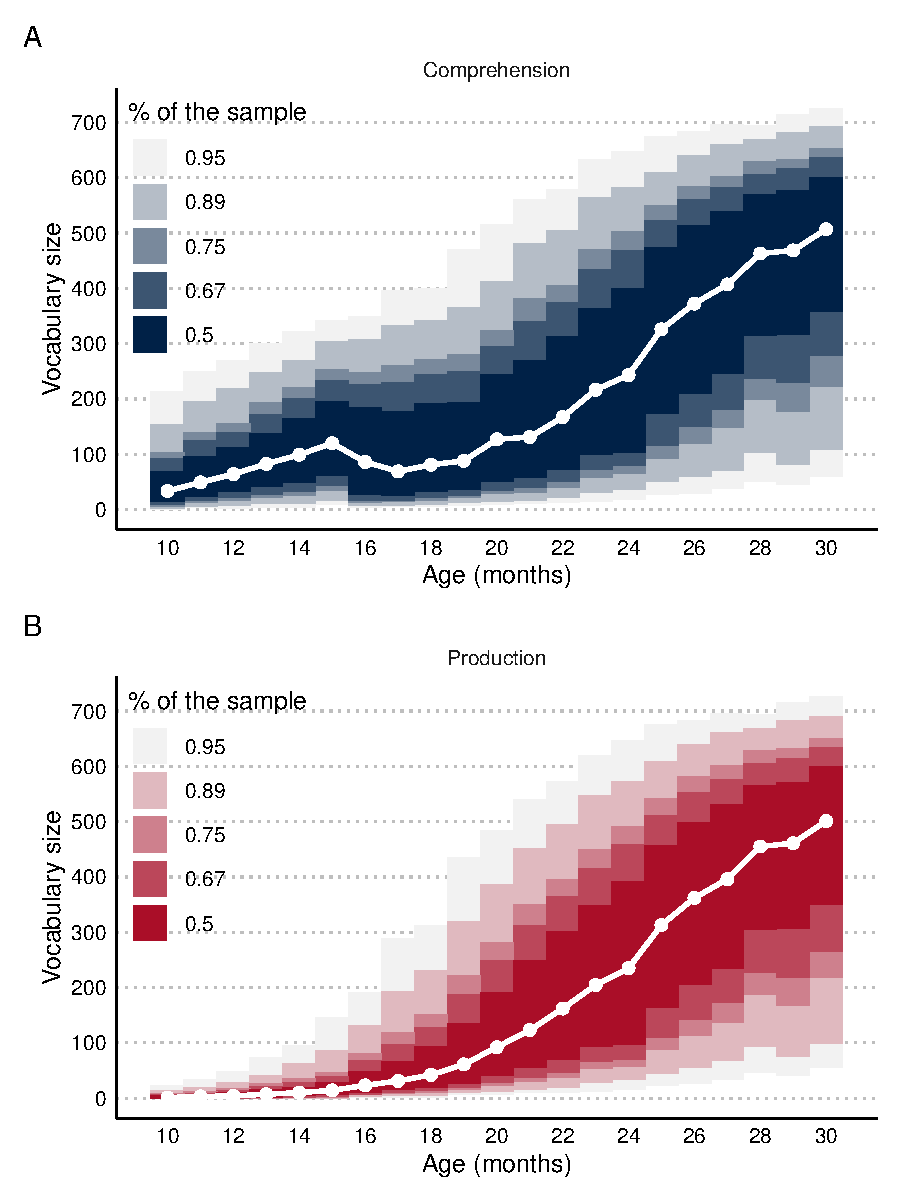
\includegraphics{chapters/01-introduction_files/figure-pdf/fig-wordbank-1.pdf}

}

\caption{\label{fig-wordbank}Wordbank norms for receptive (A) and
productive (B) vocabulary size in monolingual children. Vocabulary sizes
are expressed as the number of words that caregivers reported to be
acquired by their child, either as \emph{Understands} (receptive
vocabulary) or \emph{Undertands and Says} (productive vocabulary). Data
were collapsed for each month of age. Median vocabulary sizes for each
age group are indicated with white points and lines. Intervals of
different width (depicted with shades of colour) contain different
porportions of the sample.}

\end{figure}

\hypertarget{dynamics-of-early-lexical-access-and-selection}{%
\subsection{Dynamics of early lexical access and
selection}\label{dynamics-of-early-lexical-access-and-selection}}

There is some consensus in that the initial lexicon is only different
from the adult lexicon in quantitative terms. Many discontinuities and
non-linearities in the performance of infants and adults in word
recognition tasks can be explained as the result of differences in the
size of the lexicon. For instance, evidence of \emph{cascaded
activation} in the developing lexicon emerges at around 21 months,
associated to changes in the size of the lexicon. Cascaded accounts of
lexical processing describe how activation spreads across
representations at different levels in the lexicon, as the speech signal
unfolds, and is one of the most defining features of the adult lexicon
(Dell, 1986; Levelt, 1989). Most of these accounts assume, at least,
three levels of representation: conceptual, lexical, and phonological
(Caramazza, 1997). Lexical representations embody associations between
how words sound (\emph{phonological representations}, or word-forms) and
what words mean (\emph{semantic representations}, or concepts). During
word production and comprehension, representations from the three levels
are activated (lexical access), and one of them is selected for
comprehension or production (lexical selection). Which activations are
activated across the three levels is determined by bottom-up and
top-down sources of information. Figure~\ref{fig-lexicon-mon}
illustrates the dynamics in word comprehension.

\begin{figure}

{\centering 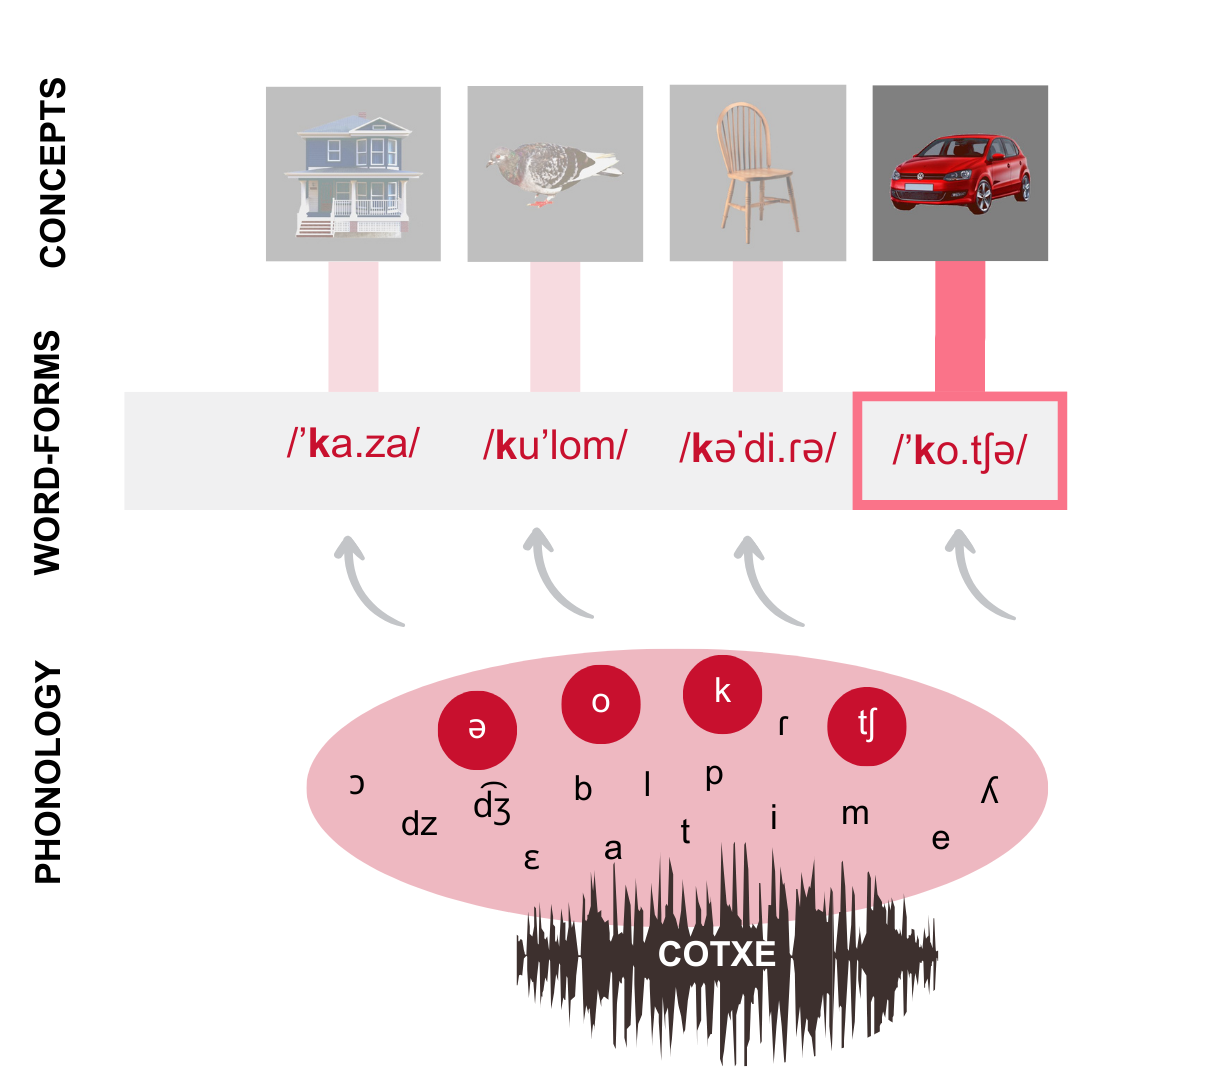
\includegraphics{chapters/../_assets/img/lexicon-mon.png}

}

\caption{\label{fig-lexicon-mon}Lexical access and selection in the
monolingual lexicon. The speech signal produced by a speaker uttering
the Catalan word \emph{COTXE} {[}car{]} activates phonological segments
in the listener's mental lexicon. Activation then spreads across lexical
representations containing such segments. In the illustration, a cohort
of words also starting with phoneme /k/ is activated. The phonological
form associated to the word \emph{COTXE} receives the strongest
activation, and is ultimately selected. In non-selected, but accessed,
lexical representations, activation spreads also to the semantic layer,
resulting in the activation of non-selected semantic representations.
Note that, for simplicity, we have used phonemes to depict phonological
units, but we acknowledge that phonological representations may be
encoded at the lower level of phonetic features.}

\end{figure}

Spoken word recognition starts with the acoustic-phonetic processing of
the speech signal. Phonological representations (e.g., articulatory
features, syllables, stress patterns) in the listener's mental lexicon
are activated according to how well they match the phonetic features and
co-articulatory information in the speech stream. Lexical
representations whose associated phonology matches the input are
activated. The set of lexical candidates then is modulated by multiple
factors: the degree of (mis)match with the unfolding acoustic input, the
dynamics of competition between lexical candidates (Luce \& Pisoni,
1998; McClelland \& Elman, 1986; Norris, 1994), and top-down information
like word frequency (Kukona et al., 2011), or grammatical,
suprasegmental, and semantic constraints provided by the sentential
context (Grosjean, 1980; W. Marslen-Wilson et al., 1988; Tyler \&
Wessels, 1983). Finally, the best-matching lexical representation is
selected, and its associated meaning is activated for comprehension.
This sequence of events occurs in a \emph{cascaded} fashion. Activation
spreads within and percolates across levels of representation while
lexical selection is still ongoing. Lexical representations sharing
phonological similarity (Grosjean, 1980; Luce et al., 1990; e.g., W. D.
Marslen-Wilson, 1987; W. D. Marslen-Wilson \& Welsh, 1978; McClelland \&
Elman, 1986) or semantic features (Collins \& Loftus, 1975; Mirman \&
Magnuson, 2009; Neely, 1977) are co-activated, and semantic
representations of activated lexical units are in turn retrieved, even
if their associated lexical representation is ultimately not selected.

A clear proof of cascaded activation at the phonological and semantic
levels was provided by Allopenna et al. (1998). The authors designed a
word-recognition task in which (adult) participants were presented with
four pictures on screen in each trial. Participants would then listen to
a command sentence like ``Pick up the \emph{casket}; now put it below
the diamond'', and perform the action. The authors manipulated the
phonological relationship between the target object's label (e.g.,
\emph{casket}), and the label of each of the three distractors. Two of
the distractors were phonologically related to the target, sharing onset
(e.g., \emph{castle}) or offset (e.g., \emph{basket}), respectively. The
other distractor was phonologically unrelated to the target (e.g.,
\emph{nickel}). After the onset of the auditory target label,
phonological distractors attracted participants' eye fixations more than
unrelated distractors. Distractors sharing phonological onset elicited
the effect at an earlier time window than those sharing phonological
offsets. Such time course of distractor fixations suggests that the
auditory presentation of the target label activated no only its
(subsequently selected) phonological representation in participants'
lexicon, but also that of phonologically related representations. In
summary, paradigms of spoken word recognition have proven useful in the
investigation of the structure of the adult lexicon: phonological and
semantic links between lexical representations are revealed as the
phonological or semantic relationship between the stimuli is
manipulated.

Priming paradigms of spoken word recognition have also provided strong
support for the existence of phonological and semantic links between
lexical representations before infants' second birthday. Arias-Trejo \&
Plunkett (2009) found that infants' spoken word recognition (e.g.,
\emph{dog}) was interfered by the previous presentation of a
semantically related word (e.g., \emph{cat}). This effect was found in
21-month-olds, but not in 18 month-olds. Styles \& Plunkett (2009)
reported semantic priming in 24-month-old participants but not in 18
month-old participants. Other studies have provided electrophysiological
evidence of semantic priming at earlier ages (Friedrich \& Friederici,
2005a; e.g., Rämä et al., 2013). Even in the absence of visual
referents, 24-month-old infants detect when strings of words presented
auditorily are semantically related, or when they are unrelated (Willits
et al., 2013). Overall, effects of semantic relations in word
recognition are observable in the initial lexicon.

Phonological priming effects also emerge around the same ages. Mani and
Plunkett (2010, 2011a) developed an implicit naming task in which each
trial started with the \emph{silent} presentation of a prime picture.
Then, a target-distractor picture pair was presented side-by-side.
Finally, the target picture's label was presented auditorily. The
authors manipulated the phonological overlap between the prime label and
the target label, so that in half of the trials both labels were
phonologically related, sharing phonological onset
(\emph{cat}-\emph{cup}), or phonologically unrelated
(\emph{ball}-\emph{comb}). Prime and target-distractor pairs were
semantically unrelated. At 18 and 21 months of age, English monolingual
infants showed different target looking preference patterns after
phonologically related prime pictures, compared to after phonologically
unrelated primes. This result suggests that infants implicitly named
prime pictures---despite such pictures were presented in silence---and
that the phonology of the resulting labels interacted with the
subsequent auditory target recognition. The direction of the effect was
different in both age groups. At 18 months, infants showed stronger
target preferences after being previously presented with a
phonologically related prime. But twenty-one month-olds' target
preference was weaker after phonologically related primes, compared to
after phonologically unrelated primes.

Mani \& Plunkett (2011a) interpreted this shift from facilitation to
inhibition as the consequence of the increase in vocabulary sizes of the
older infants. The authors suggested that, in sparser lexicons, the
fewer number of phonologically related lexical representations might
have led to faster selection of the target word. In larger lexicons,
lexical selection would be delayed by the cascaded activation of a
larger number of phonologically related lexical representations. In
support of this hypothesis, the authors found a positive significant
correlation between the size of the interference effect in 21 month-old
infants with two critical variables: participants' vocabulary size, and
the size of the phonological cohort of the presented words. Results by
Avila-Varela et al. (2021) provided converging evidence with German
monolinguals: larger interference effects were found in participants
with larger vocabulary sizes, even after controlling for age.

Chow, Aimola Davies, et al. (2017) provided further evidence of the
emergence of semantic \emph{and} phonological links, and it association
with lexical growth. The authors adapted the spoken word recognition
paradigm by Huettig \& McQueen (2007) to explore 24- to 30-month-old
toddlers. In each trial, participants were presented with four pictures.
Four seconds after, a word was auditorily presented. The authors
analysed participants visual fixations to each picture after the
auditory label was presented. In some trials, the auditory label
referred to one of the pictures. In other trials, it did not refer to
any of the pictures. In trials in which none of the pictures
corresponded to the presented label, one of the pictures was a
phonological distractor (its label shared phonological onset with the
presented label). Another picture was a semantic distractor (its
referent belonged to the same taxonomic category as the referent of the
presented word). For instance, participants were presented with the
pictures of a sandwich, a bus, a cat, and a dress. Then they would hear
the carrier phrase ``Look at the \emph{bee}!''. The picture of the bus
would be a phonological distractor (both words start with
/\textipa{b}/), and the cat would be a semantic distractor (bees and
cats are animals). Participants' visual fixations revealed a preference
for the phonological distractor at earlier stages of the post-naming
phase, and a preference for the semantic distractor at later stages of
the trial. These results are suggestive of a cascaded effect in spoken
word recognition in toddlers, in which the presentation of the auditory
word activated phonologically and semantically related lexical
representations. Visual preference for the distractors was stronger in
participants with larger vocabulary sizes, pointing to an association
between the strength of the connections across related lexical
representations and the growth of the lexicon.

In summary, previous studies on lexical access in monolingual toddlers
support a cascaded activation account of lexical access during the first
stages of lexical development, and point to a continuity between the
initial lexicon and the adult lexicon, bridged through vocabulary growth
during the second year of life.

\hypertarget{building-a-lexicon-in-two-languages}{%
\section{Building a lexicon in two
languages}\label{building-a-lexicon-in-two-languages}}

\hypertarget{defining-bilingualism}{%
\subsection{Defining bilingualism}\label{defining-bilingualism}}

One may consider \emph{bilingualism} a quite ill-defined term. In some
studies participants are classified as bilinguals with very low exposure
and command of a second language, while other studies require perfect,
native-monolingual proficiency of both languages for a participant to be
classified as bilingual. Since the present dissertation concerns
simultaneous bilingualism in infancy, we identify bilingualism with dual
language exposure. Quantitative language input is conventionally
operationalised as the cumulative amount of time the infant has spent
interacting with people who speak to them on a regular basis (e.g.,
parents, grandparents, siblings, daycare). In bilinguals, this
linguistic input is divided into two languages, which may be spoken by
the same of different people, at the same time or at different times.

Several instruments are available to measure language exposure in
bilinguals, usually involving a semi-structured interview with the
caregivers or detailed questionnaires that caregivers complete (e.g.,
Bosch \& Sebastian-Galles, 2001; Byers-Heinlein et al., 2020; Cattani et
al., 2014; DeAnda et al., 2016; Orena et al., 2020). The end-product is
generally a proportion of exposure to each of the languages, known as
\emph{Degree of Exposure} (DoE). The DoE reflects the cumulative amount
of input that the child has received in one language, relative to the
other. Although this measure is subject to biases and inaccuracies
induced by the subjective judgements of caregivers, there is evidence of
its external validity, as suggested by its high correlation with direct
measures of infant-directed speech (Orena et al., 2020). The underlying
assumption behind this measurement approach is that a child's linguistic
experience can be quantified into a continuous measure of bilingualism.
This score ranges from 0\% exposure to a second language (monolinguals)
to 50\% (perfectly balanced exposure to both languages). The language
exceeding 50\% DoE is referred to as the \emph{dominant} language of the
child, and the other language is referred to as the \emph{non-dominant}
language. For methodological simplicity, some studies classify
monolinguals and bilinguals into discrete categories. Although there is
not a strict threshold to consider a child as bilingual, most studies
consider a child as bilingual if they are exposed to a second language
at least 20\% of the time (Byers-Heinlein, 2015; Byers-Heinlein, Tsui,
Bergmann, Black, Brown, Carbajal, Durrant, et al., 2021; Rocha-Hidalgo
\& Barr, 2023a) (see Figure~\ref{fig-bilingualism} for a visual
illustration). This is the cut-off adopted in the present dissertation,
whenever such classification into discrete groups is methodologically
sound.

\begin{figure}

{\centering 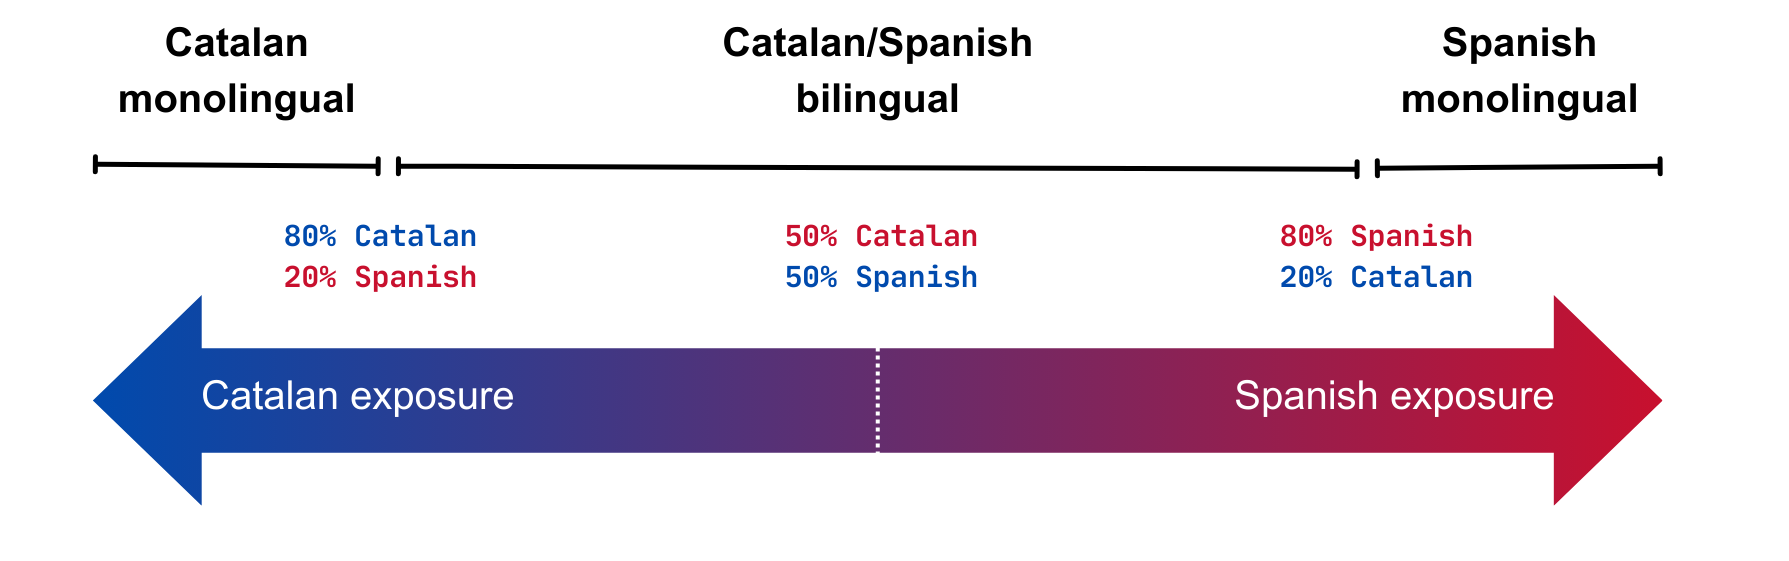
\includegraphics{chapters/../_assets/img/bilingualism.png}

}

\caption{\label{fig-bilingualism}Visual illustration of the
classification of participants dissertation into monolinguals and
bilinguals in the present dissertation. Participants' relative exposure
to Catalan and Spanish ranged from completely Catalan (in blue) to
completely Spanish (in red). In agreement with the consensus in the
firld, we classified participants into monolinguals and bilinguals by
setting a threshold of 20\% degree exposure to the language of least
exposure. Participants with a relative exposure to a second language
higher than 20\% were classified as bilinguals, and as monolinguals
otherwise.}

\end{figure}

\hypertarget{bilingual-word-acquisition}{%
\subsection{Bilingual word
acquisition}\label{bilingual-word-acquisition}}

Bilinguals acquire language in a more challenging set of circumstances
than monolinguals. First, there is little reason to think that
bilinguals receive a larger amount of language exposure than their
monolingual peers. Given that bilinguals' linguistic input is divided
into two languages, they receive less exposure in each of their
languages than monolinguals do. Second, bilinguals need to learn two
codes, which might overlap to different degrees: two phonologies, two
grammatical systems, and two lexicons. Third, the referential context in
which bilinguals build a lexicon is also more complex. Bilinguals
frequently learn at least two labels for the same referent, one for each
language. The concepts behind both labels may not align perfectly. For
instance, a child learning English and Spanish might learn the words
\emph{finger} and \emph{dedo} (its Spanish translation). While both
words might be used to refer to the same referent (e.g., the index
\emph{finger}), the word finger refers to eight appendices (four in each
hand), whereas \emph{dedos} refers to 20 appendices (five in each hand
and five in each foot). In summary, bilinguals are presented with a more
complex linguistic environment, facing additional demands compared to
their monolingual counterparts.

Such increased cognitive demands do not keep bilinguals from reaching
major language acquisition milestones at similar ages as monolinguals
(see Sebastian-Galles \& Santolin, 2020a for review), as observed in
language discrimination (Bosch \& Sebastian-Galles, 2001; Bosch \&
Sebastián-Gallés, 1997; Byers-Heinlein et al., 2010; Nacar Garcia et
al., 2018; Sebastián-Gallés et al., 2012; Weikum et al., 2007),
discrimination of native phonemic contrasts (Albareda-Castellot et al.,
2011; Bosch \& Sebastián-Gallés, 2003; Burns et al., 2007; Sundara et
al., 2006, 2008), or word-form segmentation (Antovich \& Graf Estes,
2018; Bosch et al., 2013; Houston \& Jusczyk, 2000; Hurtado et al.,
2014; Nazzi et al., 2006; Polka et al., 2002; A. S. M. Tsui et al.,
2021). During the second year of age, bilinguals also undergo the same
increase in vocabulary size that monolinguals go through (Core et al.,
2013; Hoff et al., 2012; e.g., Pearson \& Fernández, 1994). As in
monolinguals, spoken word recognition becomes more efficient as the
infant's lexicon expands (De Anda \& Friend, 2020; DeAnda et al., 2018;
Legacy et al., 2018; Poulin-Dubois et al., 2013a, 2017). Such changes
are modulated by the relative amount of input that the bilingual infant
receives from each language. For instance, bilinguals acquire words
faster, and become more efficient at spoken word recognition in their
dominant language, compared to the non-dominant language (Cattani et
al., 2014; Floccia, Sambrook, Delle Luche, Kwok, Goslin, White, Cattani,
Sullivan, Abbot‐Smith, et al., 2018; Hoff, 2003; Marchman et al., 2010;
Shneidman et al., 2013; Thordardottir, 2011). Overall, the monolingual
and the bilingual lexicons grow at a similar rate, but some studies
suggest that bilingualism may modulate word learning trajectories.

Hoff et al. (2012) collected vocabulary size data from a cohort of 103
infants at two age points at 22 and 30 months. Infants were being raised
in English monolingual or English-Spanish bilingual homes in South
Florida (United States). Both groups had equivalent socio-demographic
backgrounds. Families of English monolingual infants filled in the MCDI,
and families of English-Spanish bilinguals filled the MCDI and its
Spanish adaptation, the \emph{Inventario del Desarrollo de Habilidades
Communicativas} (Jackson-Maldonado et al., 1993). Monolinguals showed
the largest English vocabulary sizes, followed by English-dominant
bilinguals, and Spanish-dominant bilinguals. The reverse pattern was
observed for Spanish vocabulary sizes. When Hoff et al. (2012) combined
the vocabulary English and Spanish vocabulary sizes into a single
measure of \emph{total} vocabulary, monolinguals and bilinguals showed
equivalent vocabulary sizes. These results indicate that bilinguals keep
up with monolinguals in vocabulary growth (Bosch \& Ramon-Casas, 2014;
Byers-Heinlein et al., 2023a; Core et al., 2013; see also Pearson et
al., 1993; Pearson \& Fernández, 1994; Poulin-Dubois et al., 2013a), and
highlight the importance of comparing monolingual and bilingual
trajectories of lexical acquisition sizes taking both languages into
account (Bedore et al., 2005).

Not all bilingual populations have shown equivalent patterns of lexical
development. For instance, studies in other populations of bilinguals
have reported differences in total vocabulary size in monolinguals and
bilinguals, and equivalent conceptual vocabulary sizes. This suggests
that bilinguals may acquire a larger number of words across both
languages than monolinguals, corresponding to an equivalent number of
lexicalised concepts in both groups (De Houwer et al., 2014; Siow et
al., 2023), or even higher (Kern et al., 2019). These results suggest
that the specific pair of languages that bilinguals learn must be taken
into consideration when investigating the early stages of lexical
development. Participants in Hoff et al. (2012) were learning English
and Spanish. These two languages are relatively distant in typological
terms. English is a Germanic language, while Spanish is a Romance
language. In addition to their differences in grammar or phonology,
English and Spanish also share fewer cognates than other pairs of
languages like Italian and Spanish (Schepens et al., 2012). Recent
studies have reported that bilingual learning two languages that share a
higher amount of cognates may acquire words at a faster rate than those
learning two languages sharing fewer cognates (Floccia, Sambrook, Delle
Luche, Kwok, Goslin, White, Cattani, Sullivan, Abbot‐Smith, et al.,
2018; Gampe et al., 2021). This might explain some of the variability
observed in the characterisation of lexical growth across different
bilingual populations.

\hypertarget{language-non-selectivity-in-the-bilingual-lexicon}{%
\section{Language non-selectivity in the bilingual
lexicon}\label{language-non-selectivity-in-the-bilingual-lexicon}}

Floccia, Sambrook, Delle Luche, Kwok, Goslin, White, Cattani, Sullivan,
Abbot‐Smith, et al. (2018) conducted an impressive study of CDI
responses were collected from a large sample of 372 bilinguals at
24-months of age. These bilinguals were learning English and an
additional language---one of Bengali, Cantonese, Dutch, French, German,
Greek, Hindi-Urdu, Italian, Mandarin, Polish, Portuguese, Spanish, and
Welsh. Participants were raised in the United Kingdom, and English was
the dominant language for most of them. Using an edit distance-based
metric of similarity, the authors calculated the phonological similarity
between the translation equivalents present in the English vocabulary
checklist, and in the vocabulary checklist of each of the other
languages. The average phonological similarity between English and each
pair of languages was taken as a proxy to their lexical similarity. Some
language pairs shared high lexical similarity (e.g., English-Dutch),
while others shared very little (e.g., English-Mandarin). The authors
then estimated the association between lexical similarity and
participants' language outcomes---measured as their receptive and
productive vocabulary size in English and the additional
language---while adjusting for the influence of other predictors like
age, sex, socio-economic status, and several properties of participants'
speech input. Bilinguals' vocabulary size in the additional language
showed a lexical similarity effect, in which children learning two
lexically similar languages showed larger vocabulary sizes in the
additional language, while English vocabulary did not show such
association with lexical similarity. Overall, the results suggest that
infants may benefit from the lexical similarity between their
languages--particularly, by the presence of cognates---and therefore
bilinguals' trajectories of word acquisition should be considered in the
context of the pair of languages being learned.

A facilitation effect at the lexical level would have important
consequences for infants learning highly similar languages. For intance,
the relative typological distance between Catalan and Spanish is very
small, especially at the lexical level. Both are Romance language, and
share many cognates (i.e., form-similar translation equivalents).
Figure~\ref{fig-cat-spa-distance} shows the overall lexical similarity
between Catalan and Spanish, computed in the same way that Floccia,
Sambrook, Delle Luche, Kwok, Goslin, White, Cattani, Sullivan,
Abbot‐Smith, et al. (2018) did. The lexical similarity between Catalan
and Spanish is considerably larger than that of English and Dutch, the
language pair with the highest similarity score in Floccia et al.~This
suggests that Catalan-Spanish bilinguals might be exposed to a
substantially larger amount of cognates than bilinguals learning English
and and additional language, like those in Floccia, Sambrook, Delle
Luche, Kwok, Goslin, White, Cattani, Sullivan, Abbot‐Smith, et al.
(2018) and Hoff et al. (2012). If linguistic similarity, and especially
lexical similarity, play a facilitative role in bilingual word
acquisition, Catalan-Spanish bilinguals should show an even larger
effect. This might explain why bilinguals in our database display larger
vocabulary sizes than monolinguals, in contrast with the equivalent
total vocabulary sizes reported by Hoff et al. (2012) in English-Spanish
bilinguals (learning two languages sharing less lexical similarity).

\begin{figure}

{\centering 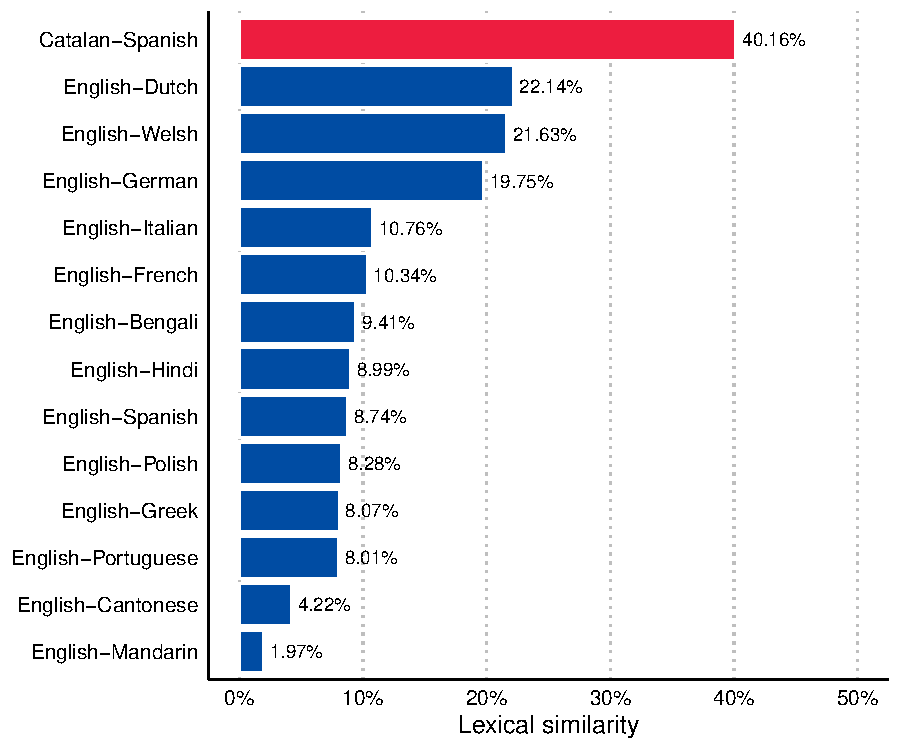
\includegraphics{chapters/01-introduction_files/figure-pdf/fig-cat-spa-distance-1.pdf}

}

\caption{\label{fig-cat-spa-distance}Lexical similarity between Catalan
and Spanish, and between English and each of the additional languages in
Floccia et al.~(2018). We first obtained the broad phonological
transcriptions of the words included in the Catalan and Spanish
vocabulary checklists of the BVQ. Catalan words were transcribed to the
Central Catalan variant (the most prevalent in the Metropolitan Area of
Barcelona), and Spanish words were transcribed to Castilian Spanish.
Interjections and onomatopoeic words were excluded. We then computed the
normalised Levenshtein between each pair of translation equivalents, and
averaged them.}

\end{figure}

The facilitation effect of lexical similarity on vocabulary growth
reported by Floccia, Sambrook, Delle Luche, Kwok, Goslin, White,
Cattani, Sullivan, Abbot‐Smith, et al. (2018) points to a possible
cognateness facilitation effect on word acquisition, in which cognates
are acquired at earlier ages than non-cognates. In this scenario,
bilinguals learning languages that share more cognates would acquire
words faster than those learning two languages that share fewer
cognates. In line with this claim, previous studies had provided
evidence in favour of an earlier age of acquisition for cognates. For
instance, some studies have reported a larger proportion of cognates in
bilinguals' lexicons than the proportion of non-cognates (Bosch \&
Ramon-Casas, 2014; Fabian, 2016; Schelletter, 2002). Other studies have
found that bilinguals' performance in word recognition tasks is
increased for cognate words, relative to non-cognate words (Gampe et
al., 2018). More recent evidence in English-French bilingual suggest
that cognates are may be more likely to be acquired than non-cognates at
early ages (Mitchell et al., 2022). The specific mechanisms behind an
earlier age of acquisition for cognates, however, are unclear.

To explain the facilitation effect of lexical similarity on vocabulary
growth, Floccia, Sambrook, Delle Luche, Kwok, Goslin, White, Cattani,
Sullivan, Abbot‐Smith, et al. (2018) suggested that the \emph{parallel
activation} of cognates during language exposure might boost their
acquisition. The notion of \emph{parallel activation} stems from the
language non-selective hypothesis of bilingual lexical processing. This
hypothesis states that bilinguals co-activate lexical representations
from both languages during language production and comprehension, even
in monolingual situations. This parallel co-activation is the result of
cascaded activation spreading across the two languages at multiple
levels of word recognition and production. This hypothesis was initially
proposed to account for different results in adult bilingual research.

Marian \& Spivey (1999) presented Russian-English adult bilinguals with
an cross-language interference task, divided in two blocks. In one
block, participants would be presented with an instruction in English,
like ``Put the \emph{marker} below the cross'', after which two pictures
were displayed on the screen. One depicted the target object (a stamp).
The other depicted an object whose label in Russian shared phonetic
features with the English target label (e.g., a stamp, \emph{marka} in
Russian). In the other block, the same procedure would be followed, but
now with Russian as the target language. Participants were presented
with the Russian instruction: ``\emph{Poloji} glaz \emph{nije
krestika}'' {[}Put the \emph{eye} below the cross{]}. The target picture
would be an eye, and the distractor, a glove, whose English label shared
phonetic features with the Russian target label. In both blocks, a
control condition was run, in which target and distractor labels were
phonetically unrelated. In line with Allopenna et al. (1998)'s results
in monolingual adults, after hearing the target label, bilinguals
fixated the cross-language phonological distractor significantly more
than the unrelated distractors. These findings suggest that participants
activated phonologically related word-forms in both Russian \emph{and}
English, which affected their overt visual exploration patterns during
the task. In this case, parallel activation is driven by bottom-up
activation of words in both languages through phonology, at a
sub-lexical level. Words that sound the same in both languages are
activated, and enter the cohort during lexical selection.
Figure~\ref{fig-lexicon} illustrates this sequence of events.

\begin{figure}

{\centering 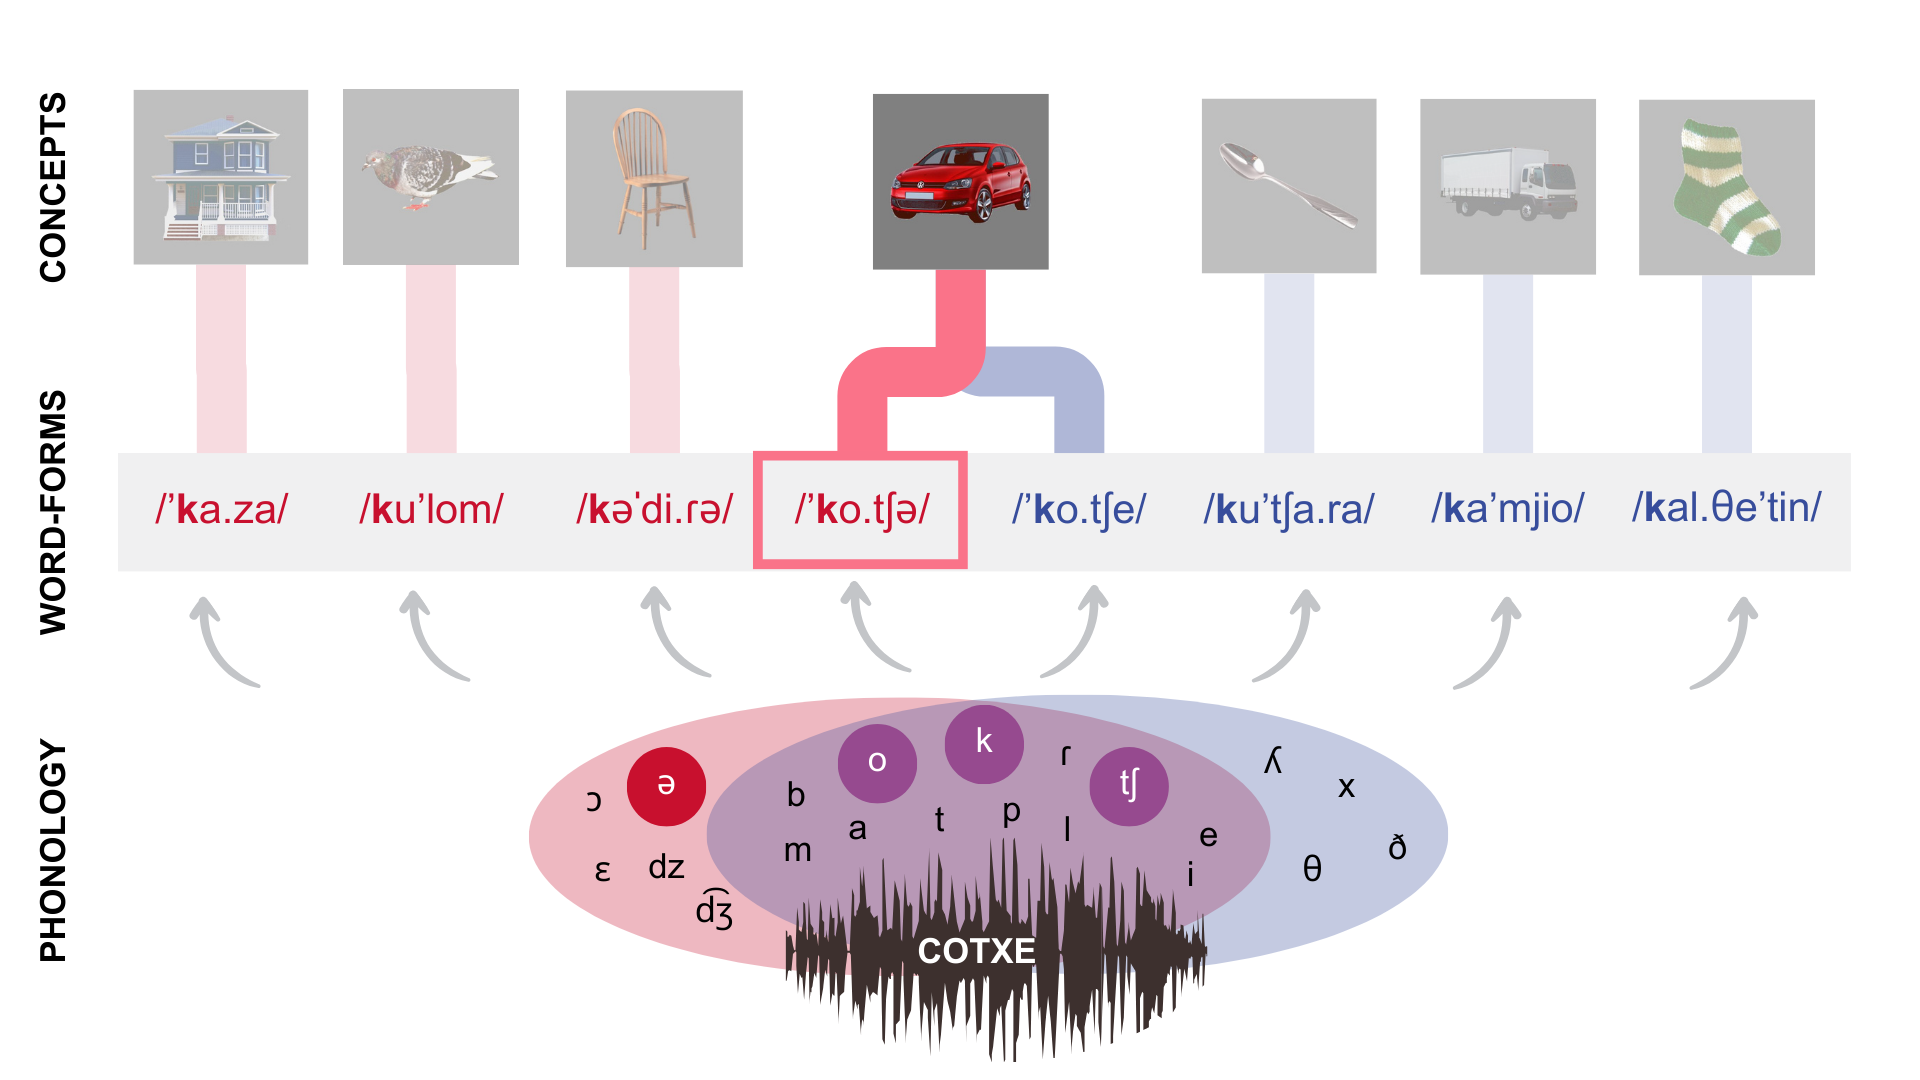
\includegraphics{chapters/../_assets/img/lexicon.png}

}

\caption{\label{fig-lexicon}Lexical access and selection in the
language-non selective bilingual lexicon. The speech signal produced by
a speaker uttering the Catalan word \emph{cotxe} {[}car{]} activates
phonological segments in the repertoire of a Catalan-Spanish bilingual
listener. Activation spreads across lexical representations in both
languages that contains such segments. In the illustration, a cohort of
words that also start with the /k/ phoneme are activated. The word-form
associated to \emph{cotxe} receives the strongest activation, and is
ultimately selected. In non-selected, but accessed, lexical
representations, activation percolates to the semantic layer, resulting
in the activation of non-selected semantic representations.}

\end{figure}

Parallel activation can also be the result of cascaded activation
spreading across lexical representations in both languages, through
their shared semantic features. Previous studies have provided strong
evidence of parallel activation in exclusively monolingual tasks by
comparing the processing of cognates and non-cognates. In Costa et al.
(2000), adult Catalan-Spanish bilinguals and Spanish monolinguals were
asked to name pictures of common objects in Spanish. In half of the
trials, the object labels were cognates in Catalan and Spanish
(\emph{sofà}-\emph{sofá}, translations of \emph{sofa}). In the other
half of the trials labels were non-cognates (\emph{taula}-\emph{mesa},
translations of \emph{table}). Bilinguals named cognate pictures faster
than non-cognate pictures, even after adjusting for the lexical
frequency of the items. Spanish monolinguals showed equivalent naming
times for the two categories, as the distinction was meaningless to
them. These results suggested that, in bilinguals, the Catalan
phonnology was activated, facilitating Spanish word production: the
visual recognition of the pictures led to the activation of their
corresponding semantic representations, resulting in the cascaded
activation of phonological representations in both languages.

In adults, the available evidence in favour of language non-selectivity
in the bilingual lexicon is abundant across languages (Bobb et al.,
2020; Colomé, 2001; Costa et al., 1999, 2000; Duñabeitia et al., 2009;
Duyck, 2005; Hoshino \& Kroll, 2008; Marian \& Spivey, 2003; Spivey \&
Marian, 1999; Thierry \& Wu, 2007), including sign languages (Giezen \&
Emmorey, 2016; Gimeno-Martínez et al., 2021a; Van Heuven et al., 1998).
Modelling efforts have successfully implemented formal accounts of the
bilingual lexicon by incorporating cross-language interactions (Dijkstra
et al., 2019; Dijkstra \& Van Heuven, 2002; e.g., Kroll et al., 2010;
Kroll \& Stewart, 1994). In summary, there is consensus about the fact
that bilinguals constantly co-activate both languages during word
comprehension and production, even in fully monolingual situations.

Previous studies have provided evidence in of language non-selectivity
in the initial bilingual lexicon (Bosma \& Nota, 2020; Jardak \&
Byers-Heinlein, 2019; Poarch \& Van Hell, 2012; Poulin-Dubois et al.,
2013a, 2017; Singh, 2014; Von Holzen et al., 2019a; Von Holzen \& Mani,
2012a). Priming paradigms of word recognition tasks have been
instrumental in this line of research. Using one of such paradigms, Von
Holzen \& Mani (2012a) reported evidence of cross-language phonological
priming in 21- to 42-months-old children learning German and English. At
the beginning of each trial, the authors presented an auditory prime
word in English. Then, the auditory target label was presented in
German. Finally the target and distractor pictures were presented
side-by-side. Participants' looking preference towards the target was
recorded, and interpreted as a proxy of target word recognition. The
authors manipulated the phonological overlap between the prime and
target labels. In some trials, the English prime label and the German
target label labels were phonologically related through translation: the
prime label did \emph{not} overlap with the target label in English
(e.g., \emph{leg}-\emph{Stein} {[}\emph{stone}{]}), but its translation
in German did {[}\emph{Bein}{]}. In the rest of the trials prime and
target labels were phonologically unrelated in both languages. The
authors found a stronger target picture looking preference in unrelated
trials, compared to trials in the priming-through-translation condition.
This suggests that participants activated the German translation of the
auditory English prime word, and that this interfered with the
recognition of the auditory German target word (which shared
phonological similarity with the German translation).

Priming studies in which words from both languages are presented during
the same experimental session or even within the same trial (Floccia et
al., 2020; Jardak \& Byers-Heinlein, 2019; Singh, 2014; e.g., Von Holzen
\& Mani, 2012a) present an important methodological pitfall. In these
tasks, participants are introduced in a bilingual context, in which the
overall degree of activation of lexical representations in both
languages may be artificially increased (Grosjean, 1997). This might
have contributed, to some extent, to the strength of the parallel
activation reported in these studies. It is possible that, in the daily
life of a sizeable amount of bilingual children, speech input in each
language takes place at separate times and unlikely that they take place
within the same communicative act. If this is the case, the practical
relevance of language non-selectivity in vocabulary growth might be
smaller than anticipated.

In summary, the parallel activation hypothesis suggested by Floccia,
Sambrook, Delle Luche, Kwok, Goslin, White, Cattani, Sullivan,
Abbot‐Smith, et al. (2018) to explain the cognateness facilitation
effect relies on the language non-selectivity of the early lexicon. But
experimental evidence in the developing lexicon for such language
non-selectivity builds on experimental paradigms that may overestimate
the amount of co-activation between the two languages, as they put
participants in a bilingual context that might forcibly lead to both
languages being active.

\hypertarget{the-present-dissertation}{%
\section{The present dissertation}\label{the-present-dissertation}}

The aim of this dissertation is to explore the impact of language
non-selectivity on the developing bilingual lexicon, and its potential
role in the facilitation effect of lexical similarity during vocabulary
growth. In Chapter 2, we put forward an account of bilingual word
acquisition, inspired in accumulator models of word language acquisition
(Hidaka, 2013; Kachergis et al., 2022a; McMurray, 2007; Mollica \&
Piantadosi, 2017a). This model provides a mechanistic explanation for
the facilitative effect of lexical similarity reported by Floccia,
Sambrook, Delle Luche, Kwok, Goslin, White, Cattani, Sullivan,
Abbot‐Smith, et al. (2018). It describes an interplay between the
lexical frequency of a word, the child's relative exposure to each
language, and cross-language phonological similarity. In this model,
bilinguals accumulate experience with words in one language, even when
listening to words in the other language. We contrast this model against
vocabulary data from bilinguals, collected using an \emph{ad hoc} online
questionnaire. This questionnaire was inspired in the CDI, adapted to
the population of bilinguals learning Catalan and Spanish in the
Metropolitan Area of Barcelona (Spain). We modelled the acquisition
trajectories of 302 translation equivalents, testing the role of
cognateness and its interaction with relative language exposure and
lexical frequency with.

The predictions tested in Chapter 2 rely on the assumption that
bilingual infants co-activate translation equivalents in both languages,
even in monolingual situations. Although there is evidence in favour of
cross-language activation in toddlers, as just said, previous studies
have relied on experimental paradigms in which participants listen to
words from both languages in each trials. This puts participants in a
bilingual context in which parallel activation might result from an
overall stronger activation of both languages induced by the
experimental task, and not because of regular cascaded activation across
languages. In Chapter 3, adapting the implicit naming paradigm by Mani
and Plunkett (2010, 2011a) we test parallel activation in an exclusively
monolingual task. As described in the Methods section of Chapter 2, this
paradigm is a word recognition task in which priming stimuli are
pictures presented in silence. Previous studies shown that infants at 18
months and older lexicalise pictures presented in silence (Duta et al.,
2012; Mani \& Plunkett, 2010, 2011a; Styles et al., 2015). In
particular, Mani and Plunkett (2010, 2011a) found that word recognition
is influenced by the prior presentation of a picture whose associated
label is phonologically related to the target word. By manipulating the
cognate status of the label associated to the prime image, we tested
parallel activation in bilingual toddlers while avoiding the
presentation of words in both languages.

The final chapter of this dissertation provides a summary of the
findings of Chapters 2 and 3. We discuss their implications for the
current understanding of the initial lexicon, and of how bilingualism
shapes infants' trajectories of word acquisition.

\bookmarksetup{startatroot}

\hypertarget{chapter-2-cognate-beginnings-to-bilingual-lexical-acquisition}{%
\chapter{Chapter 2: Cognate beginnings to bilingual lexical
acquisition}\label{chapter-2-cognate-beginnings-to-bilingual-lexical-acquisition}}

\begin{tcolorbox}[enhanced jigsaw, opacitybacktitle=0.6, bottomrule=.15mm, arc=.35mm, title=\textcolor{quarto-callout-note-color}{\faInfo}\hspace{0.5em}{Note}, toprule=.15mm, bottomtitle=1mm, rightrule=.15mm, colbacktitle=quarto-callout-note-color!10!white, toptitle=1mm, opacityback=0, leftrule=.75mm, coltitle=black, left=2mm, colframe=quarto-callout-note-color-frame, titlerule=0mm, colback=white, breakable]

This Chapter has been preivously pusblished as a pre-print at PsyArxiv:

Garcia-Castro, G., Avila-Varela, D., Castillejo, I., \&
Sebastian-Galles, N. (2023). Cognate beginnings to bilingual lexical
acquisition. \url{https://doi.org/10.31234/osf.io/dxsmz}

\end{tcolorbox}

\hypertarget{introduction-1}{%
\section{Introduction}\label{introduction-1}}

The foundations of word learning are in place at an early age. At six
months, infants start directing their gaze to objects when hearing their
labels (Bergelson \& Swingley, 2012b, 2015; Tincoff \& Jusczyk, 1999b),
and shortly after caregivers start reporting some words as acquired by
their infant in vocabulary checklists (e.g., Fenson et al., 2007;
Samuelson, 2021). Most research on early word acquisition relies
extensively on data from monolingual children, and is oblivious to the
fact that a substantial proportion of the world population acquires more
than one language from early ages (Grosjean, 2021). Previous work on
bilingual vocabulary acquisition pointed to bilingual toddlers knowing,
on average, less words in each of their languages than their
monolinguals peers, and to both groups knowing a similar number of
words---if not more words---when the bilinguals' two languages are
pooled together. Hoff et al. (2012) found that English-Spanish bilingual
toddlers in South Florida (United States) knew less words in English
than monolinguals did, but both groups knew a similar total amount of
words when both English and Spanish vocabularies were counted together.
Other studies have provided converging evidence that bilinguals know a
similar or even larger number of words than monolinguals when the two
languages are aggregated (Gonzalez-Barrero et al., 2020; Oller \&
Eilers, 2002; Patterson, 2004; Patterson \& Pearson, 2004; Pearson \&
Fernández, 1994; Smithson et al., 2014). A more detailed analysis of the
words in bilinguals' lexicons shows some interesting patterns.

One important observation of studies on bilinguals' early vocabulary
acquisition is that cognate words are easier to acquire than non-cognate
words. Cognate words are translation equivalents that are phonologically
similar (or share some type of form-similarity). For instance, the
Spanish translation equivalent of cat is \emph{gato}, a cognate word;
the translation equivalent of dog is \emph{perro}, a non-cognate word.
For historical reasons, some pairs of languages share more cognates than
others: languages typologically close (like Dutch and English or Italian
and Spanish) share more cognates than languages typologically distant
(like English and Chinese, or Urdu and Spanish). The conclusion that
cognate words are easier to learn is based on two types of evidence:
studies investigating vocabulary sizes in children learning language
pairs with different percentages of cognates (that is, differing in
their typological distance) and studies comparing the number of cognate
and non-cognate words children know in a specific language pair.

Floccia, Sambrook, Delle Luche, Kwok, Goslin, White, Cattani, Sullivan,
Abbot‐Smith, et al. (2018) published an impressive study comparing
vocabularies of children learning several language pairs differing in
their percentage of cognates. The authors collected vocabulary data on
word comprehension and production from 372 24-month-old bilingual
toddlers living in the United Kingdom who were learning English and an
additional language. The additional language was one of 13 typologically
diverse languages: Bengali, Cantonese Chinese, Dutch, French, German,
Greek, Hindi or Urdu, Italian, Mandarin Chinese, Polish, Portuguese,
Spanish, and Welsh. The authors calculated the average lexical overlap
between the words in each of these additional languages and their
translation equivalents in English. Lexical overlap was calculated in
terms of phonological similarity (described below) and it was taken as a
proxy of the degree of cognateness between each pair of languages.
Floccia and co-workers reported an increase in vocabulary size in the
additional language (i.e., not English) associated with an increase in
the average phonological similarity between the translation equivalents
of each language pair. For example, English-Dutch bilinguals (languages
with a high phonological overlap), were able to produce more Dutch words
than English-Mandarin bilinguals (languages with a low phonological
overlap) were able to produce in Mandarin. Blom et al. (2020b), Bosma et
al. (2019), and Gampe et al. (2021) reported similar results, providing
converging evidence of a facilitatory effect of a lower language
distance (i.e., higher degree of cognateness) on vocabulary size.

A second set of studies suggested that cognates are overrepresented in
bilinguals' early lexicon. Bosch \& Ramon-Casas (2014) collected
parental reports of expressive vocabulary from 48 Catalan-Spanish
bilinguals aged 18 months and found that cognates represented a larger
proportion of vocabulary than non-cognates. Schelletter (2002) provided
converging evidence from a longitudinal single-case study, in which an
English-German bilingual child produced cognates earlier than
non-cognates, on average. But the high proportion of cognates in the
vocabulary of the participants in these two studies may not necessarily
evidence of a facilitation effect of cognateness, but rather of simply
the high proportion of cognates present in the pair of languages being
learned. For instance, if two given languages share a high proportion of
cognates like 70\%, the vocabulary contents of children learning both
languages should, in principle, approximate such proportion of cognates,
even in the absence of a cognateness facilitation effect. More recently,
Mitchell et al. (2022) addressed this issue in a longitudinal study. The
authors collected expressive vocabulary data of 47 16- to 30-month-old
French-English bilinguals living in Canada, in both languages. They
created two lists of translation equivalents; one made of 131 cognates,
and one made of 406 non-cognates. Across ages, the proportion of words
that children were reportedly able to produce was higher in the cognate
lists than in the non-cognate list. Critically, this difference
persisted after both lists were matched in size, controlling their
semantic category (i.e., furniture, animals, food were similarity
represented in both lists) and age-of-acquisition norms (an index of
word difficulty). Taken together, the results of these two lines of
research support the hypothesis that phonological similarity (as
reflected in cognateness) plays a facilitation role in bilingual word
learning.

Parallel activation of bilinguals' lexicons has been proposed as the
underlying mechanism for such facilitatory effect (e.g., Floccia,
Sambrook, Delle Luche, Kwok, Goslin, White, Cattani, Sullivan,
Abbot‐Smith, et al., 2018; Mitchell et al., 2022). The parallel
activation hypothesis stems from the language non-selective account of
lexical access, which suggests that bilinguals activate both languages
simultaneously during language processing, even in fully monolingual
contexts. Evidence with adult bilinguals supporting the language-non
selective account of lexical access has been reported for language
comprehension and production, across the auditory and visual (reading
and signing) modalities (Gimeno-Martínez et al., 2021b; Hoshino \&
Kroll, 2008; Morford et al., 2011; Shook \& Marian, 2012; Spivey \&
Marian, 1999; see Kroll \& Ma, 2017 for review). One of the clearest
pieces of evidence of parallel activation was provided by Costa et al.
(2000). In this study, Spanish monolinguals and Catalan-Spanish
bilingual adults were asked to name pictures of common objects in
Spanish. In half of the trials, the object labels were cognates in
Spanish and Catalan (árbol-arbre, translations of tree), whereas in the
other half of the trial labels were non-cognates (mesa-taula,
translations of table). Obviously, such distinction was only relevant
for bilinguals. Bilinguals named cognate pictures faster than
non-cognate pictures, even after adjusting for the lexical frequency of
the items. In contrast, Spanish monolinguals, who were unfamiliar with
the Catalan translations of the Spanish words they uttered, showed
equivalent naming times for the two types of stimuli. The authors
interpreted the difference between cognates and non-cognates in
bilinguals as reflecting the additional phonological activation that
cognate words would receive from their translation equivalents (due to
language non-selective activation of bilinguals' lexicons). These
results showed that bilinguals' Catalan phonology was activated during
the production of Spanish words, facilitating the naming of cognate
pictures. More recently, evidence of parallel activation has been
reported in bilingual toddlers and children too (Bosma \& Nota, 2020;
Floccia et al., 2020; Poarch \& Hell, 2012; Poulin-Dubois et al., 2013b;
Von Holzen et al., 2019b; Von Holzen \& Mani, 2012b). Although there is
a consensus on the role of parallel activation in bilinguals' lexical
processing and acquisition, previous studies do not address its
influence on the learning trajectories of individual words. Results are
aggregated across words and provide no information about the specific
dynamics of how parallel activation influences word learning. This is
the goal of the present research.

We propose an account in which a learning instance for a word may also
represent a learning instance for its translation equivalent, to the
extent that such translation equivalent is co-activated. We use the term
learning instance in the fashion of accumulator models of language
acquisition; as an exposure to a word-form that constitutes an
opportunity for the child to accumulate information about the word. We
do not assume if a learning instance is a discrete or a continuous unit
of accumulation of information. We consider that a learning instance of
a word is an exposure to its (phonological) form if the resulting
strength of activation of its representation in the child's lexicon
reaches some thoretical threshold that leads to word-form recognition.
This activation may result from the infant being exposed to the actual
word-form, or the result of activation spreading through phonological or
semantic links across lexical representation, as in the case of parallel
activation. The strength of this co-activation is proportional to the
phonological similarity between the two translation equivalents; given
that cognates share higher phonological similarity than non-cognates,
the former should be co-activated more strongly than the latter. This
should lead to a faster accumulation of learning instances for cognates,
compared to non-cognates. Parallel activation would allow bilingual
children to accumulate learning instances for words in both languages
even during fully monolingual situations, but the impact of this
mechanism would be asymmetric across languages: words from the
lower-exposure language would receive stronger activation from words in
the higher-exposure language than vice versa. Therefore, the acquisition
of words from the lower-exposure language would benefit more strongly
from their cognate status than the acquisition of words from the
higher-exposure language. This asymmetric cross-language activation
would be consistent with previous reports of larger priming effects from
the dominant to the non-dominant language (e.g., Grainger, 1998).

Consider the example of the Catalan-Spanish cognate translation
equivalent /\textipa{"gat}/--/\textipa{"ga.to}/ {[}cat{]}, which are
phonologically very similar. When the child listens to /\textipa{"gat}/,
they will strongly co-activate /\textipa{"ga.to}/ in parallel. If the
child has already formed a form-meaning association for both word-forms,
parallel activation may result from the activation of their common
concept or from activation spreading through phonological similarity. We
assume semantic co-activation to be constant across cognate and
non-cognate translation equivalents, and focus on phonological
co-activation as an additional source of activation that affects
cognates more strongly than non-cognates. Therefore, this exposure will
count as a learning instance for both co-activated forms. The case of
the non-cognate translation equivalent
/\textipa{"gos}/--/\textipa{"pe.ro}/ {[}dog{]} would be different. Given
the low phonological similarity between both word-forms, an exposure to*
\textipa{"gos} will result in a weak activation of /\textipa{"pe.ro}/
leading to such exposure counting as a learning instance for
/\textipa{"gos}/ (which the child was exposed to), but not for
/\textipa{"pe.ro}/. While /\textipa{"gat}/--/\textipa{"ga.to}/ will
benefit from phonological co-activation,
/\textipa{"gos}--\textipa{"pe.ro}/ will not. If the child receives
linguistic input from one of the languages more often than from the
other, this effect might affect each form of the cognate translation
equivalent differently. For instance, if the child receives a larger
amount of Catalan input than Spanish input, they will encounter the
Catalan form /\textipa{"gat}/ more frequently than the Spanish form
/\textipa{"ga.to}/. Through parallel activation, /\textipa{"gat}/ will
activate /\textipa{"ga.to}/ more often than vice versa. Ultimately,
/\textipa{"ga.to}/ will benefit more strongly from its cognate status
than /\textipa{"gat}/, as it receives additional learning instances from
its translation equivalent more often than /\textipa{"gat}/.

To test these predictions, we collected vocabulary data on production
and comprehension from a large sample of bilingual Catalan-Spanish
children. We adopted a Bayesian explanatory item response theory
approach to model the probability of acquisition of 604 Catalan and
Spanish nouns included in the vocabulary checklist. Words were
considered as acquired if caregivers reported such word to be understood
(comprehension) or understood and said (production) by their child. We
estimated the impact of several predictors of interest on the
probability of acquisition, including participants' age and rate of
exposure to the word-form, and the cognate status of the word-form. As
described in the Methods section, rate of exposure was a composite
measure taking into account participant' language exposure and word's
lexical frequency. We predicted an interaction between cognate status
and word-form exposure rate in which the probability of comprehension is
higher for low-exposure cognate words, but not for high-exposure cognate
words.

\hypertarget{sec-methods}{%
\section{Methods}\label{sec-methods}}

All materials, data, and reproducible code can be found at the OSF
(\url{https://osf.io/hy984/}) and GitHub
(\url{https://github.com/gongcastro/cognate-beginnings}) repositories.
For reproducibility, a Docker image of the RStudio session is available
on
DockerHub(\url{https://hub.docker.com/repository/docker/gongcastro/cognate-beginnings/}).
This study was conducted according to guidelines laid down in the
Declaration of Helsinki, and was approved by the Drug Research Ethical
Committee (CEIm) of the IMIM Parc de Salut Mar, reference 2020/9080/I.

\hypertarget{sec-questionnaire}{%
\subsection{Questionnaire}\label{sec-questionnaire}}

To collect vocabulary data from participants, we created an ad hoc
questionnaire: the Barcelona Vocabulary Questionnaire (BVQ)
(Garcia-Castro, Ávila-Varela, et al., 2023a). This questionnaire was
inspired by the MacArthur-Bates Communicative Development Inventory
(Fenson et al., 2007) and its adaptations to other languages, and was
implemented on-line using the \texttt{formr} platform (Arslan et al.,
2020). This questionnaire is structured in three blocks: (1) a language
exposure questionnaire, (2) a demographic survey, and (3) two vocabulary
checklists. Vocabulary checklists followed a similar structure as the
Oxford Communicative Developmental Inventory (Hamilton et al., 2000) and
consisted of two lists of words, one in Catalan and one in Spanish. Both
lists included items from a diverse sample of 26 semantic or functional
categories. The Catalan checklist contained 793 items and the Spanish
checklist contained 797. Items in one language were translation
equivalents of the items in the other language (e.g., the same
participant responded to both \emph{gos} and \emph{perro}, Catalan and
Spanish for dog), roughly following a one-to-one mapping. Some of the
words in Catalan did not have a clear translation or had more than one
possible translation in Spanish, and vice versa, therefore the unequal
number of words included in the two lists.

\newpage

\blandscape

\hypertarget{tbl-items}{}
\begin{table}
\caption{\label{tbl-items}Summary of the items included in the final analyses. }\tabularnewline

\centering
\begin{tabular}{lccccl}
\toprule
Semantic category & List A & List B & List C & List D & Examples\\
\midrule
Household items & 31 & 26 & 30 & 25 & tray, shower, syrup, radio, telephone\\
Food and drink & 29 & 26 & 23 & 27 & ice, pasta, potato, applesauce, watermelon\\
Animals & 26 & 23 & 19 & 25 & giraffe, parrot, fly (animal), penguin, rat\\
Outside & 14 & 13 & 13 & 15 & party, rain, shovel, pool, store\\
Body parts & 14 & 12 & 11 & 11 & face, finger, beard, eyebrow, tooth\\
\addlinespace
Toys & 11 & 11 & 12 & 13 & book, goal, paper, painting, rake (object)\\
Clothes & 12 & 12 & 10 & 10 & zipper, sandal, scarf, belt, skirt\\
Vehicles & 9 & 10 & 11 & 10 & trolley, helicopter, tractor, ambulance, subway\\
Colours & 6 & 6 & 6 & 6 & blue, white, black, red, green\\
People & 7 & 4 & 6 & 6 & grandma, teacher, doctor, cousin, aunt\\
\addlinespace
Furniture and rooms & 4 & 4 & 4 & 4 & bath, kitchen, corridor, terrace\\
Time & 2 & 2 & 2 & 2 & day, night\\
Adventures & 1 & 1 & 1 & 1 & witch\\
Parts of things & 1 & 1 & 1 & 1 & wheel\\
\midrule
\textit{N} & 167 & 151 & 149 & 156 & -\\
\bottomrule
\end{tabular}
\end{table}

\elandscape

For each word included in the vocabulary checklists, we asked parents to
report whether their child was able to understand it, understand and say
it, or did not understand or say it (checked out by default). Given the
large number of words in the vocabulary checklists, we created four
different subsets of the complete list of items (A, B, C, and D) Each
subset contained a random but representative sub-sample of the items
from the complete list (see Table~\ref{tbl-items}). Semantic or
functional categories with less than 16 items---thus resulting in less
than four items after dividing it in four subsets---were not divided:
all of their items were included in the four subsets. Items that were
part of the trial lists of some ongoing experiments in the lab were also
included in all versions. The resulting reduced list contained between
343 and 349 Catalan words, and between 349 and 371 Spanish words.

To compute predictors of interest, we manually generated a broad
phonological transcription of every word included in the vocabulary
checklists in X-SAMPA format (Wells, 1995). Catalan word-forms were
transcribed to Central Catalan phonology, and Spanish word-forms were
transcribed to Castilian Spanish phonology.

\hypertarget{sec-participants}{%
\subsection{Participants}\label{sec-participants}}

We collected 436 questionnaire responses from 366 distinct children (175
female, 179 male, 12 not reported, mainly White). Participants were aged
12-32 months (\emph{M} = 22.23, \emph{SD} = 4.88, \emph{Range} =
12.06--31.93). Of those participants, four participated four times,
eight participated three times, 42 participated twice, and 312
participated once. Recurrent participants provided responses with a
minimum of 25 days between responses, and a maximum of 527 days.
Participants were randomly allocated into one of the four questionnaire
subsets (A, B, C, or D). Each participant was always allocated to the
same subset.

Participants were residents in the Metropolitan Area of Barcelona
(Catalonia, Spain). Data collection took place between March 30th, 2020
and October 31th, 2022. Participants were part of the database of the
Laboratori de Recerca en Infància at the Universitat Pompeu Fabra, and
were contacted by e-mail or phone if their child was aged between 12 and
32 months, and had not been reported to be exposed more than 10\% of the
time to a language other than Spanish or Catalan (see
Table~\ref{tbl-participants} for a more detailed description of the
sample). In total, 70 participants (16.06\%) participants were reported
to be exposed in less than 10\% to a third language other than Catalan
and Spanish. All families provided informed consent before
participating. Upon consent, families were sent a link to the
questionnaire via e-mail, which they filled from a computer, laptop, or
mobile device. Filling the questionnaire took 30 minutes approximately.
After completion, families were rewarded with a token of appreciation.

We used the highest self-reported educational attainment of parents or
caregivers as a proxy of participants' socio-economic status (SES). This
information was provided by each parent or caregiver by selecting one of
six possible alternatives in line with the current educational system in
Spain: \emph{sense escolaritzar/sin escolarizar} {[}no education{]},
\emph{educació primària/educación primaria} {[}primary school{]},
\emph{educació secundària/educación secundaria} {[}secondary school{]},
\emph{batxillerat/bachillerato} {[}complementary studies/high school{]},
\emph{cicles formatius/ciclos formativos} {[}vocational training{]}, and
\emph{educació universitària/educación universitaria} {[}university
degree{]}. Most families reported university studies (356, 82\%),
followed by families where the highest educational attainment were
vocational studies (59, 14\%), secondary education (8, 2\%),
complementary studies (6, 1\%), primary education (1, \textless1\%), and
no formal education (2, \textless1\%).

\newpage

\blandscape

\hypertarget{tbl-participants}{}
\begin{table}
\caption{\label{tbl-participants}Participant sample size by age and degree of exposure to Catalan. For
participants exposed to Catalan and Spanish exclusively, the proportion
of Catalan exposure shown in the table is complementary to the degree of
exposue to Spanish. For participants exposed to a third languages this
proportion is not complementary unless one adds the degree of exposed to
the third language, which never exceeded 10\%. Participants with 100\%,
0\%, and 50\% Catalan exposure would be traditionaly classified as
Catalan monolingual, Spanish monolingual, and Catalan-Spanish bilingual,
respectively. }\tabularnewline

\centering
\begin{tabular}{lcccccc}
\toprule
\multicolumn{1}{c}{ } & \multicolumn{6}{c}{Age (months)} \\
\cmidrule(l{3pt}r{3pt}){2-7}
Catalan exposure & {}[10-14] & (14, 18] & (18, 22] & (22-26] & (26-30] & (30-34]\\
\midrule
75-100\% & 18 & 23 & 36 & 38 & 20 & 7\\
50-75\% & 8 & 13 & 30 & 41 & 18 & 1\\
25-50\% & 10 & 17 & 45 & 29 & 17 & 0\\
0-25\% & 7 & 11 & 21 & 17 & 8 & 1\\
\midrule
\textbackslash{}textit\{N\} & 43 & 64 & 132 & 125 & 63 & 9\\
\bottomrule
\end{tabular}
\end{table}

\elandscape

\hypertarget{sec-analysis}{%
\subsection{Data analysis}\label{sec-analysis}}

\hypertarget{data-processing}{%
\subsubsection{Data processing}\label{data-processing}}

We collected data for 1,590 words. We restricted the analyses to
responses to nouns (628 items corresponding to other grammatical classes
were excluded). We then excluded items with missing lexical frequency
scores (\emph{n} = 268, see Model predictors section), items that
included more than one lemma (e.g., \emph{mono/mico} {[}monkey{]},
\emph{n} = 48), multi-word items or phrases (e.g., \emph{barrita de
cereales} {[}cereal bar{]}, \emph{n} = 9). Finally, we removed items
without a translation in the other language (\emph{n} = 33). This
resulted in a final list of 604 items, corresponding to 302 Catalan
words and their 302 Spanish translations (302 translation equivalents).
After collecting participants' responses, the final dataset consisted of
138,078 observations, each corresponding to a single response of one
participant to one item. Each translation equivalent received a median
of 234 responses (\emph{Range} = 106--872) from participants, both
languages pooled together. Data processing and visualisation was done in
R (R Core Team, 2013, version 4.3.2).

\hypertarget{modelling-approach}{%
\subsubsection{Modelling approach}\label{modelling-approach}}

We modelled the probability of participants answering each response
category (\emph{No} \textless{} \emph{Understands} \textless{}
\emph{Understands and Says}) using a Bayesian, multilevel, ordinal
regression model. This model allowed us to estimate both item and
participant word-acquisition trajectories, while estimating the effect
of our variables of interest: \emph{Age} (number of months elapsed
between participants' birth date and questionnaire completion),
\emph{Length} (number of phonemes in the X-SAMPA phonological
transcription of the word-form), \emph{Exposure} (a language
exposure-weighted lexical frequency score), and \emph{Cognateness}
(defined as the phonological similarity between translation
equivalents). A more detailed descriptions of these predictors is
provided in the Model predictors section. We added these variables as
main effects, together with the two-way and three-way interactions
between \emph{Age}, \emph{Exposure}, and \emph{Cognateness}.
Participant-level and item-level random intercepts and slopes were
included where appropriate, according to the structure of the data (Barr
et al., 2013). We specified a weakly informative prior around the
parameters of the model. Equation~\ref{eq-model} shows a detailed
description of the model. See Appendix A for a detailed description of
the model and its diagnostics.

We implemented the model using \texttt{brms} (Bürkner, 2017), an R
interface to the Stan probabilistic language (2.32.1) (Carpenter et al.,
2017). We ran four iteration chains using the by-default No U-Turn
Sampler algorithm with 1,000 iterations each and an additional 1,000
warm-up iterations per chain.

\begin{equation}\protect\hypertarget{eq-model}{}{
\begin{aligned}
&\textbf{Response}~(k)~\textbf{to word}~i~ \textbf{by participant}~j \\
\text{Response}_{ij} &\sim \text{Cumulative logit}(\theta_{k_{ij}}) \\ 
&\text{where}~k \in \{\text{No} \rightarrow \text{Understands}, \text{Understands} \rightarrow \text{Understands and Says}\}\\
&\textbf{Distribution parameters} \\
\theta_{k_{ij}} &= (\beta_{0_{k}} + u_{0_{i_{k}}} + w_{0_{j_{k}}}) + (\beta_{1} + u_{1_{i}} + w_{1_{j}}) \cdot \text{Age}_{i} + \\
&(\beta_{2} + u_{2_{i}} + w_{2_{j}}) \cdot \text{Length}_{ij} + 
(\beta_{3} + u_{3_{i}} + w_{3_{j}}) \cdot \text{Exposure}_{ij} + & \\
& (\beta_{4} + u_{4_{i}}) \cdot \text{Cognateness}_{ij} + (\beta_{5} + u_{5_{i}} + w_{3_{j}}) \cdot (\text{Age}_{i} \times \text{Exposure}_{ij}) + & \\
& (\beta_{6} + u_{6_{i}}) \cdot (\text{Age}_{i} \times \text{Cognateness}_{ij}) + & \\
& (\beta_{7} + u_{7_{i}}) \cdot (\text{Exposure}_{ij} \times \text{Cognateness}_{ij}) & \\
& (\beta_{8} + u_{8_{i}}) \cdot (\text{Age}_{i} \times \text{Exposure}_{ij} \times \text{Cognateness}_{ij}) \\
&\text{where:}\\
& \beta_{1-8}\text{: fixed effects}\\
& u_{1-8_{i}}\text{: participant-level random effects} \\
& w_{1-3_{j}}\text{: TE-level random effects} \\
&\textbf{Prior} \\
\beta_{0_{k}} &\sim \mathcal{N}(-0.25, 0.5); ~\beta_{1-5} \sim \mathcal{N}(0, 1) \\
\sigma_{u_{0-8}, w_{0-3}} &\sim \mathcal{N_{+}}(1, 0.25); ~\rho_{u_{0-8}, w_{0-3}} \sim \text{LKJcorr}(2) \\
&\text{where:}\\
& \sigma_{u_{0-8}, w_{0-3}}\text{: are the standard deviations of }u\text{ and }w\\
& \rho_{u_{0-8}, w_{0-3}}~\text{are the correlations between random effects in }u\text{ and }w\\
\end{aligned}
}\label{eq-model}\end{equation}

\hypertarget{sec-predictors}{%
\subsubsection{Model predictors}\label{sec-predictors}}

We developed the Exposure predictor to account for the fact that
bilinguals' exposure to a given word-form is not only a function of the
word-form's lexical frequency, but also of the quantitative input they
receive from the language such word-form belongs to. We expressed
lexical frequencies as the product between both variables. First, we
extracted the child-directed lexical frequency of each word-form from
the CHILDES database (MacWhinney, 2000; Sanchez et al., 2019a). Using
the corresponding lexical frequencies directly from Catalan and Spanish
was not possible due to the low number of Catalan participants and
tokens available in their corresponding CHILDES corpora, so they were
extracted from the English corpora instead. We mapped the lexical
frequencies of the English words to their Catalan and Spanish
translations (see Fourtassi et al., 2020 for a similar approach), and
transformed them to Zipf scores (Van Heuven et al., 2014a; Zipf, 1949).
We multiplied the resulting lexical frequencies by the reported degree
of exposure of the child to Catalan or Spanish. For instance, for a
child whose degree of exposure is 80\% for Catalan and 20\% for Spanish,
the expected Exposure score to the Catalan word-form \emph{cotxe}
{[}car{]}---with a lexical frequency of 6.33---would be 5.06, while that
of its translation to Spanish \emph{coche} would be 1.27.

Following Floccia et al., we defined Cognateness as the phonological
similarity between each word-form and its translation. For each
translation equivalent, we used the \texttt{stringdist} (Loo, 2014) R
package to calculate the Levenshtein distance between the Catalan and
the Spanish phonological transcriptions of the word-forms. The
Levenshtein distance measures the number of editions (insertions,
deletions, or substitutions) that one string of characters must go
through to become identical to the other (Levenshtein, 1966). We divided
the Levenshtein distance of each translation equivalent by the length of
the longest word-form to correct for word-form length (longer strings
are likely to show a larger number of mismatches). Finally, we
subtracted the result from one so that it could be interpreted in terms
of phonological similarity, instead of phonological distance. This led
to a distance metric that ranged from zero to one, where zero indicates
that both word-forms are completely different (e.g.,
/\textipa{"taw.l5}/--/\textipa{"me.sa}/, table), and one indicates that
the two word-forms are identical (e.g.,
/\textipa{"mar}/--/\textipa{"mar}/, sea) (Floccia, Sambrook, Delle
Luche, Kwok, Goslin, White, Cattani, Sullivan, Abbot‐Smith, et al.,
2018; Fourtassi et al., 2020; Heeringa \& Gooskens, 2003; Schepens et
al., 2012). Predictors were standardised before entering the model by
subtracting the mean of the predictor from each value and dividing the
result by the standard deviation of the predictor.

\hypertarget{statistical-inference}{%
\subsubsection{Statistical inference}\label{statistical-inference}}

We assessed the practical relevance of the estimated regression
coefficients of the model following J. K. Kruschke \& Liddell (2018).
First, we specified a region of practical equivalence (ROPE) from -0.025
to +0.025, in the probability scale. This region indicates the range of
values that we considered equivalent to zero. We then summarised the
posterior distribution of each regression coefficient with the 95\%
highest density interval (HDI). This interval contains the true value of
this coefficient with 95\% probability, given the data. Finally, we
calculated the proportion of posterior samples in the 95\% HDI that fell
into the ROPE, noted as \(p(\text{ROPE})\), which indicates the
probability that the true value of the regression coefficient falls into
the ROPE (and therefore should be considered equivalent to zero). For
example, \(p(\text{ROPE})=.80\) indicates that, given our data, there is
a 80\% probability that the true value of the coefficient falls within
the ROPE, and can therefore be considered equivalent to zero. See
Appendix A for considerations about statistical power and sample size.

\hypertarget{sec-results}{%
\section{Results}\label{sec-results}}

The model posterior showed adequate chain convergence diagnostics and
posterior predictive checks (see Appendix A). Table~\ref{tbl-coefs}
shows the summary of the posterior distribution of the fixed regression
coefficients, and their degree of overlap with the ROPE. For
interpretability, we report the estimated regression coefficients
transformed to the probability scale\footnote{The logit and probability
  scales relate non-linearly. This means that one logit difference is
  not necessarily translated to a unique value in the probability scale.
  For example, the probability of acquisition of a given word might
  increase in 5\% when age increases from 22 to 23 months, the
  probability of acquisition of the same word might only increase in
  0.2\% when age increases from 31 to 32 months. The linear growth of
  the probability of acquisition differs along the logistic curve, and
  therefore deciding the age point at which to report the estimates of
  the regression coefficients in the probability scale is not trivial.
  Following Gelman et al. (2020), we report the maximum value of such
  coefficient, which corresponds to the linear growth (i.e.~derivative)
  of the logistic curve at the age at which most participants were
  acquiring a given word. This value can be approximated by dividing the
  coefficient in the logit scale by four: \(\hat{\beta_j}/4\), where
  \(\hat{\beta_j}\) is the estimated mean of the posterior distribution
  of coefficient \(j\).}. The resulting values correspond to the maximum
difference in probability of acquisition (\emph{Comprehension} or
\emph{Comprehension and Production}) that corresponds to a one standard
deviation change in each predictor.

We now present our confirmatory analysis, and report a summary of the
regression coefficients of interest. Table~\ref{tbl-coefs} shows the
summary of the posterior distribution of the fixed regression
coefficients, and their degree of overlap with the ROPE. For
interpretability, we report the estimated regression coefficients
transformed to the probability scale. The resulting values correspond to
the maximum difference in probability of acquisition (Comprehension or
Comprehension and Production) equivalent to a one standard deviation
change in each predictor.

\newpage

\blandscape

\hypertarget{tbl-coefs}{}
\begin{table}
\caption{\label{tbl-coefs}Summary of the posterior distribution of fixed regression coefficients.
\(\beta\): median of the posterior distribution in the probability
scale. 95\% HDI: 95\% highest density interval of the distribution.
\(p(\text{ROPE})\): overlap between the 95\% HDI and the ROPE,
indicating the posterior probability that the true value of the
coefficient is equivalent to zero. }\tabularnewline

\centering
\begin{tabular}{lclr}
\toprule
 & $\beta$ & 95\% HDI & $p(\text{ROPE})$\\
\midrule
\addlinespace[0.3em]
\multicolumn{4}{l}{\textbf{Intercepts (at 22 months)}}\\
\hspace{1em}Comprehension and Production & 0.434 & {}[0.378, 0.489] & -\\
\hspace{1em}Comprehension & 0.935 & {}[0.92, 0.948] & -\\
\addlinespace[0.3em]
\multicolumn{4}{l}{\textbf{Slopes (upper bound)}}\\
\hspace{1em}Length (+1 SD, 1.56 phonemes) & -0.062 & {}[-0.087, -0.036] & .000\\
\hspace{1em}Age (+1 SD, 4.87 months) & 0.405 & {}[0.357, 0.451] & .000\\
\hspace{1em}Exposure (+1 SD, 1.81) & 0.234 & {}[0.198, 0.264] & .000\\
\hspace{1em}Cognateness (+1 SD, 0.26) & 0.058 & {}[0.016, 0.103] & .102\\
\hspace{1em}Exposure $\times$ Cognateness & -0.057 & {}[-0.068, -0.045] & .000\\
\hspace{1em}Age $\times$ Exposure & 0.073 & {}[0.039, 0.106] & .000\\
\hspace{1em}Age $\times$ Cognateness & 0.014 & {}[0.001, 0.027] & .928\\
\hspace{1em}Age $\times$ Exposure $\times$ Cognateness & -0.018 & {}[-0.026, -0.01] & .908\\
\bottomrule
\end{tabular}
\end{table}

\elandscape

The coefficient of \emph{Age} showed the strongest association with the
probability of acquisition (\(\beta\) = 0.405, 95\% HDI = {[}0.357,
0.451{]}), with all posterior samples falling out of the ROPE. A
one-month increment in age increased a maximum of 0.08 the probability
of acquisition. Similarly, the word-form exposure index
(\emph{Exposure}) had a strong effect on the probability of acquisition
(\(\beta\) = 0.234, 95\% HDI = {[}0.198, 0.264{]}). All of the posterior
samples of this regression coefficient excluded the ROPE. The impact of
this predictor on the probability of acquisition was positive: for every
standard deviation increase in exposure, the participant was 0.129
probability points more likely to acquire it. Word-form length also
showed a significant association with probability of acquisition
(\(\beta\) = -0.062, 95\% HDI = {[}-0.087, -0.036{]}). For every phoneme
in the word-form, participants were -0.04 probability points less likely
to know it. The 95\% HDI of the regression coefficient of the \emph{Age}
\(\times\) \emph{Exposure} interaction also excluded the ROPE (\(\beta\)
= 0.073, 95\% HDI = {[}0.039, 0.106{]}), showing that the effect of the
word-form exposure index differed across ages: older children were more
likely to acquire words with a higher exposure rate than younger
children were.

Around 10.20\% of the posterior samples of the main effect of
\emph{Cognateness} overlapped with the ROPE (\(\beta\) = 0.058, 95\% HDI
= {[}0.016, 0.103{]}). For every 10\% increment in cognateness, the
probability of word acquisition increased in 0.006. The effect of
Cognateness interacted with that of \emph{Exposure}: the 95\% HDI of the
regression coefficient of interaction excluded the ROPE entirely
(\(\beta\) = -0.057, 95\% HDI = {[}-0.068, -0.045{]}), suggesting that
the effect of \emph{Cognateness} on a word's probability of acquisition
changed depending on participants' exposure to the word-form. When
\emph{Exposure} was low (e.g., -1 \emph{SD}), \emph{Cognateness}
increased the probability of acquisition substantially, while this
effect was negligible for words with median or high exposure (+1
\emph{SD}) (see Figure~\ref{fig-marginal}).

\newpage

\blandscape

\begin{figure}

{\centering 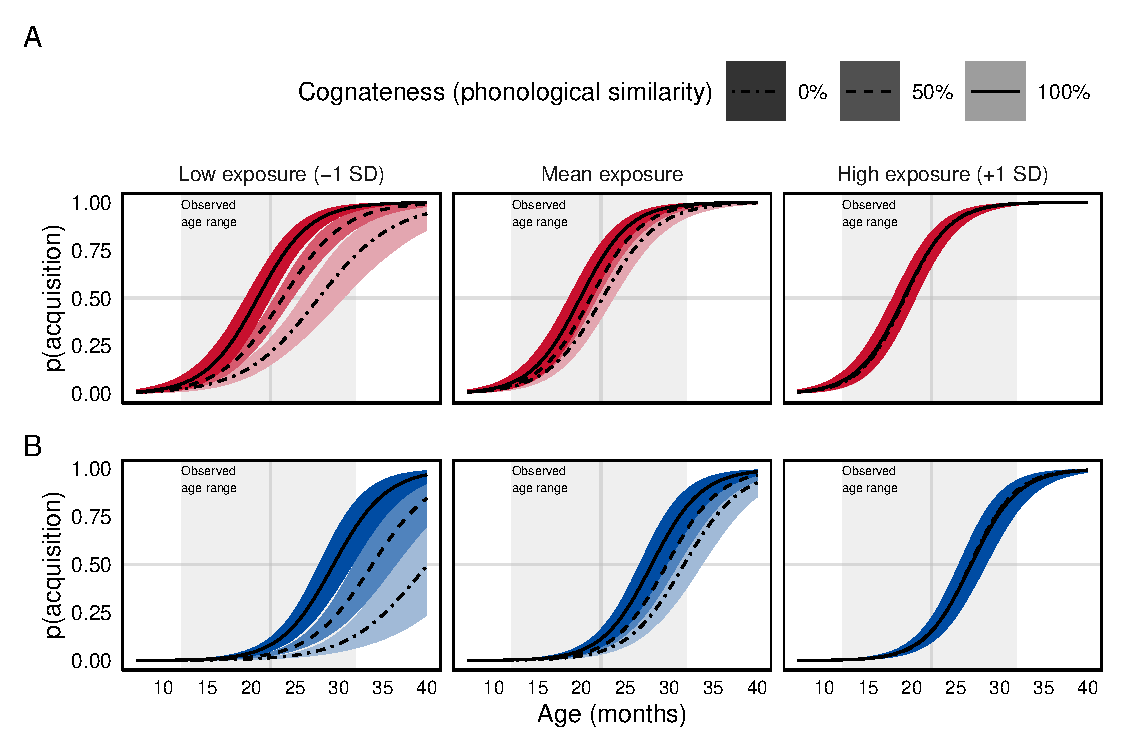
\includegraphics[width=1\textwidth,height=\textheight]{chapters/02-chapter-2_files/figure-pdf/fig-marginal-1.pdf}

}

\caption{\label{fig-marginal}Posterior marginal effects for
\emph{Comprehension} (A) and \emph{Production} (B). Lines and error
bands correspond to the mean and 95\% credible interval of the
posterior-predicted means. Different colour shades indicate different
levels of cognateness (phonological similarity). Predictions are
presented separately for different degrees of the word-form exposure
index: little exposure to the word-form, mean exposure, and high
exposure. In-sample predictions lie inside the grey rectangles. For
reference, we indicate the 50\% chance level of word acquisition
(horizontal grey lines), and the mean age of the sample (grey lines).}

\end{figure}

\elandscape

An additional analysis including lexical frequency and language exposure
as separate predictors (instead of the composite Exposure measure)
showed equivalent results (see Appendix B). To rule out the possibility
that cognateness facilitation effect we found was due to cognateness
comprising more frequent syllables than non-cognates---and therefore not
because of their cognate status itself---, we compared the syllabic
frequency of cognates and non-cognates included in our analyses. To
calculate syllable frequency, we first extracted all syllables embedded
in the selected words. For each syllable, we summed the lexical
frequency of all the words in which such syllable appeared. The
resulting value provided an estimate of the number of times the syllable
appears in child-directed speech, embedded within different words.
Finally, for each word-form, we summed the frequency of its syllables,
as an estimate of the syllabic frequency of the word-form. We fit a
Bayesian model with Cognateness as response variable, and the main
effects of syllable frequency and number of syllables (to control for
the fact words with more syllables are more likely to score higher in
syllabic frequency) as predictors. This model provided strong evidence
for the association between cognateness and syllabic frequency being
equivalent to zero (see Appendix C).

\hypertarget{sec-discussion}{%
\section{Discussion}\label{sec-discussion}}

This study investigated the impact of cognateness (i.e., phonological
similarity between translation equivalents) on the early bilingual
lexicon. We used Bayesian item response theory to model the acquisition
trajectories of a large sample of Catalan and Spanish words, estimating
the effect of cognateness on the probability of acquisition. This model
corrected for participants' age, word-form length (number of phonemes),
and a novel measure of participants' exposure rate to each word-form.
Exposure rates were calculated as a language exposure-weighted lexical
frequency score in which each word-form's lexical frequency was
corrected by the degree to which the participant was exposed to each
language. Overall, we found that cognates (i.e., phonologically similar
translation equivalents) were acquired earlier than non-cognates. This
effect was mediated by exposure rate. Low-exposure word-forms benefited
from their cognate status, whereas high-exposure word-forms did not.
Using the concept of accumulator (see Kachergis et al., 2022b for
review), we provide a theoretical account of bilingual lexical
acquisition. In the present account, parallel activation of the two
languages plays a central role during the acquisition of early
representations in the bilingual lexicon, and in which the dynamics of
co-activation between translation equivalents results in an earlier
age-of-acquisition.

The present investigation is particularly relevant in the light of two
previous findings. First, Floccia, Sambrook, Delle Luche, Kwok, Goslin,
White, Cattani, Sullivan, Abbot‐Smith, et al. (2018) reported that
bilingual toddlers learning two typologically close languages
(e.g.~shared many cognates, like English-Dutch) showed larger vocabulary
sizes than those learning typologically distant languages (e.g., shared
fewer cognates, like English-Mandarin). Second, Mitchell et al. (2022)
found an earlier age-of-acquisition for cognates, compared to
non-cognates. The outcomes of both studies pointed to cognateness
facilitating word acquisition through parallel activation, but the
underpinnings of such effect were unclear. While parallel activation has
been extensively described in experimental studies, current paradigms of
bilingual word acquisition and word learning are, to a large extent,
dissociated from the mechanisms proposed by previous work on word
processing. The notion of accumulator, as conceptualised by accumulator
models of language acquisition, may provide a convenient theoretical
framework to narrow this gap.

Accumulator models devise word acquisition as a continuous process in
which the child gathers information about words by accumulating learning
instances with such words. When the number of cumulative learning
instances for a word reaches some theoretical threshold, the child is
considered to have acquired such word. The rate at which a child
accumulates learning instances with a word is a function of child-level
properties (e.g., ability, amount of quantitative language exposure) and
word-level properties (e.g., lexical frequency) (Hidaka, 2013). Through
statistical inference, formalised accumulator models provide meaningful
information about parameters of interest like the aforementioned
predictors (Kachergis et al., 2022b; Mollica \& Piantadosi, 2017b), and
allow to generate quantitative predictions about age-of-acquisition and
vocabulary growth under competing theoretical accounts (Hidaka, 2013;
McMurray, 2007). Using the notion of accumulator, we extended this type
of account to the bilingual case. We suggested that the cognate
facilitation effect on bilingual word acquisition is the result of
cognate words being activated more strongly by their translation than
non-cognates. This would lead cognate words to accumulate learning
instances at a faster rate than non-cognate words. When a bilingual
child is exposed to a word-form, they activate not only its
corresponding lexical representation, but also the lexical
representation of its translation. The amount of co-activation that
spreads from the spoken word-form to its translation is proportional to
the amount of phonological similarity between both word-forms. Cognates
would receive more activation from their translation than non-cognates,
leading children to accumulate learning instances with cognate words at
a faster rate than with non-cognate words. As a result, lexical
representations of cognate words would consolidate at earlier ages than
those of non-cognate words.

These predictions address a critical subject in bilingualism research.
Do bilingual infants accumulate learning experiences in both languages
independently, or does exposure to one language impact the acquisition
trajectory of the other language? In the context of lexical acquisition,
the former scenario predicts that every learning instance for a given
word-form contributes to the acquisition of the representation of such
word in the lexicon, while the acquisition of its translation remains
unaffected by such experience. In the latter scenario, a learning
instance to the same word-form would contribute not only to the
acquisition of the representation of the word, but also, to some extent,
to the acquisition of its translation. Our findings provide strong
support for an account of bilingual vocabulary growth in which the
experience and learning outcomes accumulated by the child in one
language impact those in the other language through cross-language
phonological associations. Such a facilitatory mechanism might be an
important piece in the puzzle of bilingual language acquisition. In
particular, it may shed some light on why bilingual infants do not show
relevant delays in language acquisition milestones compared to their
monolingual peers, while receiving a reduced quantity of speech input in
each of their languages. Infants in the present study benefited more
strongly from the cognateness facilitation effect when acquiring words
from the language of lower exposure than in the language of higher
exposure.

This mechanism might be extended to provide a plausible explanation for
the language similarity facilitation reported by Floccia et al.~The
authors observed a facilitation in the additional (non-English)
language. Children learning two typologically close languages knew more
words in the additional language than those learning two typologically
more distant languages. In their sample, the additional language was
consistently also the lower-exposure language for most children, while
English was the higher-exposure language. Given that words in English
were more likely to be acquired first, higher phonological overlap for
words in the language of lower exposure (especially those of lower
lexical frequency) would facilitate vocabulary growth for languages
sharing more cognates with English.

The asymmetric facilitation of cognateness on word acquisition reported
in the present study parallels previous findings in toddlers and adults.
For instance, unbalanced (or low-proficiency) bilinguals benefit from
cross-language forward priming (dominant to non-dominant) during word
processing (De Groot \& Nas, 1991; Grainger, 1998; Shook \& Marian,
2019; Singh, 2014; Von Holzen et al., 2019b; but see Jardak \&
Byers-Heinlein, 2019). One the other hand, backward priming
(non-dominant to dominant) seems less robust and more challenging to
detect (e.g., Hoshino et al., 2010; Midgley et al., 2009; but see Duyck
\& Warlop, 2009). Balanced (or high-proficiency bilinguals) show an
equivalent priming facilitation in both directions (Basnight-Brown \&
Altarriba, 2007; Duñabeitia et al., 2009). These results have been taken
as evidence for an asymmetry in the strength of forward and backward
connections in the unbalanced bilingual lexicon. Although implemented in
different ways, or found under different assumptions, such a
dominance-mediated asymmetry is accounted for by multiple models of
lexical processing like the Revised Hierarchical Model (Kroll \&
Stewart, 1994), BIA/BIA+ (Dijkstra \& Van Heuven, 2013), BLINCS (Shook
\& Marian, 2013), or Multilink (Dijkstra et al., 2019), and also by
models providing a more development-oriented perspective, like the
Ontogenic Model (Bordag et al., 2022; Cook et al., 2016), and BIA-d
(Grainger et al., 2010). Overall, this provides an apparently convenient
account for the interaction between language dominance and cognateness
found in the present study. These models are aimed at explaining results
in adults, and their predictions should be taken with caution when
extended to early language acquisition.

In adult bilingual populations, language dominance and proficiency are
frequently defined using dimensions other than degree of exposure, which
is a more common practice in infant research (Marian \& Hayakawa, 2021;
Rocha-Hidalgo \& Barr, 2023a). For instance, low-proficiency bilinguals
in many of the aforementioned studies acquired their second language
years after their toddlerhood. We identify three critical ways in which
this prevents a clear comparison between our results and those from
studies on second language acquisition in adults. First, in adult second
language acquisition, the acquisition of the phonology of the new
language must be negotiated with the already acquired phoneme inventory
of the first language (e.g., Cutler et al., 2006; Sebastian-Gallés et
al., 2006), in place around the first year of life (see Werker \&
Hensch, 2015 for review). Second, adults acquiring a second language
already possess a system of form-meaning mappings, whereas simultaneous
bilingual infants must build a lexicon for two languages in the absence
of clear form-meaning mappings. Third, adults are assumed to be literate
and to possess an orthographic system in place, which may shape how new
words are integrated in the lexicon and processed during experimental
tasks (e.g., Thierry \& Wu, 2007). In this scenario, the acquisition of
a second language may take place in a substantially different way
compared to how bilingual infants acquire two languages from birth. A
more similar case to the one concerning the present study is considered
by the DevLex-II model (Zhao \& Li, 2010), which captures unique
features of the early bilingual lexicon, and considers the case of
infants simultaneously acquiring their two language. In line with the
adult models, DevLex-II predicts asymmetries between word representation
from the dominant and the non-dominant language. Simulations from
DevLex-II result in an asymmetric cross-language priming, in which words
from the dominant (acquired acquired) language primed more strongly the
recognition of words in the non-dominant language (later acquired) than
in the other direction (Zhao \& Li, 2013).

In summary, there is a compelling case for attributing asymmetric
effects of parallel activation to differences in activation strength
between forward and backward connections. It is nonetheless possible
that, as argued in the introduction, the asymmetric effect of
cognateness found in the present study is simply the result of infants
being exposed more frequently to words in the dominant language than to
words in the non-dominant language. This would lead to words in the
non-dominant language receiving additional parallel activation, compared
to words in the dominant language, and therefore benefiting more
strongly from their cognate status. These two accounts are not mutually
exclusive, as words in the dominant language may active more strongly
their translations than vice versa, on top of such activation being more
frequent. Further research is needed in order to clarify this issue.

It might be argued that our results reflect the fact that cognate
translation equivalents are represented in the initial bilingual lexicon
as the same lexical entry. Because cognates correspond to similar
sounding word-forms in equivalent referential contexts (e.g., hearing
/\textipa{"gat}/ and /\textipa{"ga.to}/ in the same situations), it is
possible that infants classify both are as acceptable variations of the
same word-form, therefore treating them as a single lexical item. This
would lead to a faster increase in cumulative learning instances, and to
an earlier age-of-acquisition for cognate translation equivalents (for
which listening to each word-form contributes to the acquisition of its
shared representation), compared to non-cognates (for which listening to
each word-form contributes to the acquisition of a separate
representation). This mechanism could potentially explain the earlier
age-of-acquisition effect of cognates found in the present study,
without the need of parallel activation playing any relevant role.
Mitchell et al. (2022) discuss this possibility as a candidate
explanation of the cognate facilitation effect, in which bilinguals only
need to map one word-form to the referent in the case of cognates, while
mapping two distinct word-forms in the case of non-cognates. However,
previous work on mispronunciation perception and learning of minimal
pair words points in a different direction. Bilingual toddlers show
monolingual-level sensitivity to slight phonetic changes in a word-form,
according to their performance in word recognition tasks (Bailey \&
Plunkett, 2002; Mani \& Plunkett, 2011b; Ramon-Casas et al., 2009b,
2017; Ramon-Casas \& Bosch, 2010; Swingley, 2005b; Swingley \& Aslin,
2000; Tamási et al., 2017; Wewalaarachchi et al., 2017). The ability to
differentiate between similar-sounding word-forms is also reflected in
word learning, as bilinguals seem to be able to map minimal pairs to
distinct referents (Havy et al., 2016; Mattock et al., 2010; Ramon-Casas
et al., 2017). Overall, it seems that bilinguals consider small
differences in the phonological forms of words as relevant at the
lexical level. We argue that this shows evidence that bilingual toddlers
likely form distinct lexical representations for even near-identical
cognates.

Our study shares similar methodological limitations with previous work
using vocabulary reports provided by caregivers. Such reports can be
subject to measurement error induced by caregivers who may sometimes
overestimate or underestimate participants' true probability of word
acquisition (e.g., Houston-Price et al., 2007). In the case of bilingual
research additional biases may be in place. Although in the present
study caregivers were explicitly instructed not to rely on their
responses to Catalan words when responding to Spanish (and vice versa),
it is possible that some caregivers assumed---at least to some
extent---that because the child knew a word in one language, the child
should also know the word in the other language. This bias would
especially affect similar-sounding words, i.e., cognates. Production
estimates may be more prompt to such biases, in part because of the
slower pace at which infants' articulatory abilities develop, compared
to their word recognition abilities (Hustad et al., 2021). This gap
between comprehension and production is even larger in the less dominant
language of bilingual children (Giguere \& Hoff, 2022). For this reason,
caregivers may be more uncertain about what words can be counted as
acquired in this modality. Despite such potential biases, vocabulary
checklist filled by parents show strong evidence of concurrent validity
with other estimates of vocabulary size or lexical processing (Feldman
et al., 2005; Gillen et al., 2021; but see Houston-Price et al., 2007).

The present study contributes with a specific data point to the complex
landscape of bilingualism research. Bilinguals are a remarkably
heterogeneous population difficult to be satisfactorily characterised in
a comprehensive way (Sebastian-Galles \& Santolin, 2020b). Bilinguals
differ across multiple dimensions. Such differences span from
exclusively linguistic factors; such as the amount of overlap between
the phonemic inventories of the two languages being learned (e.g., low,
like the case of English and Mandarin, or high, like the case of Spanish
and Greek), to extralinguistic factors like the sociolinguistic
situation in which the two languages co-exist (e.g., in some regions
both languages are co-official and used in similar contexts, while in
others, one of the languages has a smaller societal presence, i.e.,
heritage languages). This diversity of situations in which bilingual
toddlers acquire language calls for special consideration of the
generalisability of results in bilingualism research. Our sample,
although homogeneous (e.g., similar parental educational level across
participants), represents a particular bilingual sociolinguistic
environment. The languages involved in the present investigation,
Catalan and Spanish, co-exist in Catalonia as official languages, both
languages are used in fairly similar contexts, and both languages are
known by the majority of the population. In 2018, more than 81.2\% of a
representative sample of 8,780 adults aged 15 years or older living in
Catalonia reported being able to speak Catalan, and more than 99.5\% of
the same population reported being able to speak Spanish (\emph{Els Usos
Lingüístics de La Població de Catalunya}, 2018). In addition, Catalan
and Spanish are Romance languages and share a considerable amount of
cognates. Extending our analyses to other bilingual populations learning
typologically more distant languages, and whose languages tend to be
used in more distinct contexts (e.g., heritage languages) should be a
natural future step for the present investigation.

To conclude, our study provides novel insights about word acquisition in
bilingual contexts, and how the presence of cognates in the children's
linguistic input impacts the early formation of the lexicon. We found
that during the acquisition of low frequency words, bilingual children
seem to benefit more strongly from the word-form's phonological
similarity with its translation in the other language. Capitalising on
the notion of accumulator of linguistic input, we put forward a
theoretical account of bilingual word learning, in which cognateness
interacts with lexical frequency and language exposure to boost the
acquisition of translation equivalents.

\hypertarget{appendix-a-model-details}{%
\section{Appendix A: Model details}\label{appendix-a-model-details}}

\textbf{Model structure and prior}. We used Stan (Carpenter et al.,
2017) as the probabilistic language behind the estimation of our
Bayesian models in this study, with \texttt{brms} as its R interface
(Bürkner, 2017). This language implements the Markov Chain Monte Carlo
(MCMC) algorithm using the Hamiltonian Monte Carlo method (HMC) to
explore the posterior distribution of the model. Broadly, this algorithm
is used to iteratively sample the joint sampling space of the parameters
to be estimated in the model, and compute, for each value sampled, its
likelihood under some probability distribution previously defined. We
run four MCMC chains, each 1,000 iterations long each.

\textbf{Considerations on statistical power and sample size}. There is
little consensus about what approach is adequate for calculating the
statistical power of a complex Bayesian model like the one in the
present study, for several reasons. A first pitfall, shared with
frequentist analysis, is that a closed solution for statistical power
calculation is not possible or cannot be computed within reasonable time
constraints. This rules out the use of many available pieces of software
that are commonly offered for power analysis, as they commonly only
consider the case of simpler models like t-tests, ANOVA, Pearson
correlation, or regression (with only fixed effects), or trivial
derivations of thereof. The more complicated case of multilevel models
is usually not covered, not to mention those with a Bayesian approach.

An alternative way of estimating the statistical power of statistical
test is simulation. This consists on simulating multiple datasets in
which the hypothesised effect size is present, and fitting multiple
instances of the model. The statistical power is derived from the
proportion of contrasts that result in the rejection of the null
hypothesis across datasets. Although this approach permits the
estimation of statistical power in the case of more complex models, it
involves costly computations. In the case of Bayesian models, and
particularly the one in the present study, such cost can be infeasible.
Sampling the posterior of our model took approximately seven days.
Running this model, or an equivalent one, across 100 datasets (100 may
even be considered too few by many) would take more than a year.

Following J. Kruschke (2014), we considered the precision of our
estimates as a proxy to statistical power. In particular, we compared
the width of the 95\% HDI of the critical regression coefficient
(\emph{Exposure} \(\times\) \emph{Cognateness}) against some nominal
interval width. We decided to use the half the width of the ROPE in the
logit scale {[}-0.025, +0.025{]}, that is, 0.05 as the reference
interval width. The width of the fixed regression coefficient of
\emph{Exposure} \(\times\) \emph{Cognateness} (\(\beta\) = -0.014, 95\%
HDI = {[}-0.017, -0.011{]}) was 0.006, around 8.933 times narrower than
the reference interval. This indicates that the precision of the
posterior 95\% HDI of the critical parameter in the model is larger than
required.

\textbf{Model diagnostics}. One way to diagnose the behaviour of the HMC
algorithm is to inspect whether the different MCMC chains (if more than
one) have converged to a similar region of the posterior. The
Gelman-Rubin diagnostic (\(\hat{R}\) or R-hat Gelman \& Rubin, 1992)
provides a measure of chain convergence by comparing the variance within
each chain \emph{versus} the variance between each chain. Both are
expected to be identical when chains have perfectly converged, so that
\(\hat{R} = 1\). Values lower than 1.01 are recommended, while values
higher than 1.05 indicate that chains might have trouble converging and
therefore the estimated parameters must be taken with caution.
Figure~\ref{fig-rhats-neffs} (A) shows the distribution of \(\hat{R}\)
values for the coefficients of the fixed effect of our models, which we
used for statistical inference. Most values are lower than 1.01, and
never higher than 1.05, which provides evidence of successful MCMC
convergence.

Another diagnostic of good MCMC converge is the ratio of effective
sample size to total sample size (\(N_{eff}/N\)), which indicates the
proportion of samples in the chain that resulted from a non-divergent
transition. Values closer to 1 are ideal, as they indicate that all
posterior samples from the MCMC were used to estimate the posterior
distribution of the parameter. Values larger than 0.1 are recommended.
Figure~\ref{fig-rhats-neffs} (B) shows the distribution of the effective
sample sizes of the coefficients of the fixed effects in our models.
Most values are larger than 0.1, although model 0 (\(\mathcal{M}_0\))
accumulates most effective sample sizes close to 0.1.

Another way of assessing the behaviour of the HMC algorithm is to
visualise the joint posterior distribution for pairs of parameters using
bi-variate scatter plots. In Figure~\ref{fig-model-pairs} we show the
pair-wise distribution of posterior samples. Broadly, posterior samples
of two parameters should not be correlated. This is the case for all
pairs of parameters but for the two intercepts. This is expected
behaviour, given that these two parameters correspond to the thresholds
between categories in the ordinal regression model, and the distance
between both thresholds is fixed in the particular parametrisation of
the model.

\newpage

\blandscape

\begin{figure}

{\centering 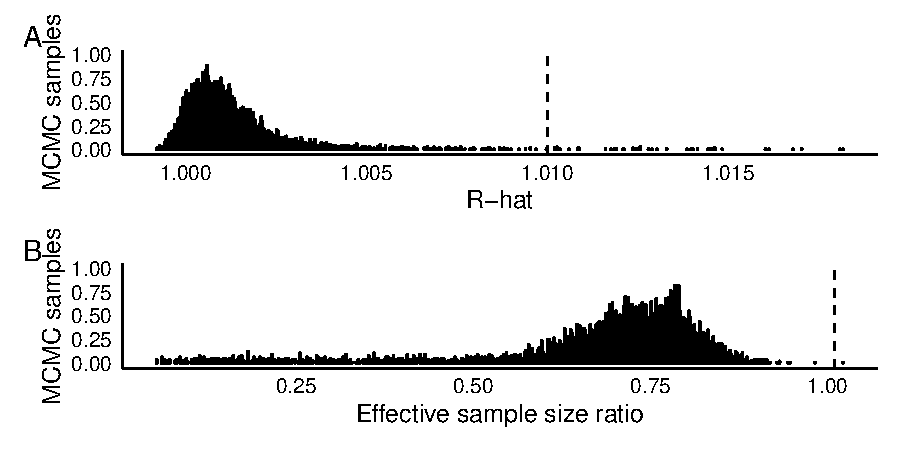
\includegraphics{chapters/02-chapter-2_files/figure-pdf/fig-rhats-neffs-1.pdf}

}

\caption{\label{fig-rhats-neffs}MCMC convergence diagnostic of all
parameters in the model. Each dot represents the score of one parameter.
(A) Distribution of the Gelman-Rubin (R-hat) scores. (B) Distribution of
the ratio of effective sample size.}

\end{figure}

\elandscape

\newpage

\blandscape

\begin{figure}

{\centering 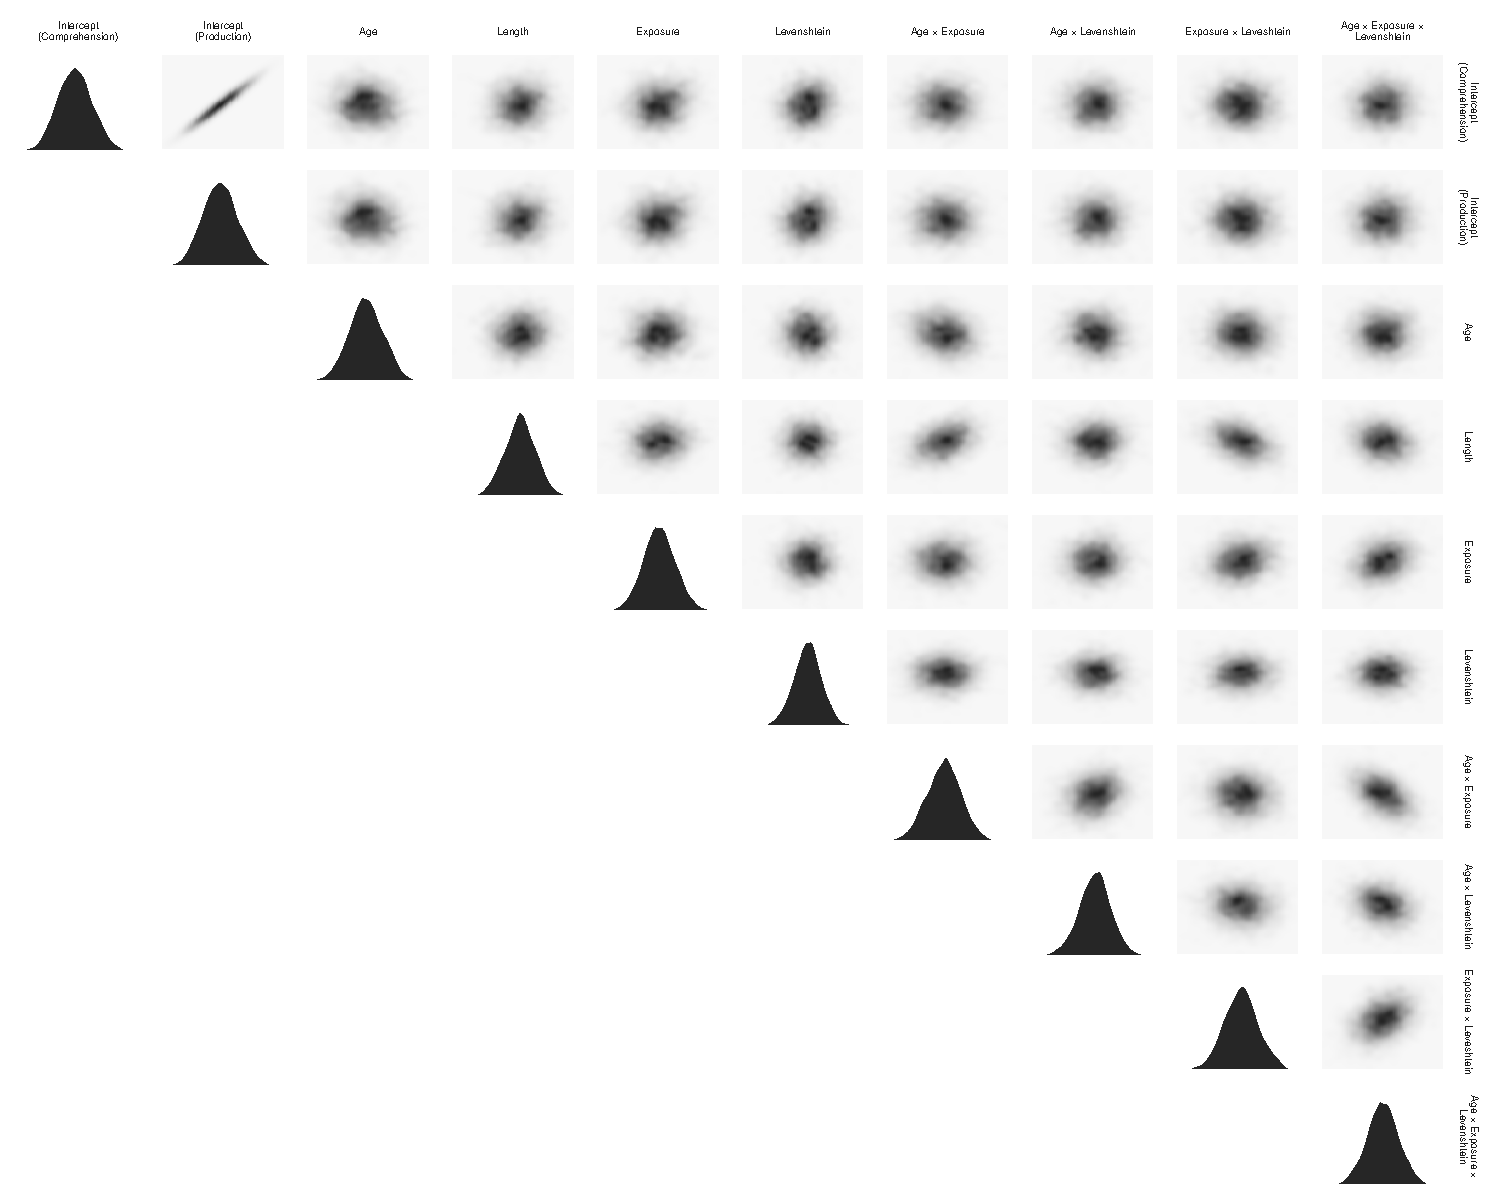
\includegraphics{chapters/02-chapter-2_files/figure-pdf/fig-model-pairs-1.pdf}

}

\caption{\label{fig-model-pairs}Marginal distribution and bi-variate
scatterplot of posterior samples for the fixed regression coefficients
in the model.}

\end{figure}

\elandscape

\newpage{}

\hypertarget{appendix-b-frequency-and-language-exposure-as-separate-predictors}{%
\section{Appendix B: Frequency and language exposure as separate
predictors}\label{appendix-b-frequency-and-language-exposure-as-separate-predictors}}

As a robustness check, we fit a model similar to the one described in
the main manuscript, but including lexical frequency and language degree
of exposure as separate predictors, instead of the composite measure
\emph{Exposure}. Language degree of exposure (\emph{DoE}) was included
in interaction with \emph{Age} and \emph{Cognateness}, while lexical
frequency (\emph{Frequency}) was included as a main effect.
Table~\ref{tbl-coefs-doe} shows a comparison between the posterior
distribution of the regression coefficients of both models. Overall,
results are equivalent. \newpage

\blandscape

\hypertarget{tbl-coefs-doe}{}
\begin{table}
\caption{\label{tbl-coefs-doe}Posterior distribution of regression coefficients of the model including
the \emph{Exposure} composite predictor, and of the model including
lexical frequency (\emph{Frequency}) and degree of exposure (\emph{DoE})
separately. \(\beta\): median of the posterior distribution in the
probability scale. 95\% HDI: 95\% highest density interval of the
distribution. \(p(\text{ROPE})\): overlap between the 95\% HDI and the
ROPE, indicating the posterior probability that the true value of the
coefficient is equivalent to zero. }\tabularnewline

\centering
\begin{tabular}{lclr}
\toprule
 & $\beta$ & 95\% HDI & $p(\text{ROPE})$\\
\midrule
\addlinespace[0.3em]
\multicolumn{4}{l}{\textbf{Model: Exposure}}\\
\hspace{1em}Length (+1 SD, 1.56 phonemes) & 0.485 & {}[0.478, 0.491] & .000\\
\hspace{1em}Age (+1 SD, 4.87 months) & 0.600 & {}[0.588, 0.611] & .000\\
\hspace{1em}Exposure (+1 SD, 1.81) & 0.558 & {}[0.549, 0.566] & .000\\
\hspace{1em}Cognateness (+1 SD, 0.26) & 0.514 & {}[0.504, 0.526] & .102\\
\hspace{1em}Exposure $\times$ Cognateness & 0.486 & {}[0.483, 0.489] & .000\\
\hspace{1em}Age $\times$ Exposure & 0.518 & {}[0.51, 0.526] & .000\\
\hspace{1em}Age $\times$ Cognateness & 0.504 & {}[0.5, 0.507] & .928\\
\hspace{1em}Age $\times$ Exposure $\times$ Cognateness & 0.495 & {}[0.493, 0.497] & .908\\
\addlinespace[0.3em]
\multicolumn{4}{l}{\textbf{Model: Frequency \& DoE}}\\
\hspace{1em}Age (+1 SD, 4.87, months) & 0.600 & {}[0.59, 0.612] & .000\\
\hspace{1em}Phonemes (+1 SD, 1.56 phonemes) & 0.486 & {}[0.48, 0.492] & .000\\
\hspace{1em}Frequency (+1 SD, 0.19) & 0.527 & {}[0.516, 0.539] & .000\\
\hspace{1em}DoE (+1 SD, 0.3) & 0.557 & {}[0.549, 0.566] & .000\\
\hspace{1em}Cognateness (+1 SD, 0.26) & 0.516 & {}[0.505, 0.527] & .064\\
\hspace{1em}Age $\times$ DoE & 0.518 & {}[0.51, 0.526] & .000\\
\hspace{1em}DoE $\times$ Cognateness & 0.486 & {}[0.483, 0.488] & .000\\
\hspace{1em}Age $\times$ Cognateness & 0.504 & {}[0.501, 0.507] & .852\\
\hspace{1em}Age $\times$ DoE $\times$ Cognateness & 0.495 & {}[0.493, 0.497] & .900\\
\bottomrule
\end{tabular}
\end{table}

\elandscape

\newpage{}

\hypertarget{appendix-c-syllable-frequency}{%
\section{Appendix C: Syllable
frequency}\label{appendix-c-syllable-frequency}}

We define syllable frequency as the rate of appearance of individual
syllables in the word-forms included in the Barcelona Vocabulary
Questionnaire (BVQ) (Garcia-Castro, Ávila-Varela, et al., 2023a). Each
item corresponds to a Catalan or Spanish word, and has an associated
phonological transcription in X-SAMPA format (Wells, 1995). These
transcriptions are syllabified. Some examples:

\newpage

\blandscape

\hypertarget{tbl-syll-items}{}
\begin{table}
\caption{\label{tbl-syll-items}Sample of items included in the BVQ questionnaire and their syllabified
SAMPA transcriptions in Catalan and Spanish. }\tabularnewline

\centering
\begin{tabular}{lllcllc}
\toprule
Translation & Item & X-SAMPA & Syllables & Item & X-SAMPA & Syllables\\
\midrule
white & blanc & b5aN & 1 & blanco & "blan.ko & 2\\
ham & pernil & p@r"ni5 & 2 & jamón (york) & "xa"mon & 2\\
knee & genolls & Z@"noLs & 2 & rodillas & ro"Gi.Las & 3\\
stairs & escalaes & @s"ka.5@s & 3 & escaleras & eska"le.4as & 3\\
candy & caramel & k@.4@"mE5 & 3 & caramelo & ka.4a"me.lo & 4\\
\addlinespace
orange (food) & taronja & "t4OJ.Z@ & 2 & naranja & na"4an.xa & 3\\
turtle & tortuga & tur"tu.G@ & 3 & tortuga & to4"tu.Ga & 3\\
strawberry & maduixa & m@"Du.S@ & 3 & fresa & "f4e.sa & 2\\
park & parc & park & 1 & parque & "pa4.ke & 2\\
uncle & oncle & "oN.k5@ & 2 & tío & "ti.o & 2\\
\addlinespace
cookie & galeta & g@"5E.t@ & 3 & galleta & ga"Le.ta & 3\\
zipper & cremallera & k4@.m@"Le.4@ & 4 & cremallera & k4e.ma"Le.4a & 4\\
syrup & xarop & S@"4Op & 2 & jarabe & xa"4a.Be & 3\\
book & llibre & "Li.B4@ & 2 & libro & "li.B4o & 2\\
yard & jardí & Z@r"Di & 2 & jardín & xa4"Din & 2\\
\bottomrule
\end{tabular}
\end{table}

\elandscape

Most Catalan and Spanish words had two syllables, with Spanish words
having three and four syllables more often than Catalan words. Less than
1\% of the words included in the analyses presented in the main body of
the manuscripts had five syllables. No words had more than five
syllables (see Figure~\ref{fig-syll-number}). We extracted lexical
frequencies from the English corpora in the CHILDES database
(MacWhinney, 2000; Sanchez et al., 2019a). Using the Catalan and Spanish
corpora was not possible due to the low number of children and tokens
included in the corpora.

\begin{figure}

{\centering 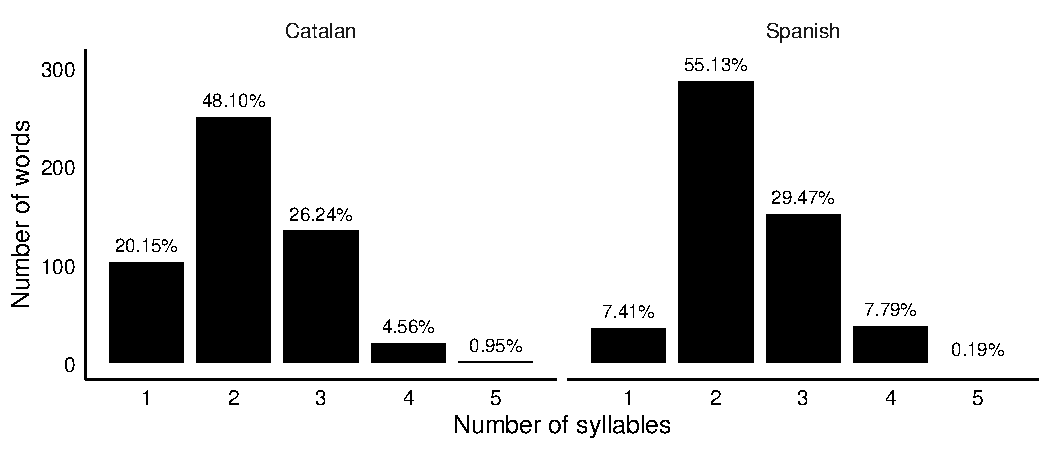
\includegraphics{chapters/02-chapter-2_files/figure-pdf/fig-syll-number-1.pdf}

}

\caption{\label{fig-syll-number}Distribution of the number of syllables
in Catalan and Spanish}

\end{figure}

We now present how syllable frequencies were calculated. Every exposure
to a word-form also counts as a exposure to each of the syllables that
make up such word. Every time a child hears the word \emph{casa}
{[}house{]}, they are exposed to the syllables \emph{ca} and \emph{sa}.
Syllables that appear embedded in words with higher lexical frequency
will also be more frequent. To compute the relative frequency of each
syllable in Catalan and Spanish (i.e., how many times the syllables
appears in every million words in Catalan or Spanish speech), we summed
the relative lexical frequency in CHILDES of every word that contains
such syllable in the corresponding language. Figure~\ref{fig-syll-freq}
shows the distribution of frequencies across syllables in Catalan and
Spanish. In the log10 scale, syllable frequencies in Catalan and Spanish
followed a slightly asymmetric distribution, with most syllables scoring
around 1,000 counts per million, and a longer tail to the right of the
distribution.

\begin{figure}

{\centering 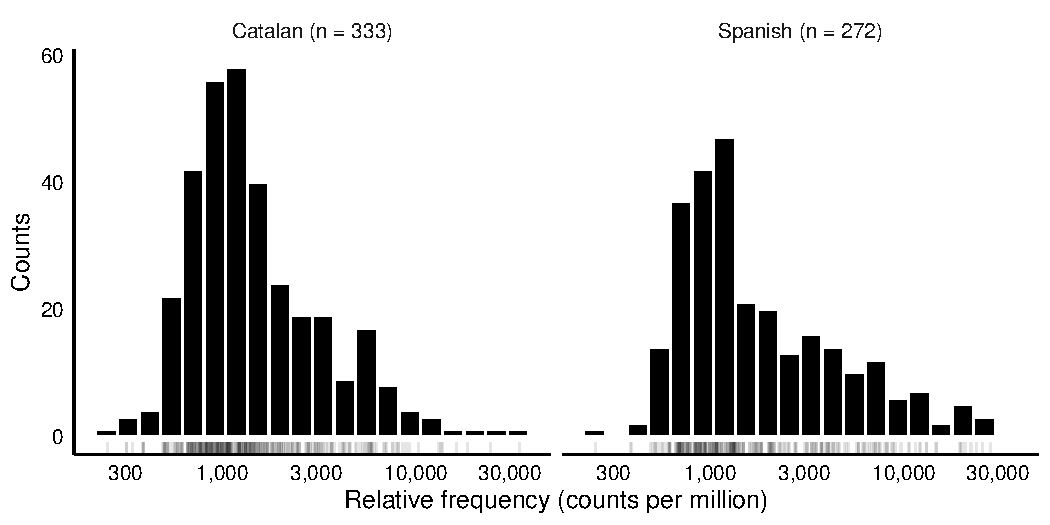
\includegraphics{chapters/02-chapter-2_files/figure-pdf/fig-syll-freq-1.pdf}

}

\caption{\label{fig-syll-freq}Distribution of apositional syllable
frequencies in Spanish and Catalan}

\end{figure}

To estimate the association between word-level syllabic frequency and
cognateness, while controlling for the number of syllables in the word,
(an increment in the number of syllables necessarily increases the
summed syllabic frequency of the word), we fit a multilevel, Bayesian
linear regression model with syllabic frequency (the sum of the syllabic
frequency of the syllables in a word) as response variable, and the main
effect of the number of syllables (\(Syllables\)) and \(Cognateness\)
(Levenshtein similarity between a word and its translation equivalent,
Levenshtein, 1966) as predictors. We added translation equivalent-level
random effects for the intercept and the main effect of \(Syllables\)
(some translation pairs had a different number of syllables in each
language). We used a Gaussian distribution to model syllabic frequency
scores after standardising this variable and the predictors. We used a
weakly informative prior for all parameters involved in the model (see
Equation~\ref{eq-model-syllables} for a formal equation of this model
and its prior). We conducted statistical inference by evaluating the
proportion of the 95\% highest density interval (HDI) of the posterior
posterior distribution of each coefficient that fell into the region of
practical equivalence (ROPE, see the main manuscript for a more detailed
explanation, J. K. Kruschke \& Liddell, 2018).

\begin{equation}\protect\hypertarget{eq-model-syllables}{}{
\begin{aligned}
y &\sim \mathcal{N}(\mu, \sigma)\\
\mu &= (\beta_0 + u_{0_{i}}) + (\beta_1 + u_{1_{i}}) \text{Syllables} + \beta_2 \text{Cognateness} \\
\beta_{0-3} &\sim \mathcal{N}(0, 10) \\
u_{{0-1}_{i}} &\sim \mathcal{N}(0, \sigma_{u_i}) \\
\sigma_y & \sim \text{Exponential}(2)\\
\sigma_{u_{0-1}} &\sim \mathcal{N_{+}}(1, 0.1) \\
\rho_{u} &\sim \text{LKJcorr}(2) \\
\end{aligned}
}\label{eq-model-syllables}\end{equation}

We fit this model running 4 sampling chains with 1,000 iterations each.
Table~\ref{tbl-syll-coefs} shows a summary of the posterior distribution
of the fixed effects in the model. As expected, words with more
syllables scored higher in syllabic frequency: all posterior draws for
the regression coefficient of the main effect of this predictor fell
outside the ROPE defined between -0.5 and +0.5 (\(\beta\) = 5.64, 95\%
HDI = {[}5.58, 5.71{]}). Keeping the number of syllables constant, the
effect of cognateness was negligible: all of the posterior distributions
of this predictor fell within the ROPE, providing evidence that the true
value of the increment in syllabic frequency for every increase in
cognateness is equivalent to zero (\(\beta\) = 0.01, 95\% HDI =
{[}-0.06, 0.08{]}).

\hypertarget{tbl-syll-coefs}{}
\begin{table}
\caption{\label{tbl-syll-coefs}Posterior distribution of regression coefficients. \(\beta\): median of
the posterior distribution in the probability scale. 95\% HDI: 95\%
highest density interval of the distribution. \(p(\text{ROPE})\):
overlap between the 95\% HDI and the ROPE, indicating the posterior
probability that the true value of the coefficient is equivalent to
zero. }\tabularnewline

\centering
\begin{tabular}{lclr}
\toprule
 & $\beta$ & 95\% HDI & $p(\text{ROPE})$\\
\midrule
Intercept & 16.090 & {}[16.022, 16.162] & NA\\
Syllables (+1 SD, 0.802) & 5.644 & {}[5.575, 5.713] & .000\\
Cognateness (+1 SD, 0.24) & 0.009 & {}[-0.056, 0.081] & 1.000\\
\bottomrule
\end{tabular}
\end{table}

Figure~\ref{fig-syll-marginal} shows the median posterior-predicted
syllabic frequencies for words with one to four syllables, for the whole
range of cognateness values. Overall, cognate words' syllabic frequency
is equivalent to that of non-cognates. This suggests that the cognate
facilitation effect in word acquisition reported in the present study is
not the result from an association between cognateness and higher
syllabic frequencies.

\newpage

\blandscape

\begin{figure}

{\centering 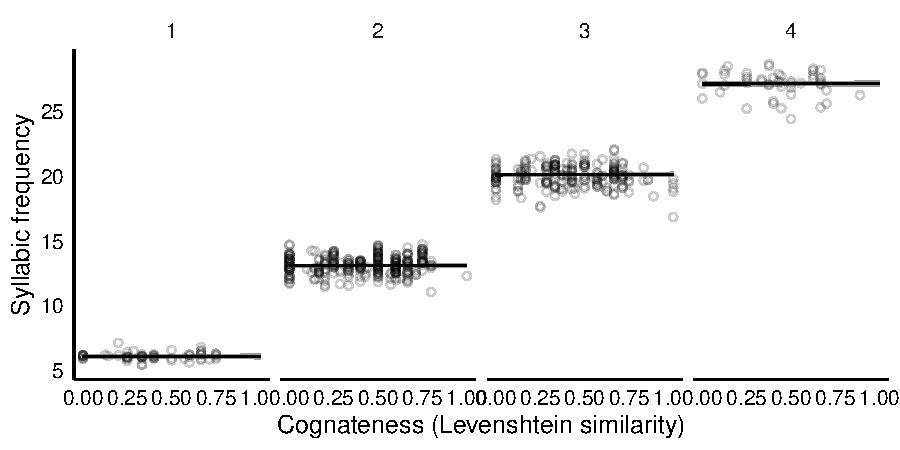
\includegraphics{chapters/02-chapter-2_files/figure-pdf/fig-syll-marginal-1.pdf}

}

\caption{\label{fig-syll-marginal}Posterior-predictions of the syllabic
frequency model. Thicker lines indicate the median of the posterior
predictions, and thinner lines indicate individual posterior
predictions.}

\end{figure}

\elandscape

\newpage{}

\bookmarksetup{startatroot}

\hypertarget{chapter-3-developmental-trajectories-of-langugage-non-selectivity-in-the-bilingual-lexicon}{%
\chapter{Chapter 3: Developmental trajectories of langugage
non-selectivity in the bilingual
lexicon}\label{chapter-3-developmental-trajectories-of-langugage-non-selectivity-in-the-bilingual-lexicon}}

\hypertarget{introduction-2}{%
\section{Introduction}\label{introduction-2}}

Building a mental lexicon is a major achievement in the development of
an infant: by storing representations of how familiar words sound and
what they mean, an infant is able to make sense of their linguistic
input. The foundations of an initial lexicon are in place before the end
the first year of life (Bergelson \& Swingley, 2012a, 2015; Hallé \&
Boysson-Bardies, 1994; Parise \& Csibra, 2012; Tincoff \& Jusczyk,
1999a; M. Vihman, 2004). This initial lexicon consists of only a few
items; mainly words for people, interjections, body parts, and food
(Tardif et al., 2008; Tincoff \& Jusczyk, 2012), but it undergoes rapid
growth during the second year of life (Bergelson, 2020; Bloom, 2002;
Ganger \& Brent, 2004; Goldfield \& Reznick, 1990; McMurray, 2007).
According to parental reports, the average 15-month-old infant already
understands more than 100 words, and by two years of age, they
understand more than 400 (Frank et al., 2021). This accelerated lexical
developmental is reflected in infants' trajectories of word recognition:
infants recognise familiar words faster and more efficiently as they
approach their second birthday (Fernald et al., 1998, 2001; Hurtado et
al., 2007). Despite being exposed to a more complex linguistic input,
bilinguals show equivalent trajectories of word acquisition and word
recognition to their monolingual peers' (Bialystok, 2009; Byers-Heinlein
et al., 2023b; De Houwer et al., 2014; Hoff et al., 2012; Legacy et al.,
2018; Pearson \& Fernández, 1994; Vihman et al., 2007). This is a
remarkable deed for two reasons. First, bilingual infants receive a
relatively reduced linguistic input in each of their languages, compared
to monolinguals (Cattani et al., 2014; Costa \& Sebastián-Gallés, 2014;
Thordardottir, 2011). Second, they face a more complex referential
context: they often learn two labels for each referent (one in each
language), which additionally may not be direct translations of each
other (Au \& Glusman, 1990; Bilson et al., 2015; De Houwer et al., 2006;
R. K.-Y. Tsui et al., 2022a). The mechanisms that allow bilingual'
trajectories of lexical developmental to keep up with monolinguals' are
still unclear.

Previous studies have pointed to the similarity between the two
languages of exposure as a facilitator of lexical acquisition in
bilinguals (Blom et al., 2020a; Floccia, Sambrook, Delle Luche, Kwok,
Goslin, White, Cattani, Sullivan, Abbot-Smith, et al., 2018; Gampe et
al., 2021). Floccia, Sambrook, Delle Luche, Kwok, Goslin, White,
Cattani, Sullivan, Abbot-Smith, et al. (2018) reported larger vocabulary
sizes in bilingual toddlers leaning two languages that shared high
lexical similarity. The authors collected parental reports of vocabulary
data from a sample of 367 bilingual children living in the United
Kingdom, who were learning English and an additional language (out of a
diverse pool of 13 languages). The authors then calculated the average
phono-lexical similarity between English and each of the additional
languages. English and Dutch shared the highest similarity, while
English and Mandarin shared the lowest. Overall, children's vocabulary
sizes in the additional language was positively associated with the
amount of language similarity between their two languages. For instance,
English-Dutch bilinguals showed larger vocabulary sizes in Dutch than
English-Mandarin bilinguals did in Mandarin. The authors suggested that
the acquisition of words in the additional language might be facilitated
by their cognate status (i.e., being phonologically similar to their
translation equivalent). If this is the case, larger vocabulary sizes
might then be expected in bilinguals learning two languages sharing a
high proportion of cognates. This would be consistent with available
evidence of an earlier acquisition of cognate words (Bosch \&
Ramon-Casas, 2014; Garcia-Castro, Avila-Varela, et al., 2023; Mitchell
et al., 2022; Schelletter, 2002).

The facilitation effect of cognateness is in line with the language
non-selective account of bilingual lexical access. This account proposes
that bilinguals activate both languages in parallel, even during
monolingual situations. In adults, there is robust evidence in favour of
this language non-selective account of lexical access (Dijkstra et al.,
1999, 2010; Dufour \& Kroll, 1995; Groot, 1992; Marian \& Spivey, 1999;
Schwartz et al., 2007; Spivey \& Marian, 1999). Costa et al. (2000)
presented highly-proficient Catalan-Spanish bilinguals with a series of
pictures of familiar objects. Participants were asked to name each
picture in Spanish. Unbeknownst to participants, the authors manipulated
the cognate status pictures' labels in Catalan and Spanish. In half of
the trials, the labels associated to the pictures were cognates (e.g.,
\emph{cat}-\emph{gat} {[}cat{]}), whereas in the other half of the
trials the labels were non-cognates (e.g., \emph{taula}-\emph{mesa}
{[}table{]}). Participants named pictures faster in cognate trials than
in non-cognate trials. Spanish monolinguals showed equivalent naming
times in both conditions. These results revealed that bilinguals
activated their Catalan phonology, despite performing the naming task
exclusively in Spanish: the visual recognition of the presented pictures
led to the parallel activation of its associated phonological forms in
both languages, which influenced the subsequent dynamics of word
production.

Parallel activation has also been reported in the developing lexicon
(Bosma et al., 2019; Bosma \& Nota, 2020; Floccia et al., 2020; Jardak
\& Byers-Heinlein, 2019; Poarch \& Van Hell, 2012; Singh, 2014; Von
Holzen et al., 2019a). Von Holzen \& Mani (2012a) found evidence of
cross-language phonological priming in a sample of 20 German-English
bilinguals aged 21 to 43 months. In their experimental task, each trial
begun with the auditory presentation of an English prime word, followed
by a target word in German, and a pair of target and distractor
pictures. The authors recorded participants' target picture looking as a
measure of target word recognition. The authors manipulated the
cross-linguistic phonological overlap between the prime and the target
labels. In a \emph{priming through translation} condition, the English
prime labels (leg) did not overlap with the German target labels
(\emph{Stein} {[}stone{]}), but with their German translations
(\emph{Bein}) did. In the \emph{unrelated} condition, prime and target
labels were not phonologically related in either German or English. If
participants accessed their lexicon in a language non-selective way, the
auditory presentation of the prime label in English should lead to the
co-activation of its German translation. If this is the case, target
word recognition should be interfered by the prior activation of a
phonologically related German prime label. Under this hypothesis, the
authors anticipated an delayed target looking in priming through
translation trials, compared to unrelated trials. The results supported
this hypothesis. In spite of the relevance of Von Holzen \& Mani (2012a)
study, some methodological issues deserve some consideration. First, for
most participants, exposure to English (the less prevalent language) was
lower than the minimal amount conventionally considered the threshold
for bilingual exposure (Byers-Heinlein, Tsui, Bergmann, Black, Brown,
Carbajal, \& Wermelinger, 2021; Rocha-Hidalgo \& Barr, 2023b). Second,
some of the prime labels in the priming through translation condition
were cognates. If both English and German labels overlap phonologically
with the German target label, priming effects can be explained by
interference between words from the same language, as opposed to
cross-language interference. Third---and most critically---participants
were exposed to both English and German word in a by-trial basis. This
creates a context in which interference effects may not have arised from
the competition between the prime translation and the target words, but
between the target word and any other word in the other language.
Paradigms in which the experimental task is conducted exclusively in one
language, while cross-linguistic features are covertly manipulated,
offer a methodologically stronger basis for studying language
non-selectivity in the developing lexicon (Grosjean, 1997).

Mani \& Plunkett (2010) designed an implicit naming task, in which
primes consisted of pictures presented in silence, instead of auditory
labels. In each trial, English monolingual infants were first presented
with pictures of familiar objects for 1,500 ms. Then, a
target-distractor picture pair was presented for 2,000 ms, and then the
auditory label of the target picture was presented. Post-naming target
looking was recorded for another 2,000 ms until the end of the trial, as
a measure of target word recognition. The authors manipulated the
phonological overlap between the prime and the target labels, so that in
half of the trials both labels were phonologically related, sharing
phonological onset (cat-cup), or phonologically unrelated (ball-comb).
Prime, target and distractor were unrelated otherwise. At 18 months of
age, participants showed a stronger looking preference for the target
pictures after phonologically related prime pictures, compared to after
phonologically unrelated primes. Since the prime pictures were presented
in silence, their results suggested that infants implicitly named the
prime pictures, and that the phonology of the resulting word interacted
with the subsequent recognition of the auditory target word. Later, Mani
\& Plunkett (2011a) tested 21-month-old infants in the same task. This
time, priming effects were observed in the opposite direction: when
prime and target labels were phonologically related, participants showed
significantly weaker target looking preference, compared to unrelated
trials. The size of this interference effect was associated to
participants' vocabulary size, and to the cohort size of the prime
label. The authors interpreted this finding as indicating a
developmental shift. At 18 months, participants' word recognition might
have experienced a sub-lexical facilitation effect, in which the prior
activation of the shared phonological onset between the prime and target
labels boosted word recognition. In older participants, the lexicon
might have reached a critical size at which the recognition of the
target was delayed by the activation of its phonological cohort.

The implicit naming paradigm provides an ideal experimental paradigm to
study the developing bilingual lexicon. By covertly manipulating the
cross-linguistic relationship between the prime and target labels,
parallel activation can be tested while participants are presented with
auditory stimuli (target labels) exclusively in one of their languages
(see Von Holzen \& Mani, 2014 for a similar approach in bilingual
adults). Capitalizing on the language non-selective account of lexical
access, we exploited the implicit naming to investigate the mechanisms
behind the emergence of phonological priming effects in the bilingual
developing lexicon. We tested a cohort of monolingual and bilingual
infants learning Catalan and Spanish between 20 and 32 months of age. We
compared the performance of participants with differing vocabulary sizes
in the word recognition task. In order to circumvent the problem of
limited vocabulary knowledge in the non-dominant language, we tested
participants only in their dominant language (Costa \& Sebastián-Gallés,
2014).

Following Mani \& Plunkett (2010), each trial in the task started with
the silent presentation of a prime picture. Both monolingual and
bilingual infants were expected to implicitly name the prime picture.
According to the language non-selective hypothesis of lexical access,
bilinguals should generate two labels for the prime picture, one in each
language. To test this prediction, we manipulated the phonological
similarity between the prime and the target words in both languages (see
Figure~\ref{fig-hypotheses}). In \emph{Related/Non-cognate} trials,
prime and target labels shared phonological onset in only the language
of test. For instance an infant tested in Catalan would be presented
with a chair as prime picture
(\(\textbf{c}\text{adira}_{\text{CAT}}/\text{silla}_{\text{SPA}}\)
{[}chair{]}) and with \(\textbf{c}\text{ullera}_{\text{CAT}}\)
{[}spoon{]} as target label. In line with Mani \& Plunkett (2011a), we
anticipated that the phonological overlap between prime and target
should modulate target word recognition in both monolinguals and
bilinguals. This should be reflected in a delayed target looking
preference, compared to \emph{Unrelated} trials, in which prime and
target did not share phonological onset. In \emph{Related/Cognate}
trials, the prime shared phonological onset with the target in both
languages. For instance, the same infants tested in Catalan would be
presented with a car as prime picture
(\(\textbf{c}\text{otxe}_{\text{CAT}}/\textbf{c}\text{oche}_{\text{SPA}}\))
and with \(\textbf{c}\text{ullera}_{\text{CAT}}\) {[}spoon{]} as target
label. In bilinguals, parallel activation of the prime in both languages
should increase the cohort of the target word, leading to stronger
interference effects in this condition, compared to
\emph{Related/Non-cognate} and \emph{Unrelated} trials.

\begin{figure}

{\centering 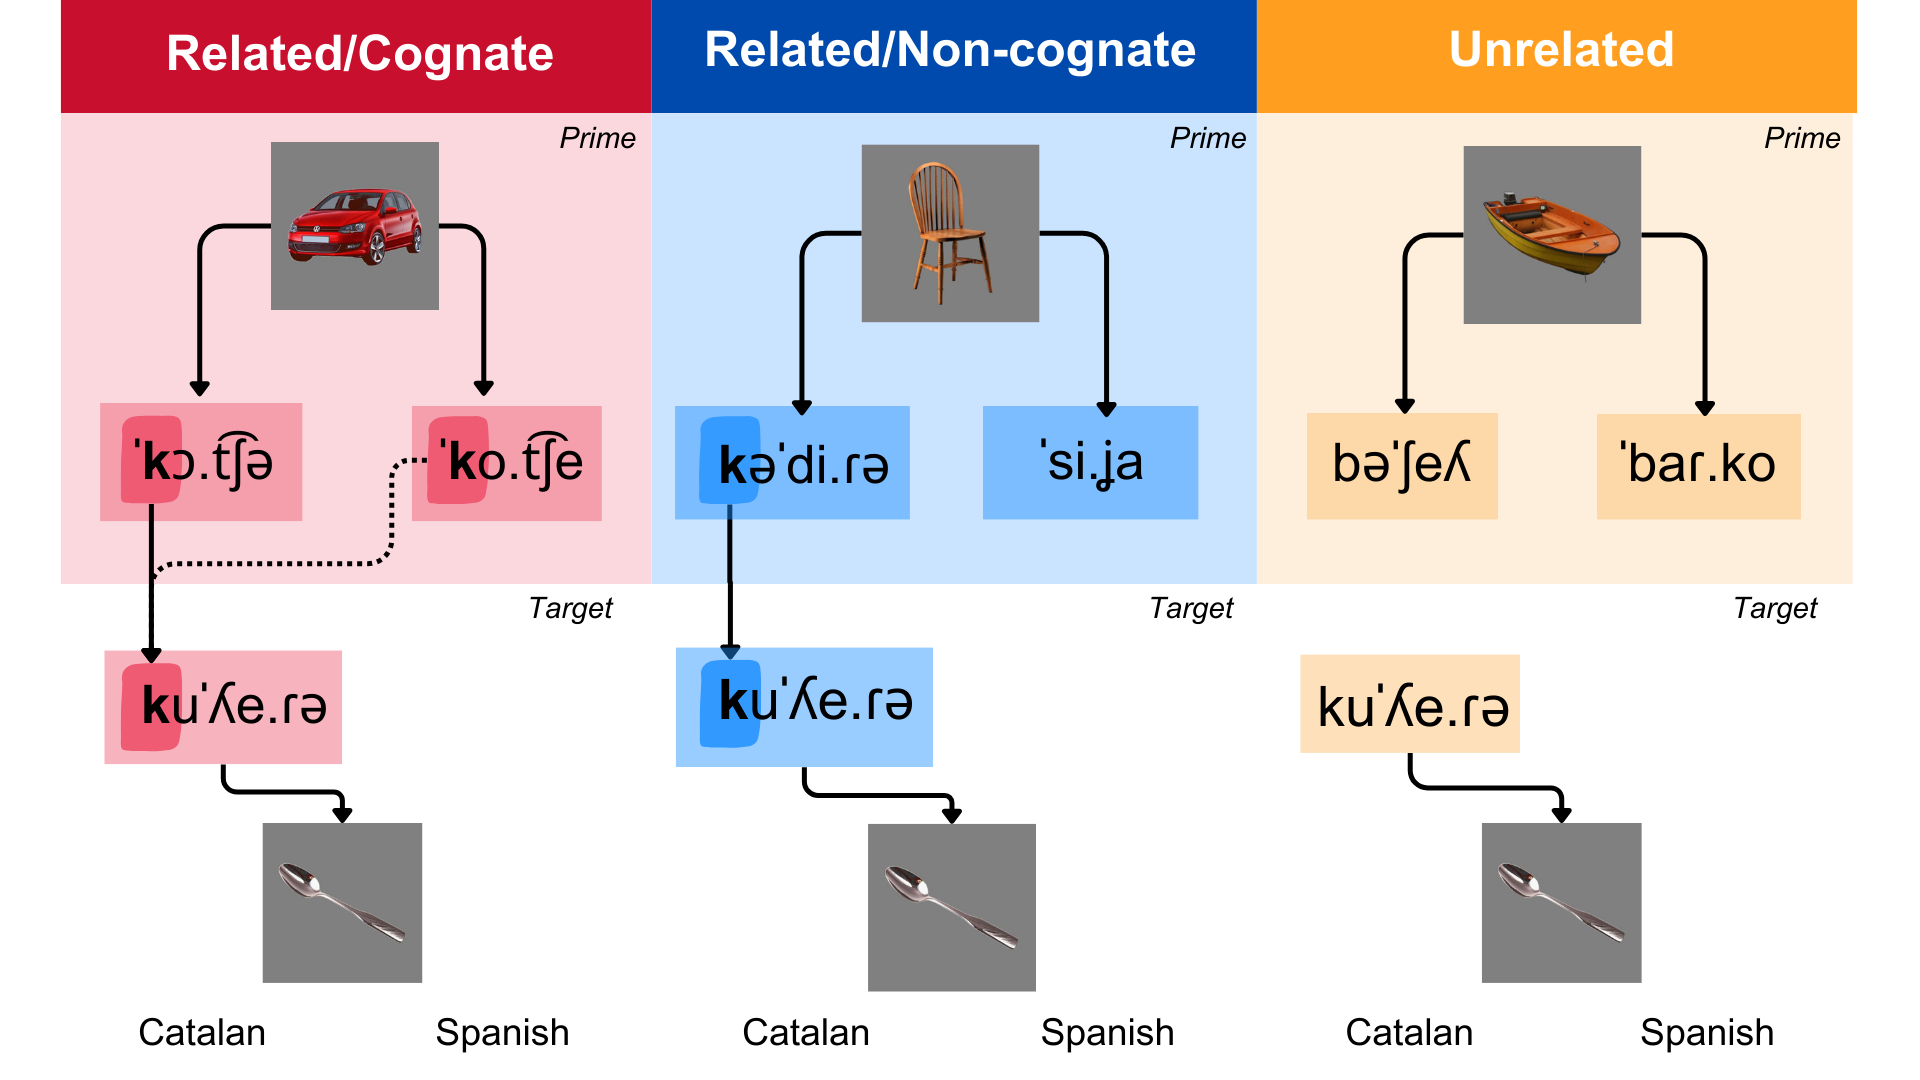
\includegraphics{chapters/../_assets/img/hypotheses.png}

}

\caption{\label{fig-hypotheses}Predicted priming effects (or their
absence) in the \emph{Related/Cognate}, \emph{Related/Non-cognate}, and
\emph{Unrelated} conditions, with examples for a participant tested in
Catalan. Words represent lexical representations. Lexical
representations of the task-relevant language (Catalan) are depicted
inside grey boxes. Solid arrows indicate within-language priming
effects, and dashed lines indicate cross-language priming effects. In
\emph{Related/Cognate} (A) and \emph{Related/Non-cognate} (B) trials,
the recognition of the Catalan target word \textipa{ku"Le.R@}
{[}spoon{]} is predicted to be modulated by the prior activation of the
prime label in Catalan. In \emph{Related/Cognate} trials, the parallel
activation of the prime label in Spanish is predicted to increase the
strength of the priming effect.}

\end{figure}

In line with previous studies in monolinguals, we further predicted that
the strength of the lexical interference effects in the
\emph{Related/Non-cognate} and \emph{Related/Cognate} conditions would
be associated to participants' vocabulary size. Target word recognition
should be delayed by the activation of a larger cohort of phonologically
related words (Avila-Varela et al., 2021; Chow, Davies, et al., 2017;
Mani \& Plunkett, 2011a; Mayor \& Plunkett, 2014). We defined vocabulary
size as the amount of words participants were reported to understand in
their dominant language by their caregivers. The choice of the dominant
language for calculating vocabulary sizes is due to several reasons.
First, it allows a more fair comparison between monolinguals (who do not
know any language other than their dominant language) and bilinguals
(who may know words in a second language). Second, since participants
were tested exclusively in their dominant language, their vocabulary
size in the dominant language is more likely to be associated to
participants' performance in the task. Third, previous work on word
recognition in bilinguals suggests that vocabulary size in the dominant
language predicts participants' performance better than total vocabulary
(in which vocabulary sizes in both languages are summed together)
(Marchman et al., 2010).

Because of the short-lived effects of cross-language activation on
lexical processing, and to maximise the probability of detecting priming
effects, we introduced a change in the sequence of the trials relative
to the original implementation by Mani \& Plunkett (2010). We presented
target auditory labels immediately after the offset of the prime
picture, and before the onset of the target and distractor pictures. By
presenting prime pictures and target auditory labels closer in time,
implicit naming of the prime picture should be more likely to influence
the recognition of the target word. To test the effects of this
methodological change, we first run a control experiment, Study 1, in
which we tested a group of same-aged English monolinguals. In Study 2,
we tested a group of monolinguals and bilinguals learning Catalan and
Spanish.

\hypertarget{study-1}{%
\section{Study 1}\label{study-1}}

In this study, we conducted a conceptual replication of Mani \& Plunkett
(2010) and Mani \& Plunkett (2011a). We tested a group of English
monolinguals aged 20 to 32 months, living in the Oxfordshire area
(United Kingdom). As just said, participants were tested exclusively in
English. As in the original studies, we manipulated the phonological
relationship between the prime and the target label. We expected
participants' target looking to change as a function of the phonological
relatedness between the prime and target English labels. This would
reveal that participants implicitly named the prime pictures, generating
a phonological label that influenced the subsequent recognition of a
phonologically related word. In half of the trials the English prime
label was phonologically related to its Spanish translation, that it
they were cognates; in the other half they were not phonologically
related (non-cognates)\footnote{It was initially planned to collected
  data from English monolinguals and English-Spanish bilinguals in
  Oxford, therefore the manipulation of the cognate status of the words
  in English and Spanish. Due to time limitations imposed by the COVD-19
  lockdown between 2020 and 2022, collecting data from bilinguals was
  not possible. We report the available data from English monolinguals
  as a control for Catalan and Spanish monolinguals and bilinguals from
  Barcelona in Study 2.}. Given participants' lack of knowledge of
Spanish (or any language other than English), participants' performance
was predicted to be unaffected by the cognate status of the primes.

In this study, we conducted a conceptual replication of Mani \& Plunkett
(2010) and Mani \& Plunkett (2011a). We tested a group of English
monolinguals aged 20 to 32 months, living in the Oxfordshire area
(United Kingdom). As highlighted in the introduction, participants were
tested exclusively in English, their dominant language. As in the
original studies, we manipulated the phonological relationship between
the prime and the target label. In line with Mani \& Plunkett (2011a),
we predicted participants' target looking to change as a function of the
phonological relatedness between the prime and target English labels.
This would reveal that participants implicitly named the prime pictures,
generating a phonological label that influenced the subsequent
recognition of a phonologically related word. To establish a monolingual
baseline for all conditions in Study 2, we also manipulated the cognate
status of the prime in English and Spanish: in half of the trials the
English prime label was phonologically related to its Spanish
translation. Given participants' lack of familiarity with Spanish (or
any language other than English), participants' performance was
predicted to be unaffected by the cognate status of the primes.

\hypertarget{methods}{%
\subsection{Methods}\label{methods}}

All materials, data, and reproducible code can be found at the OSF
(\href{https://osf.io/ckydb/}{https://osf.io/hy984/}) and GitHub
(\url{https://github.com/gongcastro/cognate-priming}) repositories. This
study was conducted according to guidelines laid down in the Declaration
of Helsinki, and was approved by the Drug Research Ethical Committee
(CEIm) of the IMIM Parc de Salut Mar, reference 2020/9080/I and the
Medical Sciences Research Ethics Board at the University of Oxford,
reference R60939/RE009. Before every testing session, caregivers were
asked to read and sign an informed consent form, and were given a token
of appreciation at the end of it.

\hypertarget{participants}{%
\subsubsection{Participants}\label{participants}}

We collected data from 112 children (41 female, 68 male, with three
additional participants' sex not being reported; Age: \emph{Mean} =
26.36 months, \emph{SD} = 4.01, \emph{Range} = 20.03--32.5) (see
Table~\ref{tbl-participants} for a detailed summary of participants' age
and language profile), living in the Oxfordshire area (United Kingdom).
Participants were tested at the Oxford BabyLab at the University of
Oxford. Families were recruited from maternity rooms in private
hospitals and social media, and contacted via phone when the child's age
spanned between 20 and 32 months. From the 112 children that
participated, 97 participated once, and 15 participated twice. Recurrent
participants were tested with at least 2.82 months of difference. We
gathered a total of 127 testing sessions. All participants were being
raised in exclusively British English monolingual homes. Participants'
vision was normal, none used glasses or any other type of vision
corrector.

\newpage

\blandscape

\hypertarget{tbl-participants}{}
\begin{table}
\caption{\label{tbl-participants}Demographic and linguistic profile of testing sessions in Study 1. The
number of excluded testing sessions and participants is indicated
between parentheses. }\tabularnewline

\centering
\begin{tabular}{lrrrrrl}
\toprule
\multicolumn{4}{c}{ } & \multicolumn{3}{c}{Degree of Exposure (\%)} \\
\cmidrule(l{3pt}r{3pt}){5-7}
\multicolumn{1}{c}{ } & \multicolumn{2}{c}{Sample size} & \multicolumn{1}{c}{Age (months)} & \multicolumn{1}{c}{English} & \multicolumn{1}{c}{Catalan} & \multicolumn{1}{c}{Spanish} \\
\cmidrule(l{3pt}r{3pt}){2-3} \cmidrule(l{3pt}r{3pt}){4-4} \cmidrule(l{3pt}r{3pt}){5-5} \cmidrule(l{3pt}r{3pt}){6-6} \cmidrule(l{3pt}r{3pt}){7-7}
  & Test sessions & Participants & \textit{M} (\textit{SD}) & \textit{M} (\textit{SD}) & \textit{M} (\textit{SD}) & \textit{M} (\textit{SD})\\
\midrule
\addlinespace[0.3em]
\multicolumn{7}{l}{\textbf{Study 1: Monolingual}}\\
\hspace{1em}English dominant & 89 (21) & 79 (21) & 26.47 (4.05) & 100.00 (0.00) & 0.00 (0.00) & 0.00 (0.00)\\
\midrule
\addlinespace[0.3em]
\multicolumn{7}{l}{\textbf{Study 2: Monolingual}}\\
\hspace{1em}Catalan dominant & 65 (7) & 46 (6) & 25.19 (3.81) & 0.18 (0.79) & 61.98 (10.31) & 37.65 (10.47)\\
\hspace{1em}Spanish dominant & 42 (7) & 31 (7) & 25.58 (3.41) & 0.38 (1.56) & 38.55 (10.42) & 61.12 (11.00)\\
\midrule
\addlinespace[0.3em]
\multicolumn{7}{l}{\textbf{Study 2: Bilingual}}\\
\hspace{1em}Catalan dominant & 87 (8) & 50 (7) & 25.78 (3.91) & 0.37 (2.20) & 95.11 (6.17) & 4.54 (5.98)\\
\hspace{1em}Spanish dominant & 46 (7) & 28 (6) & 25.18 (3.80) & 0.24 (0.85) & 8.74 (6.40) & 90.80 (6.38)\\
\bottomrule
\end{tabular}
\end{table}

\elandscape

We collected vocabulary data using parental responses to the Oxford
Communicative Development Inventory (OCDI) (Hamilton et al., 2000). The
OCDI is an adaptation of the MacArthur-Bates Communicative Development
Inventory (Fenson et al., 1994) to British English. The OCDI includes a
vocabulary checklist containing 418 words from 21 semantic-functional
categories (e.g., action words, animals, household objects, adverbs,
etc.). For each word, caregivers are asked to answer if they child is
able to \emph{understand}, \emph{understand and say} or does not
understand or say the word. We calculated participants' receptive
vocabulary size scores as the number of words that caregivers marked as
\emph{understands} or \emph{understands and says}. Families were sent
the questionnaire immediately after each experimental session, and were
given two weeks to fill it. In the case that a complete response to the
OCDI was not provided within the two-week limit, the participants'
testing session was excluded from the analyses (\emph{n} = 3).
Figure~\ref{fig-vocabulary-oxf} shows the distribution of participants'
vocabulary sizes across ages.

\begin{figure}

{\centering 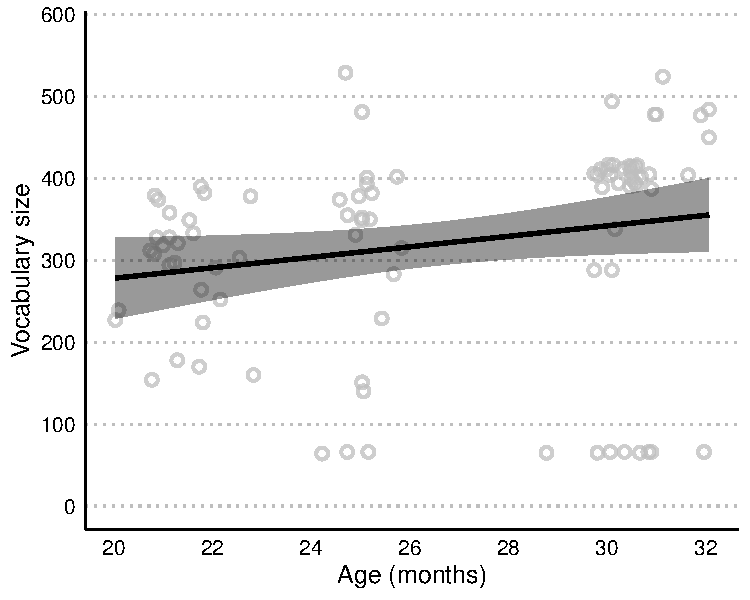
\includegraphics[width=0.7\textwidth,height=\textheight]{chapters/03-chapter-3_files/figure-pdf/fig-vocabulary-oxf-1.pdf}

}

\caption{\label{fig-vocabulary-oxf}Participant receptive vocabulary
sizes across ages and language profiles. For descritive purposes, mean
and standard error of the mean are indicated, as calculated using a
linear regression model.}

\end{figure}

\hypertarget{design}{%
\subsubsection{Design}\label{design}}

Participants were presented with 32 trials in random order, which
belonged to two conditions: \emph{Related} and \emph{Unrelated} trials.
In \emph{Related} trials (\emph{n} = 16), the English label of the prime
was phonologically related to the target label, sharing phonological
onset (e.g.,
/\textbf{\textipa{"t}}\textipa{\*ri:}/\(_{\text{ENG}} [\text{tree}]\)--/\textbf{\textipa{"t}}\textipa{\*r2k}/\(_{\text{ENG}} [\text{truck}]\)).
In \emph{Unrelated} trials, the prime and target labels did not share
phonological onset (e.g.,
/\textipa{"dO:}/\(_{\text{ENG}} [\text{door}]\)--/\textipa{"s6k}/\(_{\text{ENG}} [\text{sock}]\)).
Especial attention was paid to avoiding semantic or taxonomic
relationships between prime and target words, and between prime and
distractor words. Distractors were always phonologically unrelated to
the prime and target labels in the same trial.

Figure~\ref{fig-task} illustrates the sequence of a trial. Each trial
started with the presentation of an attention getter for 3,000 ms. Then,
the prime picture was presented in silence in the centre of the screen
for 1,500 milliseconds. Fifty milliseconds after the offset of the prime
image, an auditory label was played, 700 milliseconds after the onset of
the word, the target and distractor pictures were presented side-by-side
during 1,000 milliseconds until the end of the trial. After this, the
attention getter of the next trial was immediately presented. Each
experimental session lasted approximately 10 minutes.

\newpage

\blandscape

\begin{figure}

{\centering 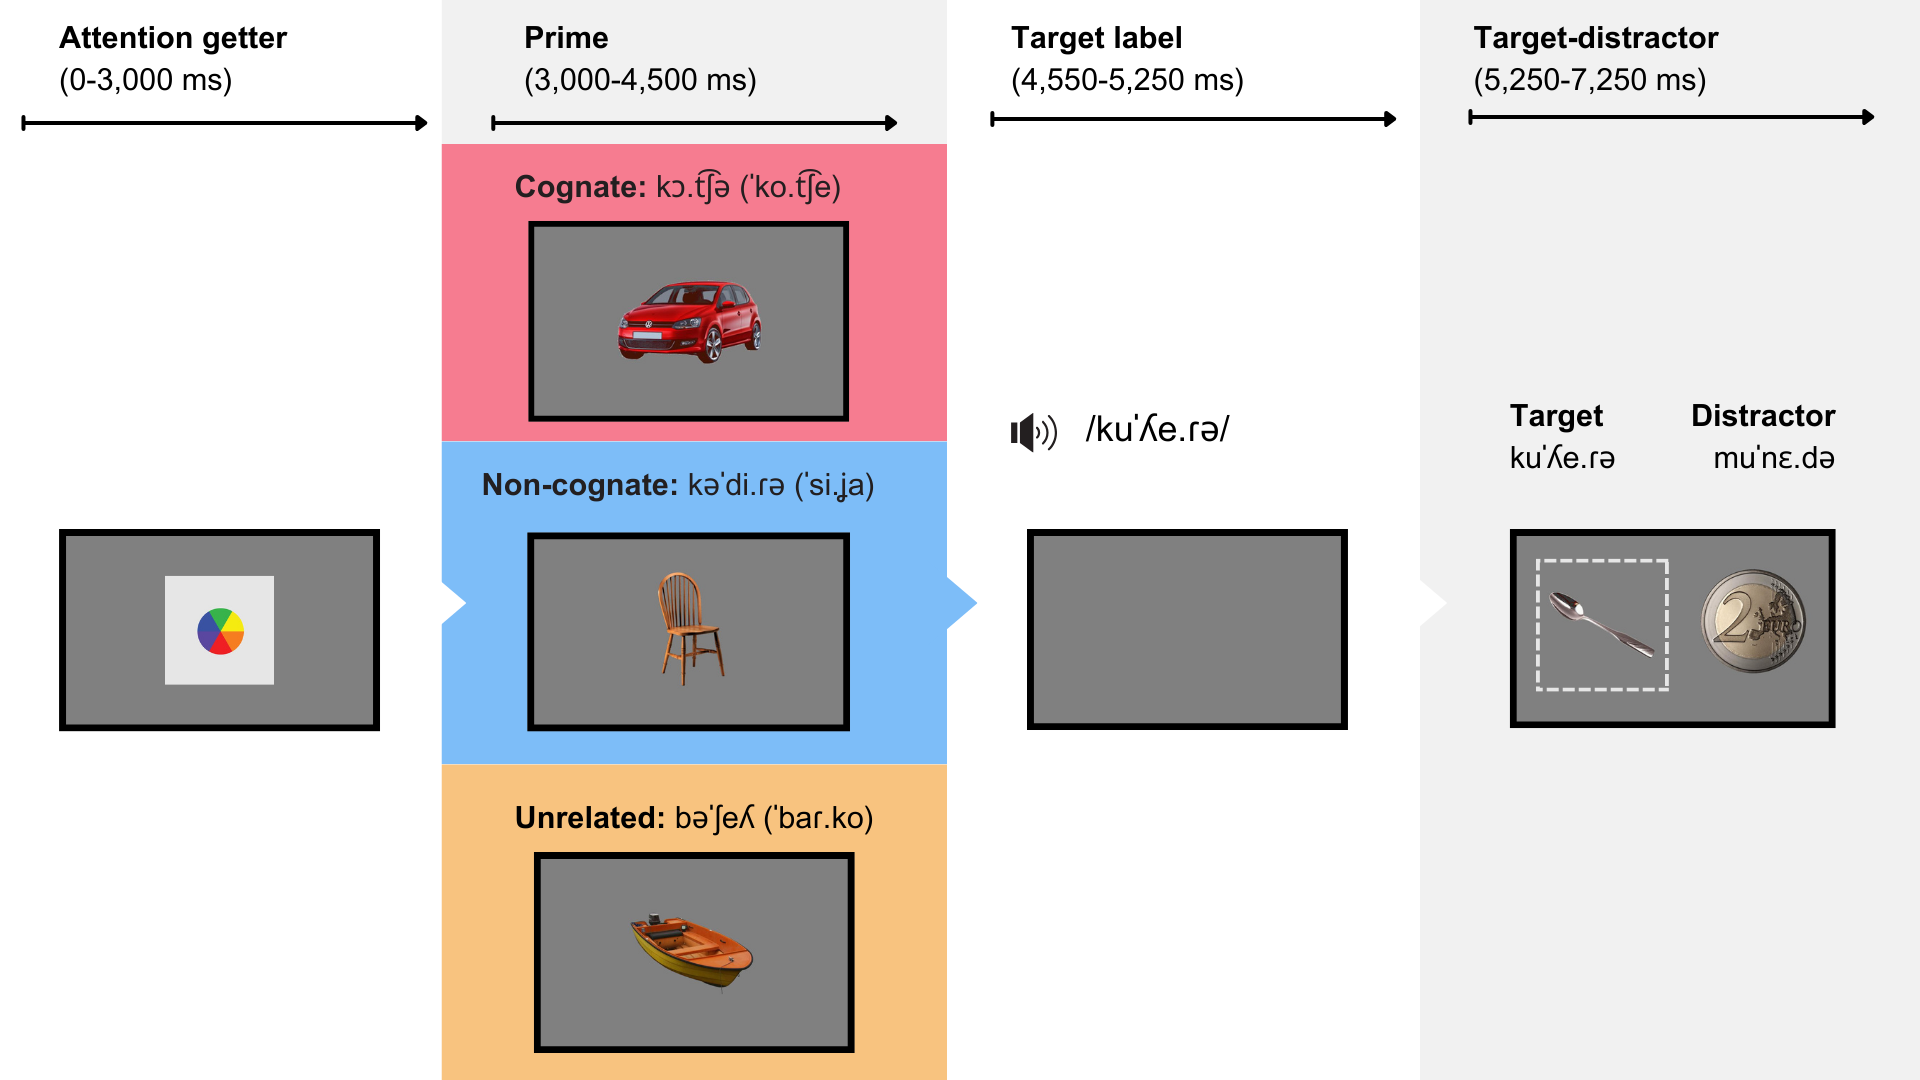
\includegraphics{chapters/../_assets/img/design.png}

}

\caption{\label{fig-task}Experimental task design with examples in
Catalan. In each trial, the prime image is presented in silence for
1,500 ms. Then the auditory target label is presented, and finally the
target and distractor pictures are presented side-by-side for 2,000 ms.
In cognate trials (\emph{n} = 8), Catalan \emph{and} Spanish prime
labels shared phonological onset with the target label. In non-cognate
trials (\emph{n} = 8), only the Catalan prime label shared phonological
onset with the target label. In unrelated trials (\emph{n} = 16), none
of the prime labels shared phonological onset with the target label.}

\end{figure}

\elandscape

\hypertarget{stimuli}{%
\subsubsection{Stimuli}\label{stimuli}}

We created four lists of trials, across which the same target-distractor
pair appeared with a different prime, counterbalancing the condition to
which it belonged. For instance, in list one the
\emph{ball}-\emph{trousers} pair was preceded by \emph{bike}
(\emph{Related/Cognate}), by \emph{butterfly}
(\emph{Related/Non-cognate}) in list two, and by \emph{star} and
\emph{nose} (\emph{Unrelated}) in lists three and four (see Appendix A
for a detailed description of the stimuli). Table~\ref{tbl-stimuli}
shows a detailed summary of the stimuli properties, broken down by trial
type and testing language. Trials included in each condition had
equivalent length (number of phonemes) and lexical frequency. Lexical
frequencies were extracted from the English corpora from the CHILDES
database (MacWhinney, 2000; Sanchez et al., 2019b) as counts per million
words, and transformed into Zipf scores for easier cross-language
comparison (Van Heuven et al., 2014b; Zipf, 1945). Audios had an average
duration of 864.23 ms (\emph{SD} = 148.53, \emph{Range} = 570--1,250).

\newpage

\blandscape

\hypertarget{tbl-stimuli}{}
\begin{table}
\caption{\label{tbl-stimuli}Summary of stimuli properties in Studies 1 and 2 by trial type. Values
are summarised using the mean and the standard deviation (between
parentheses). }\tabularnewline

\centering
\begin{tabular}{lrrrrrr}
\toprule
\multicolumn{1}{c}{ } & \multicolumn{2}{c}{Word length (phonemes)} & \multicolumn{2}{c}{Lexical frequency (Zipf)} & \multicolumn{2}{c}{Familiarity (\%)} \\
\cmidrule(l{3pt}r{3pt}){2-3} \cmidrule(l{3pt}r{3pt}){4-5} \cmidrule(l{3pt}r{3pt}){6-7}
Condition & \textit{M} (\textit{SD}) & \textit{M} (\textit{SD}) & \textit{M} (\textit{SD}) & \textit{M} (\textit{SD}) & \textit{M} (\textit{SD}) & \textit{M} (\textit{SD})\\
\midrule
\addlinespace[0.3em]
\multicolumn{7}{l}{\textbf{Study 1: English}}\\
\hspace{1em}Related/Cognate & 5.00 (1.24) & 4.50 (1.34) & 4.63 (0.53) & 4.75 (0.39) & 0.62 (0.10) & 0.70 (0.15)\\
\hspace{1em}Related/Non-cognate & 5.75 (2.72) & 4.50 (1.34) & 4.75 (0.18) & 4.75 (0.39) & 0.61 (0.13) & 0.71 (0.15)\\
\hspace{1em}Unrelated & 5.24 (2.27) & 4.33 (1.47) & 4.68 (0.38) & 4.73 (0.38) & 0.67 (0.18) & 0.73 (0.17)\\
\midrule
\addlinespace[0.3em]
\multicolumn{7}{l}{\textbf{Study 2: Catalan}}\\
\hspace{1em}Related/Cognate & 4.50 (1.34) & 4.88 (1.28) & 5.07 (0.33) & 4.83 (0.26) & 0.85 (0.09) & 0.69 (0.23)\\
\hspace{1em}Related/Non-cognate & 4.88 (1.47) & 5.17 (1.33) & 5.01 (0.37) & 4.76 (0.25) & 0.83 (0.11) & 0.70 (0.22)\\
\hspace{1em}Unrelated & 5.00 (1.51) & 4.98 (1.31) & 4.91 (0.31) & 4.89 (0.25) & 0.76 (0.15) & 0.68 (0.22)\\
\midrule
\addlinespace[0.3em]
\multicolumn{7}{l}{\textbf{Study 2: Spanish}}\\
\hspace{1em}Related/Cognate & 4.50 (0.88) & 6.12 (1.55) & 5.10 (0.31) & 4.77 (0.29) & 0.65 (0.24) & 0.47 (0.24)\\
\hspace{1em}Related/Non-cognate & 5.25 (1.21) & 5.92 (1.54) & 4.94 (0.42) & 4.71 (0.26) & 0.68 (0.21) & 0.50 (0.26)\\
\hspace{1em}Unrelated & 4.62 (1.06) & 5.73 (1.53) & 4.94 (0.28) & 4.69 (0.23) & 0.64 (0.23) & 0.46 (0.27)\\
\bottomrule
\end{tabular}
\end{table}

\elandscape

The auditory stimuli were natural exemplars of the selected target
words, spoken by a Southern British English female speaker who was
instructed to pronounce each word in a toddler-directed manner. We used
the Audacity and Praat (Boersma \& Van Heuven, 2001) software packages
to trim, denoised, and normalised their amplitude. The visual stimuli
were realistic photographic representations of a typical exemplars of
the prime, target, and distractor words. Image backgrounds were removed
from the original pictures using the GNU Image Manipulation Program
(GIMP), resized to a rectangle of a maximum of 400 pixels height or
wide, and finally placed in the centre of a 50\% grey rectangle square
of 500 \(\times\) 500 pixels. The final stimuli had a resolution of 72
dpi. When presented in the eye-tracker screen, the areas of interest
(AOI) occupied an area of 13.23 \(\times\) 13.23 cm (11.613\(^{\circ}\)
visual angle from participants' perspective).

\hypertarget{procedure}{%
\subsubsection{Procedure}\label{procedure}}

Testing took place in a sound-proof room at the BabyLab of the
University of Oxford. Participants sat on their caregivers' lap in a
dimly lit testing booth while the experimenter conducted the experiment
from outside. Caregivers were instructed to keep their eyes shut (to
avoid recording their gaze, instead of the participant's), to be still,
and to avoid interacting with the participant verbally or non-verbally.
Participants sat at approximately 65 cm from the eye-tracker and a
23-inches screen with \(1929\times1080\) resolution. The study was run
on Windows 7 (64-bit), using a custom Matlab script, PresentMate, based
on the PsychToolbox-3 extension (3.0.10, 32 bit) (Brainard \& Vision,
1997; Kleiner et al., 2007; Pelli \& Vision, 1997). Visual fixations
were recorded using a Tobii TX300 eye-tracker (Tobii Technology,
Stockholm, Sweden) and a 23-in screen of 1920 \(\times\) 1080
resolution. The Tobii Analytics SDK 3.0 was used to interact with the
eye-tracking while the experiment was running. Sampling rate was set at
120 Hz. A 9-point calibration was performed before every experimental
session, in which the picture of a colourful beach ball was presented.
We set a 55\% grey background for the screen during calibration and
stimuli presentation. Auditory stimuli were presented through two
loudspeakers located behind the screen, one to each side. The
experimenter monitored the experimental from outside the room using a
centrally located video camera place above the screen. After a
successful calibration the experimenter triggered the onset of the first
trial. Trials were presented uninterruptedly and without intervention of
the experimenter until the 32 trials were presented, or the experimental
session had to be stopped because of the participant's behaviour.

\hypertarget{data-analysis}{%
\subsubsection{Data analysis}\label{data-analysis}}

\textbf{Data processing}. We defined a time window of interest from 200
ms after target and distractor pictures onset until the end of the trial
at 2,000 ms when both pictures disappeared from screen. The first 200 ms
of the test phase were discarded to avoid modelling fixations driven by
processes other than auditory word recognition (Fernald et al., 1998,
2001). Missing eye-tracker samples were interpolated using the
last-observation-carried-forward (see Zettersten et al., 2022 for a
similar approach), with a maximum of 20 maximum consecutive missing
samples being interpolated (an equivalent of 166.67). Target looking
probability was calculated as the empirical logit, using the number of
samples inside the time bin in which the participant was looking at the
target and distractor AOI (see Equation~\ref{eq-elogit}) (Agresti, 2012;
Barr, 2008), as follows:

\begin{equation}\protect\hypertarget{eq-elogit}{}{
\eta' = \ln\bigg(\frac{\text{Target} + 0.5}{ \text{Distractor} + 0.5}\bigg)
}\label{eq-elogit}\end{equation}

We gathered data from 3,484 trials from 110 testing sessions, generated
from 97 distinct participants. We excluded trials in which participants
failed to provide 50\% valid eye-tracking samples (equivalent to 750 ms)
during the prime phase (\emph{n} = 829) or 50\% valid samples
(equivalent to 1,000 ms) during the target-distractor phase (\emph{n} =
650). We also excluded trials in which participants did not provide at
least 5\% of valid samples (equivalent to 100 ms) of target or
distractor looking in the test phase (\emph{n} = 1,003) (see Floccia et
al., 2020; Mani et al., 2012 for a similar approach).

After trials that matched any of the aforementioned exclusion criteria
from the data set, we excluded participants who did not provide at least
two valid trials in each condition (\emph{n} = 19), and participants
with a vocabulary size lower than 42, which corresponds to 10\% of the
words in the OCDI vocabulary checklist (\emph{n} = 3). The final data
set included 1,861 trials from 78 testing sessions, generated by 79
distinct participants. Of those participants, 69 provided data from one
experimental session, 10 provided data from two experimental sessions,
and NA provided data from three experimental sessions. From the trials
included in the final data set, 915 were \emph{Unrelated} trials (502
previously excluded), and 946 were \emph{Related} trials(470 previously
excluded).

\textbf{Modelling approach}. We used Bayesian Hierarchical General
Additive Models (HGAMs) to model the data (Pedersen et al., 2019), using
a Gaussian distribution to model the the logit of target looking. First,
we fit a model (\(\mathcal{M}_0\)) that included the main effects of
\emph{Condition} and \emph{Age} as fixed effects in the model. We set an
\emph{a priori} contrast for the \emph{Condition} predictor (Schad et
al., 2020), comparing \emph{Unrelated} and \emph{Related} trials
(sum-coded as \texttt{-0.5} and \texttt{+0.5}. Before entering the
model, the \emph{Age} predictor was standardised by subtracting from
each observation the mean of the predictor, and dividing the result from
the standard deviation of the predictor. We included the variable
\emph{Session}---which indexes individual testing sessions that may
belong to the same participant---as grouping variable, nested within the
\emph{Participant} grouping variable---which indexes a distinct
participant. This nested random effects structure incorporates the
longitudinal design of data collection, in which multiple participants
were tested more than once at different ages. We added by-session
intercepts and \emph{Condition} slopes, and by-participant intercepts
and \emph{Age} slopes. To model the time course of target looking across
time bins, we included B-splines for the main effect of \emph{Time}, and
for the \emph{Condition} predictor (Wood, 2017). For both splines, we
specified \(k = 8\) basis functions or \emph{knots}.
Equation~\ref{eq-model} shows a formal implementation of the model.

We implemented this model using \texttt{brms} (Bürkner, 2017), an R
interface to the Stan probabilistic language (2.33.0) (Carpenter et al.,
2017). We ran two iteration chains using the by-default No U-Turn
Sampler algorithm with 1,000 iterations each and an additional 1,000
warm-up iterations per chain.

\newpage

\begin{equation}\protect\hypertarget{eq-model}{}{
\begin{aligned}
&\textbf{Target looking by participant } i \textbf{ in session } j \\
y_{ij} &\sim \mathcal{N}(\mu_{ij}, \sigma_{ij}) \\\\
&\textbf{Distributional parameters:} \\
\eta'(\mu_{ij}) &= (\beta_0 + u _{0_{ij}}) +
(\beta_1 + u _{1_{ij}}) \text{Condition} + \beta_{2} \text{Age} + \sum_{w = 1}^k b_{w} \beta_{3_{k}} \text{Time} + \\
\text{where:} \\
&\eta'\text{ is the empirical logit of target fixations} \\
&b_{w} \text{ is the cubic spline of the } w \text{ basis function} \\
&k \text{ is the number of knots in the spline }(k = 8) \\
&\textbf{Prior:} \\
\beta_{0-3} &\sim \mathcal{N}(0, 0.5) \\
u_{0-1_{ij}} &\sim \mathcal{N}(0, \sigma_{0-2})\\
b_{w} &\sim \text{MVN}(0, \tau) \\
\sigma_{0-1}, \tau &\sim \text{Exponential}(6)\\
\rho_{0-1} &\sim LKJCorr(6)\\
\text{where:}\\
&\rho_{0-1} \text{ are the correlation parameters for } \sigma_{0-2}
\end{aligned}
}\label{eq-model}\end{equation}

\hypertarget{results}{%
\subsection{Results}\label{results}}

\hypertarget{priming-effects}{%
\subsubsection{Priming effects}\label{priming-effects}}

We tested the differences between the conditions of interest in two
ways. First, we examined the posterior distribution of the regression
coefficients of the linear predictors in model \(\mathcal{M}_0\) (see
Equation~\ref{eq-model}). We assessed the practical relevance of the
coefficients following J. K. Kruschke \& Liddell (2018). We specified a
region of practical equivalence (ROPE) from -0.1 to +0.1, in the logit
scale. This region indicates the range of values that we considered
equivalent to zero. We then summarised the posterior distribution of
each regression coefficient with the 95\% highest density interval
(HDI). This interval contains the true value of this coefficient with
95\% probability, given the data. Finally, we calculated the proportion
of posterior samples in the 95\% HDI that fell into the ROPE, noted as
\(p(\text{ROPE})\), which indicates the probability that the true value
of the regression coefficient falls into the ROPE (and therefore should
be considered equivalent to zero). For example, \(p(\text{ROPE})=.80\)
indicates that, given our data, there is a 80\% probability that the
true value of the coefficient falls within the ROPE, and can therefore
be considered equivalent to zero.

Overall, the average participant' target looking time exceeded chance
levels, as indicated by the fact that the 95\% HDI of the intercept term
excluded zero (\(\beta\) = 0.381, 95\% HDI = {[}0.292, 0.464{]}) and all
of its posterior samples fell outside of the ROPE. The 95\% HDI of the
coefficient of \emph{Age} had a positive sign, but did not exclude zero
(\(\beta\) = -0.023, 95\% HDI = {[}-0.110, 0.058{]}), and overlapped
completely with the ROPE, indicating that participants from all ages
showed equivalent overall target word recognition. The 95\% HDI of the
contrast of the \emph{Condition} predictor---comparing \emph{Unrelated}
and \emph{Related} trials---included zero (\(\beta\) = 0.093, 95\% HDI =
{[}-0.035, 0.235{]}), and 50.07\% of its posterior samples fell within
the ROPE.

Second, we examined the differences between the priming conditions in
the time course of the trial, incorporating the smooth functions of the
HGAMs to generate marginal posterior predictions for each condition
across for each time point. Figure~\ref{fig-epreds-oxf} shows the
posterior predictions of the model for each condition, and a summary of
the difference between the \emph{Unrelated} and \emph{Related}
conditions, at each time point to test the practical relevance of these
differences, were compared their 95\% HDI against the {[}-0.1, +0.1{]}
ROPE. This analysis revealed a similar pattern of results to the
previously shown: predicted target looking for the three conditions
overlaps across the full time course of the trial.

\begin{figure}

{\centering 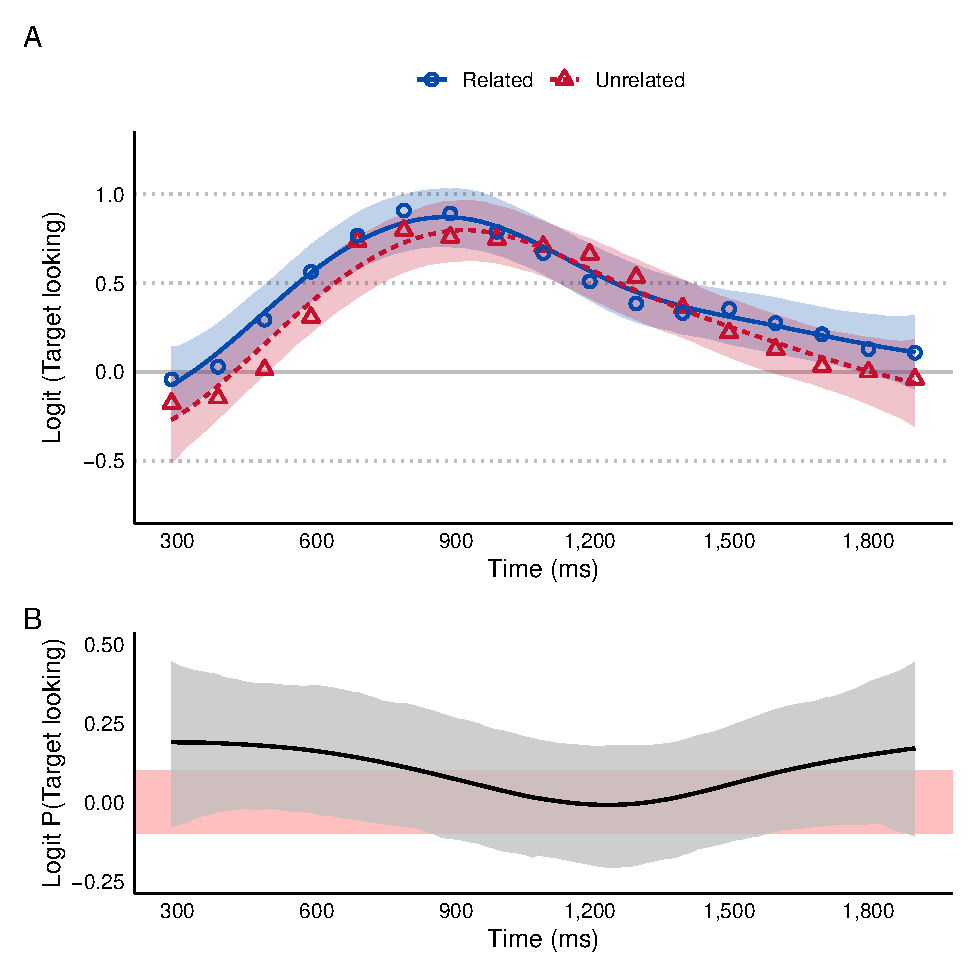
\includegraphics{chapters/03-chapter-3_files/figure-pdf/fig-epreds-oxf-1.pdf}

}

\caption{\label{fig-epreds-oxf}Time course of target fixations in Study
1. A) Posterior mean predictions of the time course of target fixation
in the test phase. B) Posterior mean prediction of the time course of
the differences in target looking time between conditions. Intervals
represent the 95\% CrI of the posterior predictions. Lines indicate the
mean of the posterior predictions.}

\end{figure}

\hypertarget{age-and-vocabulary-size-effects}{%
\subsubsection{Age and vocabulary size
effects}\label{age-and-vocabulary-size-effects}}

To test our hypotheses regarding the role of age and vocabulary size on
the emergence of priming effects, we compared the fit of model
\(\mathcal{M}_0\) against the fit of other models including the two-way
interaction between \emph{Condition} and \emph{Age} (\(\mathcal{M}_1\)),
or the two-way interaction between \emph{Condition} and
\emph{Vocabulary} (\(\mathcal{M}_2\)), and all main effects involved. As
with \emph{Age}, the \emph{Vocabulary} predictor was standardised before
entering the model. We compared the models using one-out
cross-validation (LOO-CV) as a benchmark of model performance, using a
Pareto-smoothed importance sampling (PSIS) approximation (Vehtari et
al., 2017). A better performance by models \(\mathcal{M}_1\) or
\(\mathcal{M}_2\) over \(\mathcal{M}_0\) would point to \emph{Age} or
\emph{Vocabulary}, respectively, playing a substantial role in
participants' word-recognition, or on the emergence of priming effects.
Table~\ref{tbl-loos-oxf} shows a summary of the predictive performance
of the models, as quantified by the expected log-predictive density
(\emph{ELPD}), and its standard error (\emph{SE}, a measure of
uncertainty around the \emph{ELPD}). Overall, all models, performed
equivalently, as shown by the small difference in \emph{ELPD}, relative
to the uncertainty of the estimates. This suggests that participants'
target looking during the test phase can be predicted with relative
accuracy without taking into account the age or vocabulary size of the
participants.

\hypertarget{tbl-loos-oxf}{}
\begin{table}
\caption{\label{tbl-loos-oxf}Leave-one-out cross validation outcomes, comparing the predictive
performance of the models in Study 1. \(ELDP\): sum of expected log
pointwise predictive density for a new data set. \(ELDP_{SE}\): standard
error of the \(ELPD\), which indictes the uncertainty about the
predictive performance for unknown future data. \(\Delta\): pairwise
difference in \(ELPD\) for two models. The difference is computed
relative to the model with lowest \(ELPD\) (best fitting model).
\(\Delta_{SE}\): standard error of component-wise differences of
\emph{ELPD} between two models. }\tabularnewline

\centering
\begin{tabular}{lrrrrr}
\toprule
  & Predictors & $ELDP$ & $ELDP_{SE}$ & $\Delta$ & $\Delta_{SE}$\\
\midrule
$\mathcal{M}_1$ & $\text{Age} \times \text{Condition}$ & -8,469.02 & 73.01 & - & -\\
$\mathcal{M}_0$ & $\text{Age} + \text{Condition}$ & -8,469.15 & 73.02 & -0.13 & 1.11\\
$\mathcal{M}_2$ & $\text{Vocabulary} \times \text{Condition}$ & -8,469.37 & 73.09 & -0.35 & 1.58\\
\bottomrule
\end{tabular}
\end{table}

\hypertarget{discussion}{%
\subsection{Discussion}\label{discussion}}

We found strong evidence of successful word recognition across
participants of all ages, but we did not observe any evidence of
phonological priming. English monolingual participants from all ages
showed an equivalent pattern of target looking in both \emph{Related}
and \emph{Unrelated} trials. In conclusion, we failed to replicate the
original studies by Mani \& Plunkett (2010) and Mani \& Plunkett
(2011a). The absence of a phonological priming effect suggest that
either English monolinguals did not generate implicit labels for the
prime pictures presented in silence, or that, if generated, such labels
did not interact with the subsequent recognition of the target word.
Both explanations conflict with both Mani and Plunkett's studies, and
also with previous studies suggesting that infants 12-months and older
already generate internal labels when presented with pictures of
familiar objects (Duta et al., 2012; Styles et al., 2015).

Adding the predictors \emph{Age} or \emph{Vocabulary size} as predictors
in the model, in interaction with \emph{Condition} did not increase the
fit of the model. This points to neither variable having a substantial
influence in participants' target looking behaviour across conditions.
These results diverge from previous studies reporting an increment in
word recognition speed (Fernald et al., 1998; Marchman \& Fernald,
2008), and stronger phonological priming effects in children with larger
vocabulary sizes (Avila-Varela et al., 2021; Chow, Davies, et al., 2017;
Mani \& Plunkett, 2011a). Overall, this results suggest that our
modification of the implicit naming task resulted in the loss of the
originally reported effect.

\hypertarget{study-2}{%
\section{Study 2}\label{study-2}}

The original planning of the present investigation was to run Study 1
first and once the procedure had been validated to start Study 2.
However, right at the beginning of data collection, the outbreak of
COVID-19 pandemic took place. At this point it was decided to run both
experiments in parallel. Data collection at the Barcelona site proceeded
at a faster rate than at Oxford. It was not until data collection was
well advanced in Barcelona that the results of study 1 were available.
This is the reason why Study 2 was run with the same procedure as
Experiment 1.

\hypertarget{methods-1}{%
\subsection{Methods}\label{methods-1}}

\hypertarget{participants-1}{%
\subsubsection{Participants}\label{participants-1}}

We collected data from 162 children living in the Metropolitan Area of
Barcelona (Spain), tested at the Laboratori de Recerca en Infància at
the Universitat Pompeu Fabra. Families were recruited from maternity
rooms in private hospitals and social media, and contacted via phone
when the child's age spanned between 20 and 32 months. From the 162
children that participated, 81 participated once, 55 participated twice,
and 26 participated three times. Recurrent participants were tested with
at least 2.06 months of difference. We gathered a total of 269 testing
sessions. Participants were divided into monolinguals and bilinguals
based on their relative degree of exposure to Catalan and Spanish,
estimated using an adaptation of the Language Exposure Questionnaire
(LEQ, Bosch \& Sebastian-Galles, 2001). We categorised participants as
monolingual if exposed to more than 80\% or more of the time to their
dominant language, and as bilingual otherwise. Eighty of the
participants were categorised as monolinguals (34 female, 48 male) and
83 as Catalan/Spanish bilinguals (49 female, 34 male) (see
Table~\ref{tbl-participants} for a detailed summary of participants' age
and language profile). Participants' vision was normal, none used
glasses or any other type of vision corrector.

We collected vocabulary data using parental responses to the Barcelona
Vocabulary Questionnaire (BVQ, Garcia-Castro, Ávila-Varela, et al.,
2023a), an online vocabulary checklist developed to assess the
vocabulary size of Catalan-Spanish bilingual toddlers, and inspired in
several adaptations of the the Communicative Developmental Inventory
(CDI, Fenson et al., 1994). This questionnaire has four versions, each
including a different but overlapping subset of words, from a total pool
of 542 words from 26 functional-semantic categories. Each version
included a Catalan and a Spanish vocabulary checklist. Catalan
checklists contained between 343 and 349 words, and Spanish checklists
contained between 349 and 349 words (see the Methods section of Chapter
1 for a detailed description of the questionnaire). Participants were
randomly allocated to one of the four versions. Recurrent participants
were always allocated to the same version. Families received a link to
the BVQ immediately after each experimental session, and were given two
weeks to fill it. It is common for children living in the Metropolitan
area of Barcelona to be exposed to both Catalan and Spanish in some
degree, even monolinguals. For this reason, we collected Catalan
\emph{and} Spanish vocabulary data from all participants in Study 2, but
for consistency with Study 1, we calculated vocabulary sizes for
participants in Study 2 as the number of words that caregivers reported
their child to \emph{understand} or \emph{understand and say} only in
the dominant language of the child (i.e., the language of test).

One hundred thirty-six (51\%) families failed to provide a complete
response to the vocabulary checklist within the two-week time limit. We
imputed missing vocabulary size scores using single imputation, taking
the vocabulary size scores of a pool of 542 additional participants for
which a successful response for the questionnaire had been gathered. We
used participants' age in months and their language profile (monolingual
or bilingual) as predictors. We used the \texttt{mice} R package (Van
Buuren \& Groothuis-Oudshoorn, 2011) to perform imputation using the
Bayesian linear regression method (see Appendix B).

\begin{figure}

{\centering 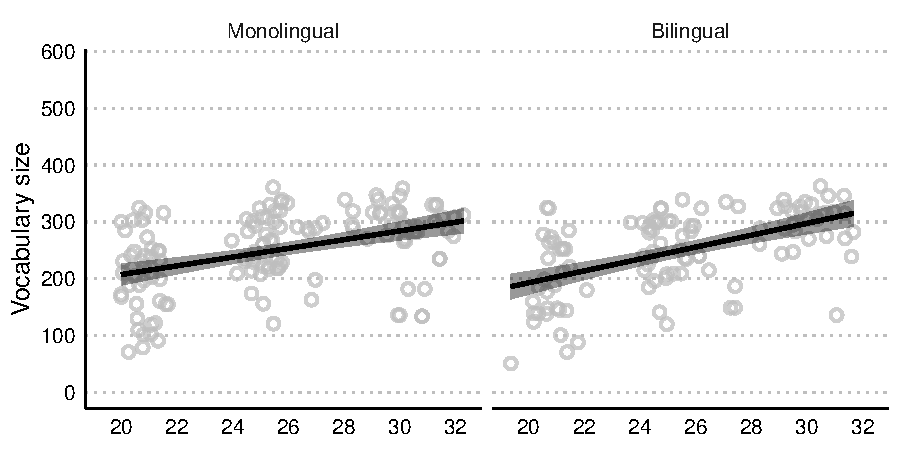
\includegraphics{chapters/03-chapter-3_files/figure-pdf/fig-vocabulary-bcn-1.pdf}

}

\caption{\label{fig-vocabulary-bcn}Participant receptive vocabulary
sizes across ages and language profiles in Study 2. For descritive
purposes, mean and standard error of the mean are indicated, as
calculated using a linear regression model.}

\end{figure}

\hypertarget{design-1}{%
\subsubsection{Design}\label{design-1}}

Participants were presented with 32 trials in random order, which
belonged to three conditions: \emph{Unrelated} trials (\emph{n} = 16),
\emph{Related/Non-cognate} (\emph{n} = 8), and \emph{Related/Cognate}
(\emph{n} = 8). In \emph{Unrelated} trials, the target label shared
phonological onset with the Catalan and Spanish labels of the prime
picture (e.g., prime:
/\textipa{"gos}/\(_{\text{CAT}}\)--/\textipa{"pe.ro}/\(_{\text{SPA}} [\text{dog}]\),
target: /\textipa{"ka.za}/\(_{\text{CAT}} [\text{house}]\), for a child
tested in Catalan). In \emph{Related/Non-cognate} trials, the target
shared phonological onset with the prime label in the test language, but
not with the prime label in the other language (e.g., prime:
/\textbf{\textipa{m}}\textipa{i"}\textdyoghlig\textipa{o}/\(_{\text{CAT}}\)
(/\textipa{kal.Te"in}/ \(_{\text{SPA}}) [\text{dog}]\), target:
/\textbf{\textipa{m}}\textipa{u"nE.D@}/\(_{\text{CAT}} [\text{coin}]\)).
In \emph{Related/Cognate} trials, the target shared phonological overlap
with both English and Spanish prime labels (e.g., prime:
/\textbf{\textipa{"a}}\textipa{bR@}/\(_{\text{CAT}}\)--/\textbf{\textipa{"a}}\textipa{r.Bol}/
\(_{\text{SPA}}) [\text{tree}]\), target:
/\textbf{\textipa{@}}\textipa{"BE.j@}\(/\)\_\{\text{CAT}\}
{[}\text{bee}{]}\$).

\hypertarget{stimuli-1}{%
\subsubsection{Stimuli}\label{stimuli-1}}

We created six stimuli lists: three in Catalan, and three in Spanish.
Lists were created following the same constraints as in Study 1, but now
considering the cross-linguistic phonological relationship between
Catalan and Spanish. Extracting lexical frequencies from the Catalan and
Spanish corpora in the CHILDES database was not possible, given the low
number of participants and tokens included. We mapped the English
lexical frequencies onto their Catalan and Spanish translation
equivalents Garcia-Castro, Avila-Varela, et al. (2023). The auditory
stimuli were natural exemplars of the selected target words, spoken by a
proficient female bilingual speaker of Catalan (Central variety) and
Castilian Spanish, who was instructed to pronounce each word in a
toddler-directed manner. Catalan audios had an average duration of
1,229.84 ms (\emph{SD} = 171.43, \emph{Range} = 860--1,550), and Spanish
audios had an average duration of 1,080.47 ms (\emph{SD} = 134.58,
\emph{Range} = 830--1,390). New visual stimuli were created to
accommodate the words included in the new stimuli lists, and possible
cultural differences in the typicality of the exemplars shown in the
pictures (see Appendix A for a detailed description of the stimuli).

\hypertarget{procedure-1}{%
\subsubsection{Procedure}\label{procedure-1}}

Same as in Study 1. We run the study on Windows 10 64-bit, using custom
Matlab (2018a 64-bit) script using the PsychToolbox-3 extension (3.0.15
64-bit) to present the stimuli on a 23-inches screen with
\(1929\times1080\) resolution, and the Tobii Analytics SDK 3.0 to
interact with the eye-tracker (Tobii TX300 and Tobii Pro Sprectrum,
Tobii Technology, Stockholm, Sweden) while the experiment was running.

\hypertarget{data-analysis-1}{%
\subsubsection{Data analysis}\label{data-analysis-1}}

\textbf{Data processing}. We gathered data from 8,608 trials from 269
testing sessions, generated from 162 distinct participants. We excluded
trials in which participants failed to provide 50\% valid eye-tracking
samples (equivalent to 750 ms) during the prime phase (\emph{n} = 1,815)
or 50\% valid samples (equivalent to 1,000 ms) during the
target-distractor phase (\emph{n} = 1,262). We also excluded trials in
which participants did not provide at least 10\% of valid samples
(equivalent to 100 ms) for both the target \emph{and} the distractor
(\emph{n} = 2,461).

After excluding trials that matched any of the aforementioned criteria
from the data set, we excluded participants who did not provide at least
two valid trials in each experimental condition (\emph{n} = 29), and
participants with a dominant-language vocabulary size lower than 10\%
(which depending on the version of the vocabulary questionnaire they
were allocated to, varied from 34 and 37) (\emph{n} = 0). The final data
set included 5,072 trials from 240 testing sessions, generated by 151
distinct participants. Of those participants, 81 provided data from one
experimental session, and 51 provided data from two experimental
sessions. \textbf{?@tbl-attrition} shows a detailed description of the
trial attrition.

\textbf{Modelling approach}. We modelled the data following a similar
approach as in Study 1, with the main difference that participants'
language profile (\emph{Group}) was now included as a predictor in the
model, in interaction with the \emph{Condition} predictor. We set two
\emph{a priori} contrasts for the \emph{Condition} predictor: one
comparing \emph{Unrelated} and \emph{Related/Non-cognate} trials
(sum-coded as \texttt{-0.5} and \texttt{+0.5}, with
\emph{Related/Cognate} trials coded as \texttt{0}), and another
comparing \emph{Related/Non-cognate} and \emph{Related/Cognate} trials
(sum-coded as \texttt{-0.5} and \texttt{+0.5}, with \emph{Unrelated}
trials coded as \texttt{0}). In Study 2, the base model
\(\mathcal{M}_0\) included the the main effects of \emph{Age},
\emph{Condition}, and \emph{Group}, and the two-way interaction between
the \emph{Condition} and \emph{Group} predictors. Contrast coding of the
\emph{Condition} predictor was the same as in Study 1. We set one
\emph{a priori} contrasts for the \emph{Group} predictor, comparing
\emph{Monolingual} with \emph{Bilingual} participants (sum-coded as
\texttt{-0.5} and \texttt{+0.5}, respectively). To model the time course
of target looking, we included B-splines for the main effect of
\emph{Time}, and for the two-way interaction between \emph{Condition}
and \emph{Group}.

\textbf{Statistical inference}. Same procedure as in Study 1.

\hypertarget{results-1}{%
\subsection{Results}\label{results-1}}

\hypertarget{priming-effects-1}{%
\subsubsection{Priming effects}\label{priming-effects-1}}

Overall, the average participants' looking time exceeded chance levels,
as indicated by the fact that the 95\% HDI of the intercept term
excluded zero (\(\beta\) = 0.215, 95\% HDI = {[}0.176, 0.256{]}), and
that all of its posterior samples fell outside of the ROPE. The
coefficient of \emph{Age} had a positive sign, but its 95\% HDI
overlapped completely with the ROPE (\(\beta\) = 0.025, 95\% HDI =
{[}-0.013, 0.064{]}), indicating that participants from all ages showed
equivalent overall target word recognition. The 95\% HDI of the
coefficient of \emph{Group} also included zero (\(\beta\) = -0.014, 95\%
HDI = {[}-0.100, 0.066{]}) and completely overlapped with the ROPE,
indicating an equivalent overall target preference in monolinguals and
bilinguals,

The 95\% HDI of the first contrast of the \emph{Condition}
predictor---comparing \emph{Unrelated} and \emph{Related/Non-cognate}
trials---included zero (\(\beta\) = 0.058, 95\% HDI = {[}-0.033,
0.143{]}), and 75.73\% of its posterior samples overlapped with the
ROPE. The 95\% HDI of the second contrast, comparing
\emph{Related/Non-cognate} and \emph{Related/Cognate} trials, also
included zero (\(\beta\) = -0.011, 95\% HDI = {[}-0.121, 0.092{]}), and
90.16\% of its posterior samples overlapped with the ROPE. The overall
target preference was equivalent across both pairwise condition
comparisons. The interaction term between the first \emph{Condition}
contrast contained zero (\(\beta\) = -0.013, 95\% HDI = {[}-0.182,
0.157{]}), with 59.00\% of its posterior samples overlapping with the
ROPE. The interaction term between the second \emph{Condition} contrast
also contained zero (\(\beta\) = 0.093, 95\% HDI = {[}-0.106, 0.301{]}),
and 75.73\% of its posterior samples fell within the ROPE. The outcomes
of this model provide strong evidence against differences between
monolinguals and monolinguals, and inconclusive evidence for differences
in overall target looking time across conditions.

An analysis of the time course of target looking revealed a similar
pattern of results (see Figure~\ref{fig-epreds}). Posterior mean
prediction for the three conditions overlap across the full time course
of the trial in both language groups.

\begin{figure}

{\centering 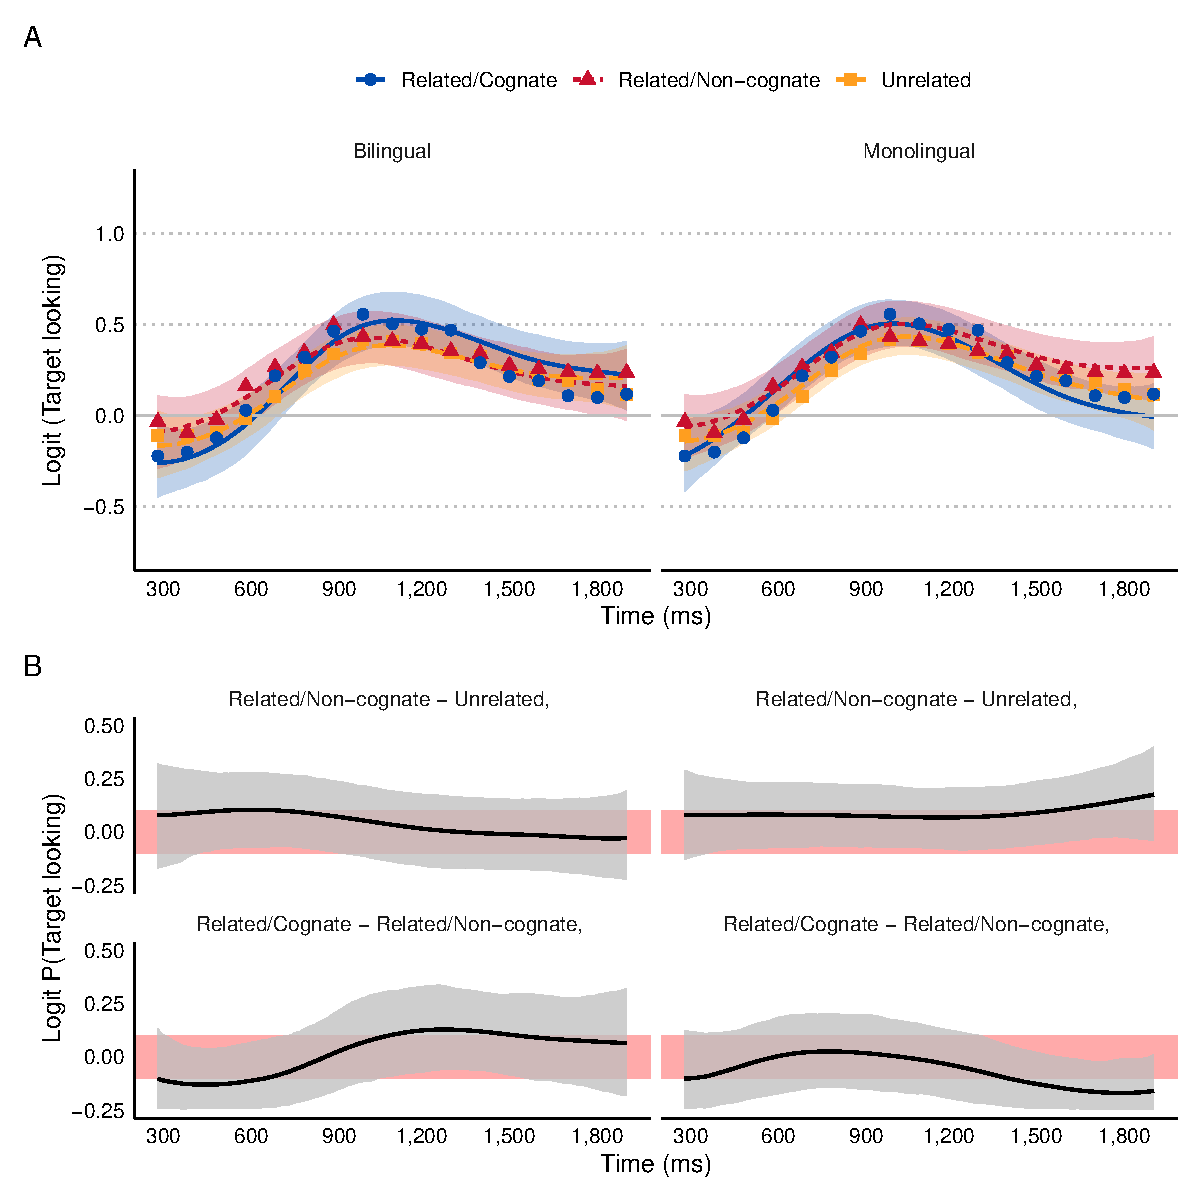
\includegraphics{chapters/03-chapter-3_files/figure-pdf/fig-epreds-1.pdf}

}

\caption{\label{fig-epreds}Time course of target fixations in Study 2.
A) Posterior mean predictions of the time course of target fixation in
the test phase. B) Posterior mean prediction of the time course of the
differences in target looking time between conditions. Intervals
represent the 95\% CrI of the posterior predictions. Lines indicate the
mean of the posterior predictions.}

\end{figure}

\hypertarget{age-and-vocabulary-size-effects-1}{%
\subsubsection{Age and vocabulary size
effects}\label{age-and-vocabulary-size-effects-1}}

A comparison between models including \emph{Age} (\(\mathcal{M}_{1}\)),
\emph{L1 vocabulary} (\(\mathcal{M}_{2}\)), and \emph{Total vocabulary}
(\(\mathcal{M}_{3}\)) against model \(\mathcal{M}_{0}\), which only
included \emph{Age} as a main effect is shown in
Table~\ref{tbl-loos-bcn}. Overall, all models performed equivalently,
with the model \(\mathcal{M}_{2}\) showing slightly better performance.
The equivalent performance of all models suggests that participants'
target looking during the test phase can be predicted with relative
accuracy without taking into account \emph{L1 vocabulary}, or
\emph{Total vocabulary} sizes. We now report the median and 95\% HDI of
the coefficients of \(\mathcal{M}_{2}\), the best-fitting model.

\hypertarget{tbl-loos-bcn}{}
\begin{table}
\caption{\label{tbl-loos-bcn}Leave-one-out cross validation outcomes, comparing the predictive
performance of the models in Study 1. \(ELDP\): sum of expected log
pointwise predictive density for a new data set. \(ELDP_{SE}\): standard
error of the \(ELPD\), which indictes the uncertainty about the
predictive performance for unknown future data. \(\Delta\): pairwise
difference in \(ELPD\) for two models. The difference is computed
relative to the model with lowest \(ELPD\) (best fitting model).
\(\Delta_{SE}\): standard error of component-wise differences of
\emph{ELPD} between two models. }\tabularnewline

\centering
\begin{tabular}{lrrrrr}
\toprule
  & Predictors & $ELDP$ & $ELDP_{SE}$ & $\Delta$ & $\Delta_{SE}$\\
\midrule
$\mathcal{M}_1$ & $\text{Age} \times \text{Condition}$ & -8,469.02 & 73.01 & - & -\\
$\mathcal{M}_0$ & $\text{Age} + \text{Condition}$ & -8,469.15 & 73.02 & -0.13 & 1.11\\
$\mathcal{M}_2$ & $\text{Vocabulary} \times \text{Condition}$ & -8,469.37 & 73.09 & -0.35 & 1.58\\
\bottomrule
\end{tabular}
\end{table}

\hypertarget{discussion-1}{%
\subsection{Discussion}\label{discussion-1}}

Paralleling the results from Study 1 participant' looking behaviour
suggested robust word recognition, regardless of experimental condition,
participant language profile, age, or vocabulary size. Monolinguals and
bilinguals showed equivalent target looking behaviour in
\emph{Unrelated}, \emph{Related/Non-cognate}, and \emph{Related/Cognate}
trials, suggesting that no phonological priming took place, either
within languages or across languages. These results contrast with those
of previous studies using a similar paradigm, which reported
within-language priming effects in same-aged monolinguals (Avila-Varela
et al., 2021; Mani \& Plunkett, 2011a) and younger (Duta et al., 2012;
Mani \& Plunkett, 2010; Styles et al., 2015), and cross-language priming
in adults (Von Holzen \& Mani, 2014).

We anticipated participants' sensitivity to phonological priming to
increase with the size of their lexicon, in the light of previous
studies in which the maturation of the lexicon was associated with
larger phonological interference in word recognition (Chow, Davies, et
al., 2017; Mani \& Plunkett, 2011a). In Study 2, incorporating
participants' age as a predictor in the model in interaction with the
two contrasts of the \emph{Condition} predictor did not increase the
predictive performance of the model. Neither did vocabulary size. This
suggests that the lack of evidence of phonological priming in
participants in this study, either within or across languages, did not
depend of participants lexical development status.

\hypertarget{general-discussion}{%
\section{General discussion}\label{general-discussion}}

In this chapter, we investigated the developmental trajectories of
cross-language co-activation in the initial lexicon. We tested a large
cohort of monolingual and bilingual toddlers in an implicit naming
paradigm, in which we designed three experimental conditions to
manipulate the phonological overlap between the prime and target words
within and across languages. In Unrelated trials, prime and target were
phonologically unrelated in both languages. In Related/Non-cognate
trials, prime and target labels shared phonological onset only in the
dominant language of participants, in which they were tested. In
Related/Cognate trials, the prime label was a cognate: prime and target
labels shared phonological onset in both languages. In Study 1, we
attempted to replicate the original findings by Mani \& Plunkett (2010)
and Mani \& Plunkett (2011a) in a same-aged English monolingual cohort.
We found no evidence of phonological priming. In Study 2, we tested a
cohort of monolingual and bilingual infants learning Catalan, Spanish,
or both, and found similar results, with no evidence of phonological
priming effect in either monolinguals or bilinguals. We did not find any
effect of participants' age or vocabulary size.

The lack of priming effects in Studies 1 and 2 contrasts with previous
findings of within- and cross-language priming using an implicit naming
paradigm. In their seminal study, Mani \& Plunkett (2010) and Mani \&
Plunkett (2011a) reported within-language priming effects in English
monolingual infants. In bilinguals, evidence of cross-linguistic priming
in a implicit naming paradigm was available in adults (Von Holzen \&
Mani, 2014). The priming effects shown in these studies reveal that
infants and adults retrieve phonologically detailed word-forms when
presented with pictures of familiar objects, which later interact with
the subsequent auditory recognition of phonologically related words.
Evidence of such implicit naming is available in infants as young as 14
months. Electrophysiological evidence reported by Duta et al. (2012) and
Styles et al. (2015) suggests that, at this, age, infants lexicalise
name-known pictures presented in silence, and that the generated
phonological form is sensitive to subsequent mispronunciations of the
word. The possibility that infants in the present investigation failed
to retrieve phonological word forms is therefore unlikely.

We consider three scenarios under which implicit naming might have
occurred in the experiments presented in this chapter, but our design
failed to capture it. First, it is be possible that infants in both
Studies 1 and 2 implicitly generated phonological labels for the primes,
but such labels lacked the phonological detail to interact with the
subsequent recognition of a phonologically related target word. This is
unlikely, given that both monolinguals (Bailey \& Plunkett, 2002;
Swingley \& Aslin, 2000; Tamási et al., 2017) and bilinguals
(Ramon-Casas et al., 2009a; Tamási et al., 2016) have been shown to
encode lexical representations with high phonological detail from early
ages.

A second possibility is that participants successfully retrieved a
detailed phonological form of the prime labels, but such forms failed to
interact with target recognition. This would be explained by the lack of
strong associations between phonologically related lexical
representations at these ages. But even if one considers the possibility
that participants in Study 1 failed to show priming effects for this
reason (for instance, the emergence of phonological associations might
follow different trajectories in Catalan-Spanish infants, compared to
English infants), the fact that English monolingual infants in Study 2
failed to show such priming effects contradicts previous findings on the
same population, reporting priming phonological priming effects in even
younger infants (Mani \& Plunkett, 2010, 2011a).

Third, and most likely, the modifications of the implicit naming task in
the present investigation might have reduced the chances of detecting
the anticipated effects. The most critical difference between the
original design of the implicit naming task by Mani and Plunkett and
that of the present study is the absence of a pre-naming phase during
the test phase. Target auditory labels were presented immediately after
the offset of the prime picture. It is possible that such time interval
was too short for participants to retrieve the phonological label of the
prime picture before the target was presented. Such failure to generate
phonological word-forms for prime labels would have prevented
participants in Studies 1 and 2 from being affected by phonological
priming effects during target word recognition.

A difference in the difficulty of the stimuli might have influenced the
results in the present study, compared to those of the original studies.
When designing the stimuli lists, we considered three variables as
indices of word difficult during recognition: lexical frequency, age of
acquisition, and number of phonemes. The distribution of the three
variables was equivalent across the three experimental conditions (see
Table~\ref{tbl-stimuli}), so it is unlikely that such differences
cancelled out a possible priming effect. However, the stricter
limitations under which we build the stimuli lists, might have lead to
out stimuli lists including more difficult words than in the original
study by Mani \& Plunkett (2010). We examined this possibility by
comparing the distributions of the English words included in Study 1,
with those included in Mani \& Plunkett (2010) and Mani \& Plunkett
(2011a) (stimuli lists are identical in both studies). \textbf{?@fig-mp}
shows a comparison between the stimuli lists of the three studies in
lexical frequency and word familiarity at 18 months. Overall, words
included in Mani and Plunkett and in Study 1 have equivalent lexical
frequency, and are know by a similar proportion of English monolinguals
infants, according to the OCDI norms. This is the case for prime and
target words across the related and the unrelated conditions. It is
therefore unlikely that the lack of priming effects in Study 1 is due to
an increased difficulty in the items included.

Another possibility is that participants in the present study had
smaller vocabulary sizes than those of participants in the original
studies. This hypothesis is not easy to investigate, as quantitative
vocabulary sizes were not reported in original studies. A more recent
study by Avila-Varela et al. (2021), in which phonological priming
effects were found associated to participants vocabulary size, did
provide summary statistics for participants vocabulary size scores. This
study tested a cohort of monolingual German infants in a word
recognition task, in which participants in which participants were
presented with auditory primes and targets, which were phonologically
related or unrelated. The authors estimated participants' receptive
vocabulary sizes using the \emph{Fragebogen zur frühkindlichen
Sprachentwicklung} (Szagun et al., 2009), an adaptation of the CDI to
German. Their cohort of participants showed receptive vocabulary sizes
larger than those of participants in the present study. Participants in
Avila-Varela et al. (2021) knew an average of 405.24 (\emph{SD} = 96.29)
at 21 months and 501.97 (\emph{SD} = 73.41) at 24 months, which contrast
with receptive vocabulary sizes of participants in Study 1: 293 at 21
months (\emph{SD} = 71.24), and 304.33 (\emph{SD} = 134.63) at 25
months.

In summary, we aimed to test the language non-selective hypothesis of
lexical access in bilingual toddlers using an adaptation of the implicit
naming paradigm. This adaptation involved target auditory labels
immediately after the offset of prime pictures, instead of presenting
the target labels after a baseline period of 2,000 after the offset of
the prime pictures. In Study 1, we tested English monolinguals (same
population as in the original studies) to establish a baseline to later
test bilingual participants. We attempted to replicate the previously
reported within-language phonological priming effect. We did not find
evidence of such effect, suggesting that our modification of the
original task was unsuccessful. Because data collection was conducted
simultaneously for Studies 1 and 2, data in Catalan-Spanish monolinguals
and bilinguals was available despite the failed replication in Study 1.
In Study 2, we also found null pattern of results, in which neither
monolinguals nor bilinguals showed evidence of within- or cross-language
priming effects. Overall, our results suggest that the change in the
timing of the trial disrupted the dynamics of word recognition in such
way that priming effects were no longer detectable in our adaptation of
the paradigm.

\hypertarget{appendix-d-imputing-vocabulary-sizes}{%
\section{Appendix D: Imputing vocabulary
sizes}\label{appendix-d-imputing-vocabulary-sizes}}

To test the validity of caregivers' estimates of word comprehension in
the vocabulary questionnaires, we compared participants' target looking
for target words reported as acquired, compared to those reported as not
acquired. If parents' responses are accurate, target looking preference
should be stronger in for acquired words. We conducted this analysis by
computing the logit of the probability of target looking at during the
presentation of the target and the distractor pictures for each
participant across conditions, and then across participants. In
Figure~\ref{fig-validity-target}, we report the target looking trends in
the three groups tested in Chapter 3: English monolinguals in Study 1,
Catalan and Spanish monolinguals in Study 2, and Catalan-Spanish
bilinguals in Study 3. Monolinguals and bilinguals in Study 2 showed a
stronger target preference for target words reported as acquired,
compared to words not reported as acquired. The probability of target
looking for acquired targets exceeded zero in monolinguals and
bilinguals, whereas the probability of target looking for targets not
reported as acquired did not exceed zero. These outcomes provide
evidence of concurrent validity for the acquisition estimates of
families in Study 2. The results from participants in Study 1 show a
different patterns, in which participants showed a strong target looking
preference for all target words, reported as acquired or not. This
indicates that families likely underestimated their children's word
comprehension abilities in their vocabulary checklists.

\begin{figure}

{\centering 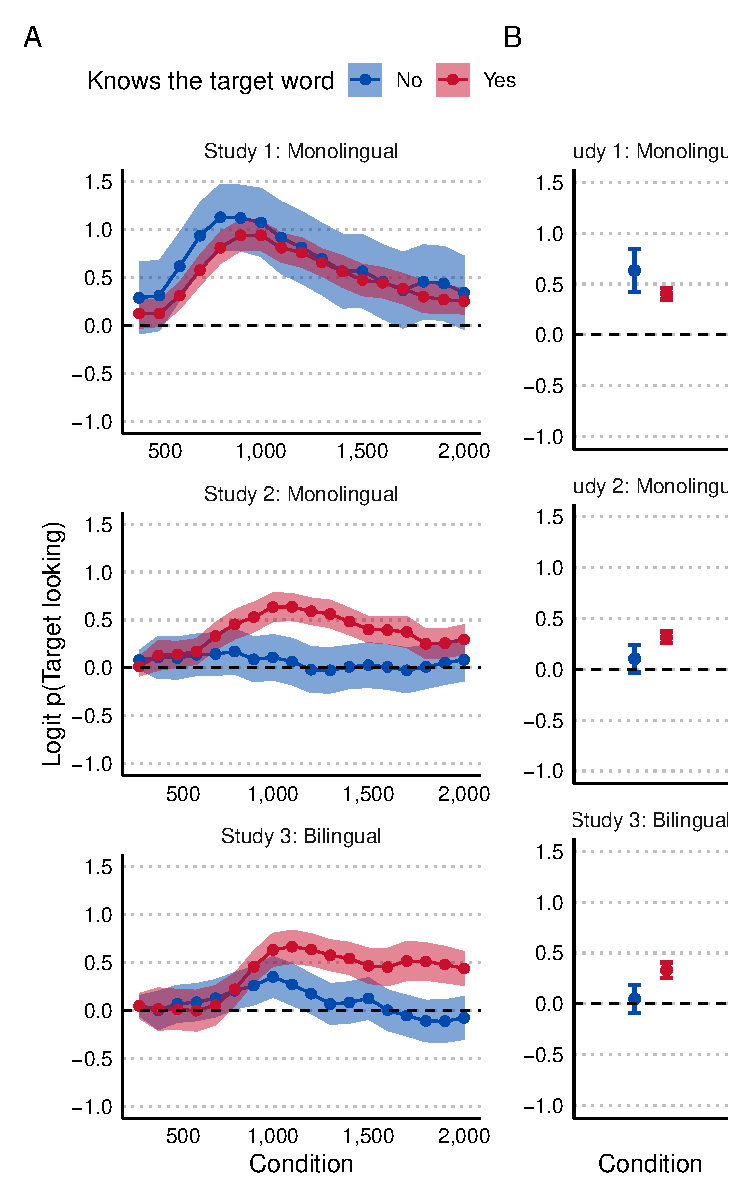
\includegraphics[width=1\textwidth,height=\textheight]{chapters/03-chapter-3_files/figure-pdf/fig-validity-target-1.pdf}

}

\caption{\label{fig-validity-target}Target fixations for words reported
as acquired (red) and for words not reported as acquired (blue) by
caregivers in the vocabulary checklists. (A) Time course of fixations
300 ms after the presentation of the target and distractor pictures,
until the end of the trials. Lines and intervals indicate the mean and
standard error of the mean. (B) Target looking preference, averaged
across the trials. Points and intervals indicate the mean and standard
error of the mean.}

\end{figure}

\newpage{}

\hypertarget{appendix-e-concurrent-validity-of-comprehension-estimates}{%
\section{Appendix E: Concurrent validity of comprehension
estimates}\label{appendix-e-concurrent-validity-of-comprehension-estimates}}

Given the large number of participants in Study 2 whose families failed
to fill in the vocabulary questionnaire in time, we imputed missing
vocabulary sizes to avoid losing their data in subsequent analyses. We
used the \texttt{mice} R package (Buuren \& Groothuis-Oudshoorn, 2011)
to perform single imputations via Bayesian linear regression.
Figure~\ref{fig-vocabulary-imputation} shows the distribution of
observed and imputed vocabulary sizes. Overall, the distribution of
imputed vocabulary sizes was equivalent to the distribution of observed
vocabulary sizes of participants with similar age and language profile.

\begin{figure}

{\centering 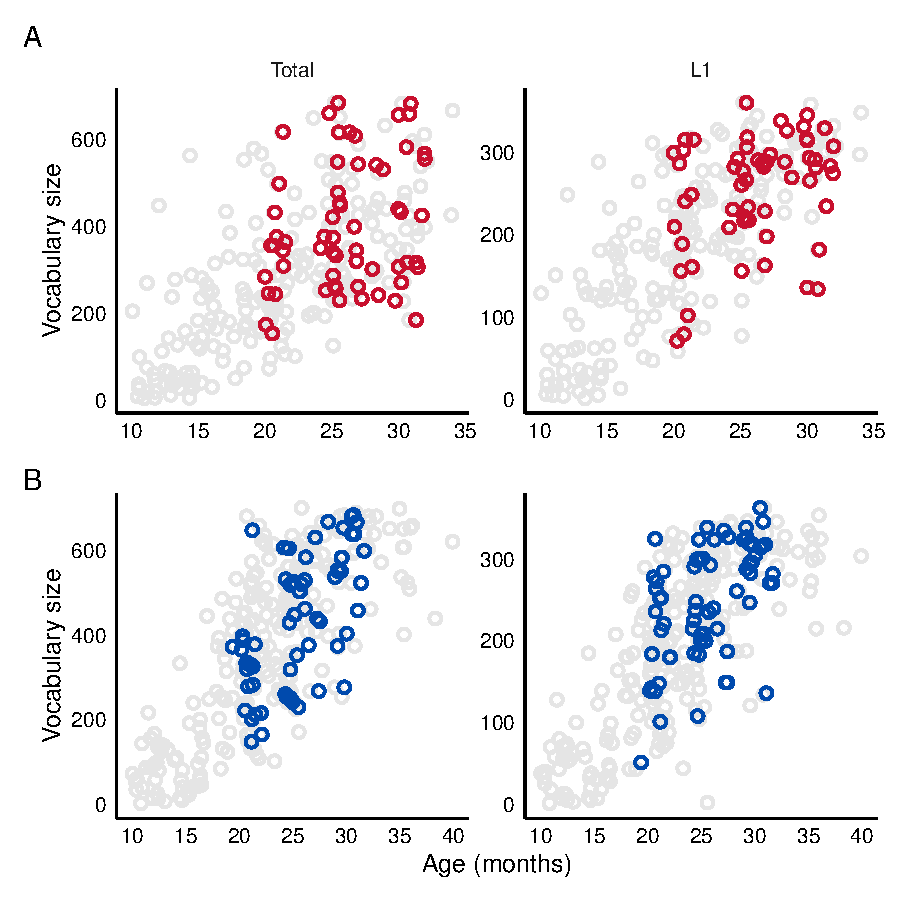
\includegraphics{chapters/03-chapter-3_files/figure-pdf/fig-vocabulary-imputation-1.pdf}

}

\caption{\label{fig-vocabulary-imputation}Imputation of missing
receptive vocabulary size scores in Study 2 for monolinguals (A) and
bilinguals (B). vocabulary size scores are epxressed in raw counts, that
is, the number of words reported by caregivers as acquired. Vocabulary
sizes were imputed from a larger sample of children who provided
responses to the Barcelona Vocabulary Questionnaire. We used
participants' age and language profile to impute scores of participants
wih the same profile. Imputed observations are highlighted in red
(monolinguals) and blue (bilinguals)}

\end{figure}

\newpage{}

\bookmarksetup{startatroot}

\hypertarget{discussion-2}{%
\chapter{Discussion}\label{discussion-2}}

The aim of the present thesis was to investigate the initial bilingual
lexicon. We explored the role of cross-language lexical similarity on
word acquisition, and its possible impact on the dynamics of lexical
access. In this concluding chapter, we summarise the results from
Chapters 2 and 3. We then elaborate on the implications of our findings
on theoretical, and comment on some of the methodological limitations
encountered. We also discuss possible steps to take in future research.
We conclude highlighting the main contributions of the thesis.

\hypertarget{summary-of-results}{%
\section{Summary of results}\label{summary-of-results}}

In Chapter 2, we investigated how cognateness affects word acquisition
in 10-to-32 month-old bilinguals learning Catalan and Spanish. We used
Item Response Theory (IRT) to model the acquisition trajectories of a
large sample of Catalan and Spanish words, and found a facilitation
effect of cognateness on the probability of comprehension and
production. This facilitation was mediated by an \emph{ad hoc} index of
word exposure, which adjusted the lexical frequency of the words for the
dual linguistic input of bilinguals. Low-exposure words benefited more
strongly from their cognate status, whereas words with average or high
exposure were unaffected by their cognate status. We interpreted these
results as evidence in favour of language non-selectivity playing a
central role the initial lexicon. In particular, we suggested that
exposure instances to words in one language contributed, to some extent
as exposure instances to their translation equivalents (TEs).

Our account for the results found in Chapter 2 built on the assumption
that bilingual infants co-activate the TEs in both languages, even
during monolingual situations, in which they hear words in exclusively
one of the languages. Previous experimental work on language
non-selectivity in the initial lexicon relied on paradigms in which
participants are presented with words from the two languages during the
same testing session, introducing them into a bilingual context (Floccia
et al., 2020; Jardak \& Byers-Heinlein, 2019; Singh, 2014; Von Holzen \&
Mani, 2012a). To our knowledge, no previous study had tested whether
language non-selectivity takes place in fully monolingual paradigms. We
addressed this gap in the literature in Chapter 3. We tested language
non-selectivity in infants using an implicit naming paradigm, adapted
from Mani and Plunkett (2010, 2011a). Participants were presented with
an exclusively monolingual task. By manipulating the cognate status of
prime words, and its impact on subsequent recognition of phonologically
related words, we aimed to test whether participants co-activated TEs in
both languages in monolingual situations. Methodological caveats in the
adaptation of the task prevented us from draw conclusions from this
experiment.

\hypertarget{towards-a-model-of-bilingual-vocabulary-growth}{%
\section{Towards a model of bilingual vocabulary
growth}\label{towards-a-model-of-bilingual-vocabulary-growth}}

Differences in the developmental trajectories of word acquisition across
bilingual populations have gained some attention in last decade. It had
been previously established that, on average, bilingual infants learn
words at a similar rate as monolinguals, despite facing a more
challenging word-learning task (Bosch \& Ramon-Casas, 2014;
Byers-Heinlein et al., 2023a; Core et al., 2013; Pearson et al., 1993;
Pearson \& Fernández, 1994; Poulin-Dubois et al., 2013a). An influential
monograph by Floccia, Sambrook, Delle Luche, Kwok, Goslin, White,
Cattani, Sullivan, Abbot‐Smith, et al. (2018) provided evidence for a
possible mechanism behind bilingual word acquisition: bilingual toddlers
learning two lexically similar languages (e.g., English-Dutch) show
larger productive vocabularies than those learning two lexical, less
similar languages (e.g., English-Mandarin). This suggested that some
populations of bilinguals may exploit the similarities between their
languages---particularly, the phonological similarity between TEs---to
acquire words faster (see also Gampe et al., 2021). The authors pointed
at the language non-selective hypothesis of lexical access as the
mechanism behind this cross-language facilitation effect. How the
dynamics of lexical access in the initial lexicon might relate to word
acquisition was still to be addressed.

In Chapter 2, we explored the trajectories of acquisition of cognate and
non-cognate words, and found an earlier age of the former---even after
controlling for lexical frequency, relative language exposure, and word
length---in line with previous findings by Mitchell et al. (2022). This
facilitation effect was stronger in words to which participants were
exposed less often. These results converge with two main predictions
from our proposal. First, the earlier age-of-acquisition for cognates
than for non-cognates is in line with a faster accumulation of learning
instances for cognates. This might be the result of cognate words
receiving stronger co-activation from their TEs than non-cognates. We
suggest that this might have been driven by cognates receiving
additional activation in a higher degree than than non-cognates, because
of their higher phonological similarity. The asymmetry in the size
cognateness facilitation effect between high-exposure and low-exposure
words provides further support for this explanation. Words with lower
lexical frequency or belonging to participants' less dominant language
(in which they receive less input) should benefit more strongly from the
additional co-activation provided by their (more frequently activated)
translation, than higher exposure words, which might receive such
additional co-activation less frequently. This mechanism may explain the
facilitative role of lexical similar reported by Floccia, Sambrook,
Delle Luche, Kwok, Goslin, White, Cattani, Sullivan, Abbot‐Smith, et al.
(2018), and the asymmetry found in the size of such effect between the
English vocabulary and the additional-language vocabulary in their
participants. Since English was the dominant language for most
participants in their sample, it is possible that the increment in
vocabulary size drive by cognates was stronger in the additional
language, leading to a larger facilitation effect of lexical similarity.
In summary, these results have important consequences for current models
of bilingual lexical acquisition.

The present theoretical account makes an important contribution to the
research on the bilingual lexicon. Few models of the bilingual lexicon
have addressed the issue of early lexical acquisition. Instead, previous
modelling efforts have mostly focused on word comprehension and
production in the adult lexicon. Notable exemplars of models of the
adult lexicon are the Revised Hierarchical Model (RHM) (Kroll \&
Stewart, 1994), the Bilingual Interactive Activation (BIA) model and its
revised successor BIA+ (Dijkstra \& Van Heuven, 2002, 2013), BIMOLA
(Grosjean, 1988; Léwy, 2008), SOMBIT (Li et al., 2004; Li \& Farkas,
2002), and BLINCS (Shook \& Marian, 2013). The more recent proposal of
the Multilink model (Dijkstra et al., 2019) integrates features of the
RMH and BIA/BIA+ models to simulate a wide range of experimental
observations in bilingual adults, spanning from the cognate facilitation
effect in word recognition and production, as well as word translation.
These models have provided valuable insight into the structure of the
bilingual lexicon, and the underlying dynamics of word recognition and
production, but have paid little attention to the developmental
dimension of lexical acquisition. Other contributions, like the
Ontogenic Model (Bordag et al., 2022; Gor et al., 2021), BIA-d (a more
development-oriented extension of the BIA/BIA+ model, Grainger et al.,
2010), have delved into the emergence and consolidation of lexical
representations during second language acquisition, still through the
lens of the adult lexicon. In summary, few studies have addressed the
early bilingual lexicon.

One exception is the DevLex-II model by Zhao \& Li (2007), a bilingual
extension of DevLex (Li et al., 2007) focused on monolingual lexical
development. This connectionist model describes how lexical
representations emerge during the simultaneous acquisition of two
languages, and how phonological similarity shapes the structure of the
resulting lexicon. DevLex-II successfully generates plausible patterns
of lexical growth. For instance TEs are mapped together in the
simulations of this model, suggesting that the acquisition of words in
one language is sensitive to the acquisition of their translations in
the other, in line with previous findings (Bilson et al., 2015; R. K.-Y.
Tsui et al., 2022b). Simulations of word comprehension from DevLex-II
also reveal within- and cross-language interference effect at the
semantic and phonological levels, paralleling results in bilingual
children: when the model was presented with a word, related semantic and
phonological representations in both languages competed for selection
(Zhao \& Li, 2013). The case of cognate words was not addressed in this
model.

In Chapter 2, we presented a model of bilingual lexical acquisition. We
also discussed its predictions, and underlying assumptions. In the
following paragraphs, we present a first iteration into the
formalisation of this model, which we have entitled as the Accumulator
Model of Bilingual Lexical Acquisition (AMBLA). As its name indicates,
AMBLA extends the notion of \emph{accumulator} to the bilingual case,
borrowed from accumulator models of language acquisition (Hidaka, 2013;
Kachergis et al., 2022b; Mollica \& Piantadosi, 2017b). The central goal
of AMBLA is to explain the two predictions tested in Chapter 2: that
cognates are acquired earlier than non-cognates, and that this effect is
stronger in the less-dominant language of the childen. To explain how
AMBLA works, we simulate the acquisition trajectories of two
Catalan-Spanish TEs by a bilingual child learning Catalan and Spanish.
The first TE is a cognate (/\textipa{'gat}/--/\textipa{"ga.to}/
{[}cat{]}), and the second is a non-cognate
(/\textipa{"gos}/--/\textipa{"pe.ro"}/). For illustration purposes, we
assume a scenario in which the child is exposed 60\% of the time to
Catalan (dominant language), and 40\% of the time to Spanish
(non-dominant language).

For each word-form, AMBLA generates an estimated age-of-acquisition.
This value indicates the age at which some fixed proportion of the
children in the target popoulation (generally 50\%) have acquired a word
Piñeiro \& Manzano (2000), according to caregivers' reports of word
acquisition (e.g., Fenson et al., 1994, 2007), or the size of naming
effects in word recognition paradigms (Marchman \& Fernald, 2008;
Marchman \& Martínez-Sussmann, 2002). In AMBLA, the age-of-acquisition
is defined as the age at which the child has accumulated a critical
number of learning instances with the word-form. In the following
simulations, we set this threshold at 300. This value was calibrated so
that the scale of the model can be compared to the observed data in
Chapter 2.

In AMBLA, the rate at which a child (\(i\)) accumulates leaning
instances with a word form (\(j\)) is a multiplicative funcion of four
variables (See Equation~\ref{eq-ambla}). First, the child's age
(\(\text{Age}_i\)): the older the child, the more learning instances
they accumulate with the word-form. for interpretability, we expressed
the childs' age in months in the simulation below. A second variable is
the lexical frequency of the word-form (\(\text{Frequency}_j\)): the
child will accumulate learning instances with more frequent words faster
than with less frequent words. We assume that lexical frequency is a
valid indicator of the amount of times child is exposed to a given
word-form per unit of time, and that each exposure contributes one word
learning instance\footnote{Not all learning instances may be effective,
  as the mere exposure to a word-form may not result in the accumulation
  of information about the word and its referent. For simplicity, in the
  presented simulations we assumed that each exposure contributes one
  learning instance.}. We operationalised lexical frequency as the
amount of times a child may encounter a word-form in their speech input
in the time span of a month. Given that this number of exposure
instances may randomly vary from month to month, assumed a Poisson
distribution to generate word exposure counts for each word-form in each
month. For simplicity, we assume identical lexical frequency for all
word-forms by assigning the same parameters for the Poisson distribution
(\(\lambda = 50\), which assumes that the child is most likely to
encounter each word around 50 times per month).

The third variable is the child's relative exposure to the language to
which the word belongs to (\(\text{Exposure}_{ij}\)): children will
accumulate learning instances with words from their higher-exposure
language faster than with words from their lower-exposure language. This
variable takes values from 0 (the child does not receive any exposure to
this language) to 1 (the child only receives exposure to this language).
The child's degree of exposure to all languages must sum up to one.
Finally, the fourth variable is the amount of phonological similarity
between the two TEs (\(\text{Cognateness}_j\)). This score ranges from 0
(no similarity) to 1 (identical cognates), and is calculated using the
Levenshtein similarity, as in Chapter 2.

\begin{equation}\protect\hypertarget{eq-ambla}{}{
\begin{aligned}
\textbf{AMBLA:}\\
\text{AoA}_{ij} &= \{\text{Age}_i \mid y_{ij} = c\}\\
y_{ij} &= \text{Age}_i \cdot \text{Frequency}_j \cdot \text{Exposure}_{ij} \cdot \text{Cognateness}_j\\
\text{Frequency}_j &\sim \text{Poisson}(\lambda) \\
\text{Cognateness}_{j, j_{TE}} &= \text{Levenshtein}(j, j_{TE}) \\\\
\text{Where:} \\
i&: \text{ child} \\
j&: \text{word-form} \\
j_{TE}&: \text{Translation equivalent of word-form } j\\
\text{AoA}_{ij}&: \text{ Age-of-acquisition of word } j \text{ for child } i\\
c&: \text{ Threshold number of learning instances for word acquisition} \\
y_{ij}&: \text{ Learning instances with word } j \text{ accumulated by child } i\\\\
\text{For simulations}&: c = 300 \text{, } \lambda_j = 50 \\
\end{aligned}
}\label{eq-ambla}\end{equation}

Figure~\ref{fig-ambla} illustrates the outcomes of 50 simulations of the
AMBLA model for the two TEs. Overall, the accumulation of learning
instances is faster for the Catalan word-forms than for the Spanish
forms, leading to an earlier age-of-acquisition for the former. This is
an anticipated outcome, as the child is more likely to encounter Catalan
word-forms in their speech input, compared to Spanish word-forms (again,
assuming that lexical frequency is constant for the Catalan and the
Spanish word-forms). This difference in age-of-acquisition between
Catalan and Spanish word-forms is attenuated by their cognate status.
The AMBLA model assumes a cross-talk between word-forms in both
languages, in such way that learning instances for word-forms in one
language may count as well for their TEs, as the result of their
co-activation during speech comprehension. For instance, the Spanish
word-form /\textipa{"ga.to}/ benefits from the learning instances that
its cognate translation /\textipa{"gat}/ receives (both word-forms share
0.75 Levenshtein similarity). The Spanish word-form /\textipa{"pe.ro}/
however, would benefit in a less degree from the learning instances
accumulated by its non-cognate translation /\textipa{"gos}/, given their
low phonological similarity (0.00). In the case of the cognate TE, the
word-form in the language of lower exposure (Spanish) occurs at an
earlier age than in the non-cognate TE, as the result of the language
non-selective accumulation of learning instances across phonological
links.

\newpage

\begin{figure}

{\centering 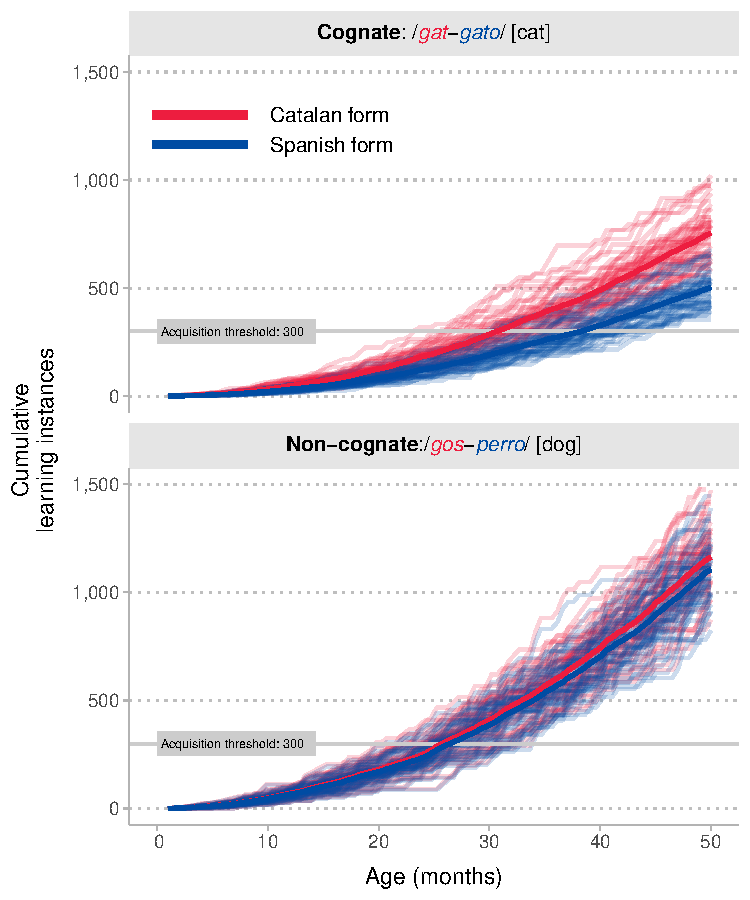
\includegraphics[width=1\textwidth,height=1\textheight]{chapters/04-discussion_files/figure-pdf/fig-ambla-1.pdf}

}

\caption{\label{fig-ambla}Simulations from AMBLA for the acquisition for
two translation equivalents in Catalan and Spanish. Thinner lines
represent 50 simulations for each word-form. Thicker lines indicate the
mean of the simulations for the same word-form. Word-forms in Catalan
are depicted in red. Word-forms in Spanish are depicture in blue. The
X-axis indicates the age of participants in months. The Y-axis indicates
the cumulative learning instances for each word-form. We indicate the
threshold number of learning instances that a word must accumulate to be
acquired with a horizontal grey line.}

\end{figure}

The simulations from AMBLA also reflect the asymmetric facilitation
effect of cognateness on word acquisition. In the cognate TE, the
word-form belonging to the language of lower exposure (Spanish)
benefited from its cognate status more strongly than the Catalan word,
which belonged to the language of higher exposure. These outcomes mirror
the findings in Chapter 2, which provides converging evidence for the
central mechanism of AMBLA: the cross-language accumulation of learning
instances for cognate words. As previously explained, we hypothesis that
the asymmetry in this effect is driven by the fact that word-forms from
the higher-exposure language (which the child encounters more
frequently) provide additional learning instances to their TEs than
word-forms from the lower-exposure language (which the child encounters
less frequently).

The simulations from AMBLA presented above correspond to a first
interation in the formalisation of the model. Future work will be
addressed at refining and expanding its current implementation. The
ultimate goal is to make AMBLA a useful model for generating and testing
quantitative predictions of word age-of-acquisition (Kachergis et al.,
2022b), while keeping a minimal structure and ensuring the
interpretability of its parameters (see Magnuson et al., 2020 for a
similar approach on a minimal model of spoken word recognition). More
generally, we anticipate that a more principled formalisation of the
inner workings of AMBLA may provide a stronger bridge between hypotheses
about lexical development, and the statistical inference conducted on
observations about word acquisition (Guest \& Martin, 2021; Navarro,
2019; Wills et al., 2017).

\hypertarget{methodological-contributions}{%
\section{Methodological
contributions}\label{methodological-contributions}}

A considerable part of the present dissertation has built on a database
of vocabulary data collected from 2020 onwards. To gather this database,
we designed and implemented an \emph{ad hoc} questionnaire the Barcelona
Vocabulary Questionnaire (BVQ) (Garcia-Castro, Ávila-Varela, et al.,
2023b). This questionnaire was filled in by a large sample of families
of monolinguals and bilinguals aged 10 to 32 months, learning Catalan
and Spanish. Collected data included comprehension and production
estimates for individual words in Catalan and Spanish. Queries to the
database can be performed through its associated R package \texttt{bvq}
(\url{https://gongcastro.github.io/bvq}), which provides a sizable
amount of acquisition reports, and may be used to address further
research questions about bilingual lexical development. In addition,
this questionnaire was developed open source software, and all the
materials and code used in process are available at the GitHub
repository (\url{https://github.com/gongcastro/bvq}).

Another contribution of the present dissertation is the modelling
approach adopted throughout Chapters 2 and 3. We highlight two features
of interest. First, we adopted a Bayesian approach to parameter
estimation and statistical inference. This approach provides great
advantages, compared to the more widespread frequentist approach. Among
them, we highlight the possibility to incorporate previous knowledge
about the distribution of parameters of interest in a model, providing a
more stable and efficient computation of the posterior coefficients.
This proved to be a valuable asset in the implementation of complex
multilevel structures for the random effects of the models, which we
describe below. Some participants contributed partial datasets, in which
for particular combinations of levels of the predictors of interested,
few observations were gathered, if any. In these cases, a frequentist
approach would most likely have provided unstable inferences, if not
computational complications (e.g., convergence issues during the
estimation of parameters). Following a Bayesian approach, we specified a
weakly informative prior for the parameters in our models, so that
incoming observations would gradually update the shape of the
distribution of the parameters until data collection concluded. At no
point the parameters of the models provided infeasible estimates, as the
distribution of their parameters was constrained by theoretically
grounded prior distributions.

In Chapter 2, caregivers of many ---but not all of---participants
provided answers about comprehension or production for the same words.
Conversely, the same participant provided such responses to
multiple---but not all of---words. To analyse this type of datasets,
previous studies aggregated scores across items or participants, in
order to avoid violations of the assumption of independence between the
residuals of related observations (e.g., belonging to the same
participant) (Bosch \& Ramon-Casas, 2014; Floccia, Sambrook, Delle
Luche, Kwok, Goslin, White, Cattani, Sullivan, Abbot‐Smith, et al.,
2018). As a consequence, information at participant-level or item-level
was not available in subsequent analyses. On the contrary, in this
dissertation we incorporated the complex data collection design into the
structure of our model in the form of IRT, in which participants and
words were included as crossed random effects in the random effects
structure of the model. Data analysis in Chapter 3 also benefited from
this approach, given its complex data collection design, in which some
participants were tested more than once. In this case, we included
participants and testing sessions as nested random effects. In summary,
the present dissertation benefited from a Bayesian approach to
statistical inference that may be of interest for future research in
language acquisition.

\hypertarget{limitations-and-future-research}{%
\section{Limitations and future
research}\label{limitations-and-future-research}}

One of the main pitfalls encountered in this dissertation was the
experimental caveats in Chapter 3. Our adaptation of the original
implicit naming task by Mani and Plunkett (2010, 2011a) failed to
reproduce the expected results. We introduced some adjustments to the
structure of the trial, in order to maximise the probability of
detecting cross-language priming effects. Such effects are short-lived
and more difficult to detect than within language priming effects. For
this reason, we removed the pre-naming phase of the trial, in which
target and distractor pictures are presented prior to the auditory
target label. This made the presentation of the prime picture and the
target auditory label closer in time. We expected the immediacy of the
presentation of both stimuli to increase of the size of the priming
effect. Instead, this adjustment appeared to disrupt the lexical
retrieval of the prime label, in such way that priming effects were not
observed in any of the experimental conditions. This prevented us from
drawing any conclusions about the presence of such effects in the
initial lexicon from this experiment. Future research should address
whether a longer inter-stimulus interval between the presentation of the
prime and the target would lead to the observation of priming effects.

The present dissertation contributes several open questions. One of them
is if the cognate facilitation effect reported in Chapter 2 is present
in other populations of bilinguals, namely those learning more lexically
dissimilar languages. As mentioned in the Discussion section of Chapter
2, Catalan and Spanish share many cognates. The large amount of cognates
shared by Catalan and Spanish may increase infants' sensitivity to
cross-linguistic phonological similarity during vocabulary acquisition
leading to cognateness playing a more central role than in the case of
infants who encounter fewer cognates in their linguistic input. For
instance, infants learning English and Mandarin, two languages that
share very few cognates, may not be able to exploit cross-language
similarity to boost the acquisition of words in both languages during
language exposure. The approach followed by Floccia, Sambrook, Delle
Luche, Kwok, Goslin, White, Cattani, Sullivan, Abbot‐Smith, et al.
(2018; Floccia et al., 2020; see also Siow et al., 2023) of collecting
data from infants learning a diverse pool of language pairs would be
convenient for addressing this issue.

The evidence provided in Chapter 2 in favour of an earlier
age-of-acquisition of cognates does not address the particular
mechanisms infants may use to accumulate information about word-forms
and their association to their corresponding referents. We used the term
\emph{learning instance} (Mollica \& Piantadosi, 2017a) to refer to
exposures to a word in which infants \emph{may} use to consolidate its
lexical representation. Determining the specific condition under which a
learning instance is effective (i.e., may lead to word learning) falls
out of the scope of the present dissertation. We simply assume that some
learning instances may be effective, and that the number of effective
learning instance is a function of the total number of learning infants
a child encounters on a daily basis. An experimental approach to word
learning, in which the impact of cognateness is investigated, would
provide valuable insights into the mechanisms behind the role of
cross-linguistic similarity on word acquisition.

For instance, a recent study by R. K.-Y. Tsui et al. (2023) provides a
potentially suitable paradigm to investigate the impact of cognateness
on online word learning. The authors designed a word learning task in
which they tested bilingual infants aged 3-to-5 years of age, learning
French and English (in Montreal, Canada), and Spanish and English (in
New Jersey, United States). In the learning phase, participants were
trained to associate novel labels to novel objects. At test,
participants were presented with pairs of objects encountered in the
learning phase, and a label that corresponded to one of them.
Participants were instructed to select the corresponding object in a
touchscreen. Participants completed two blocks of training and test
phases. In the training phase of one block, participants were presented
with sentences labelling the novel objects in both languages in an
interleaved fashion. For instance, in one trial they would be presented
with a novel object, which would be labelled in English (e.g.,
\emph{gasser} in English). In the next trial, they would be presented
with the same object, which this time would be labelled in French (e.g.,
\emph{donquete} in French, or \emph{sasco} in Spanish). This condition
simulated a \emph{language mixing} environment (i.e., children are
exposed to both languages in the same situations, encountering words
from both languages interleaved in speech), to which a sizeable
proportion of bilinguals are exposed (Byers-Heinlein, 2013). In the
training phase of the other block, participants were presented with
consecutive trials labelling the object in the same language, and then
with consecutive trials labelling the object in the other language. This
condition simulated a \emph{one-language-at-a-time} environment.
Overall, participants succeeded at learning the words in both
conditions. This suggests that infants benefit equally from being
exposed to labelling events in alternating languages in an interleaved
fashion (a bilingual environment) and in an synchronous fashion
(monolingual situations).

R. K.-Y. Tsui et al. (2023) used phonologically distinct novel labels
across languages. By extending this paradigm it could be possible to
investigate whether participants learning of the label-referent
associations is facilitated by the degree of phonological between the
TEs. If participants co-activate newly learned TEs in both languages,
word learning should be facilitation more strongly by the repetition of
phonologically similar TEs (i.e., cognates) than from the repetition of
phonologically dissimilar TEs (i.e.~non-cognates). Another variable of
interest for such experimental paradigm could be the lexical similarity
between the two languages being acquired. The two populations of
bilinguals in R. K.-Y. Tsui et al. (2023), ones exposed to French and
English, and the others to Spanish-English, were learning two languages
belonging to two different typological families. At the lexical level
both pairs of languages are relatively distant, compared to languages
belonging to the same family, like Catalan and Spanish. By comparing how
bilinguals process cognates in world learning contexts, depending on the
overall lexical similarity of their languages (e.g., high in the case of
Catalan and Spanish, low in the case of Euskera and Spanish), it could
be possible to investigate how the linguistic input shapes the
strategies followed by bilinguals during early lexical development. In
summary, future steps may involve experimental paradigms to investigate
the mechanisms involved in the cognate facilitation of word acquisition
with more details, and with a finer control of the conditions in which
participants are exposed to the word-forms.

\hypertarget{conclusions}{%
\section{Conclusions}\label{conclusions}}

The present dissertation provides insights into the developing bilingual
lexicon. We provided evidence in favour of a mechanistic account of word
acquisition, in which bilinguals exploit the language non-selectivity of
their lexicon to facilitate the acquisition of cognate words. These
findings have important consequences for the current understanding of
bilingual vocabulary growth, and in particular, the mechanisms
underlying the parallel trajectories of lexical acquisition of
monolinguals and bilinguals.

\clearpage

\bookmarksetup{startatroot}

\hypertarget{bibliography}{%
\chapter*{Bibliography}\label{bibliography}}
\addcontentsline{toc}{chapter}{Bibliography}

\markboth{Bibliography}{Bibliography}

\begingroup

\hypertarget{refs}{}
\begin{CSLReferences}{1}{0}
\leavevmode\vadjust pre{\hypertarget{ref-abboub2016prosodic}{}}%
Abboub, N., Nazzi, T., \& Gervain, J. (2016). Prosodic grouping at
birth. \emph{Brain and Language}, \emph{162}, 46--59.
\url{https://doi.org/10.1016/j.bandl.2016.08.002}

\leavevmode\vadjust pre{\hypertarget{ref-agresti2012categorical}{}}%
Agresti, A. (2012). \emph{Categorical data analysis} (Vol. 792). John
Wiley \& Sons.

\leavevmode\vadjust pre{\hypertarget{ref-albareda2011acquisition}{}}%
Albareda-Castellot, B., Pons, F., \& Sebastián-Gallés, N. (2011). The
acquisition of phonetic categories in bilingual infants: New data from
an anticipatory eye movement paradigm. \emph{Developmental Science},
\emph{14}(2), 395--401.

\leavevmode\vadjust pre{\hypertarget{ref-allopenna1998tracking}{}}%
Allopenna, P. D., Magnuson, J. S., \& Tanenhaus, M. K. (1998). Tracking
the time course of spoken word recognition using eye movements: Evidence
for continuous mapping models. \emph{Journal of Memory and Language},
\emph{38}(4), 419--439.

\leavevmode\vadjust pre{\hypertarget{ref-antovich2018learning}{}}%
Antovich, D. M., \& Graf Estes, K. (2018). Learning across languages:
Bilingual experience supports dual language statistical word
segmentation. \emph{Developmental Science}, \emph{21}(2), e12548.
\url{https://doi.org/10.1111/desc.12548}

\leavevmode\vadjust pre{\hypertarget{ref-arias2009lexical}{}}%
Arias-Trejo, N., \& Plunkett, K. (2009). Lexical--semantic priming
effects during infancy. \emph{Philosophical Transactions of the Royal
Society B: Biological Sciences}, \emph{364}(1536), 3633--3647.

\leavevmode\vadjust pre{\hypertarget{ref-arslan2020formr}{}}%
Arslan, R. C., Walther, M. P., \& Tata, C. S. (2020). Formr: A study
framework allowing for automated feedback generation and complex
longitudinal experience-sampling studies using r. \emph{Behavior
Research Methods}, \emph{52}(1), 376--387.
\url{https://doi.org/10.3758/s13428-019-01236-y}

\leavevmode\vadjust pre{\hypertarget{ref-aslin1981discrimination}{}}%
Aslin, R. N., Pisoni, D. B., Hennessy, B. L., \& Perey, A. J. (1981).
Discrimination of voice onset time by human infants: New findings and
implications for the effects of early experience. \emph{Child
Development}, \emph{52}(4), 1135.

\leavevmode\vadjust pre{\hypertarget{ref-aslin1996models}{}}%
Aslin, R. N., Woodward, J. Z., LaMendola, N. P., \& Bever, T. G. (1996).
Models of word segmentation in fluent maternal speech to infants.
\emph{Signal to Syntax: Bootstrapping from Speech to Grammar in Early
Acquisition}, 117--134.

\leavevmode\vadjust pre{\hypertarget{ref-au1990principle}{}}%
Au, T. K., \& Glusman, M. (1990). The principle of mutual exclusivity in
word learning: To honor or not to honor? \emph{Child Development},
\emph{61}(5), 1474--1490.

\leavevmode\vadjust pre{\hypertarget{ref-avila2021longitudinal}{}}%
Avila-Varela, D. S., Arias-Trejo, N., \& Mani, N. (2021). A longitudinal
study of the role of vocabulary size in priming effects in early
childhood. \emph{Journal of Experimental Child Psychology}, \emph{205},
105071.

\leavevmode\vadjust pre{\hypertarget{ref-bailey2002phonological}{}}%
Bailey, T. M., \& Plunkett, K. (2002). Phonological specificity in early
words. \emph{Cognitive Development}, \emph{17}(2), 1265--1282.
\url{https://doi.org/10.1016/S0885-2014(02)00116-8}

\leavevmode\vadjust pre{\hypertarget{ref-ballem2005phonological}{}}%
Ballem, K. D., \& Plunkett, K. (2005). Phonological specificity in
children at 1; 2. \emph{Journal of Child Language}, \emph{32}(1),
159--173.

\leavevmode\vadjust pre{\hypertarget{ref-barr2008analyzing}{}}%
Barr, D. J. (2008). Analyzing `visual world'eyetracking data using
multilevel logistic regression. \emph{Journal of Memory and Language},
\emph{59}(4), 457--474.

\leavevmode\vadjust pre{\hypertarget{ref-barr2013random}{}}%
Barr, D. J., Levy, R., Scheepers, C., \& Tily, H. J. (2013). Random
effects structure for confirmatory hypothesis testing: Keep it maximal.
\emph{Journal of Memory and Language}, \emph{68}(3), 255--278.

\leavevmode\vadjust pre{\hypertarget{ref-basnight2007differences}{}}%
Basnight-Brown, D. M., \& Altarriba, J. (2007). Differences in semantic
and translation priming across languages: The role of language direction
and language dominance. \emph{Memory \& Cognition}, \emph{35}, 953--965.

\leavevmode\vadjust pre{\hypertarget{ref-bates2013emergence}{}}%
Bates, E., \& Goodman, J. C. (2013). On the emergence of grammar from
the lexicon. In \emph{The emergence of language} (pp. 47--98).
Psychology Press.

\leavevmode\vadjust pre{\hypertarget{ref-bates1994developmental}{}}%
Bates, E., Marchman, V., Thal, D., Fenson, L., Dale, P., Reznick, J. S.,
Reilly, J., \& Hartung, J. (1994). Developmental and stylistic variation
in the composition of early vocabulary. \emph{Journal of Child
Language}, \emph{21}(1), 85--123.

\leavevmode\vadjust pre{\hypertarget{ref-bedore2005conceptual}{}}%
Bedore, L. M., Peña, E. D., García, M., \& Cortez, C. (2005).
\emph{Conceptual versus monolingual scoring}.

\leavevmode\vadjust pre{\hypertarget{ref-bergelson2020comprehension}{}}%
Bergelson, E. (2020). The comprehension boost in early word learning:
Older infants are better learners. \emph{Child Development
Perspectives}, \emph{14}(3), 142--149.
\url{https://doi.org/10.1111/cdep.12373}

\leavevmode\vadjust pre{\hypertarget{ref-bergelson20126}{}}%
Bergelson, E., \& Swingley, D. (2012a). At 6--9 months, human infants
know the meanings of many common nouns. \emph{Proceedings of the
National Academy of Sciences}, \emph{109}(9), 3253--3258.

\leavevmode\vadjust pre{\hypertarget{ref-bergelson2012months}{}}%
Bergelson, E., \& Swingley, D. (2012b). At 6--9 months, human infants
know the meanings of many common nouns. \emph{Proceedings of the
National Academy of Sciences}, \emph{109}(9), 3253--3258.
\url{https://doi.org/10.1073/pnas.1113380109}

\leavevmode\vadjust pre{\hypertarget{ref-bergelson2015early}{}}%
Bergelson, E., \& Swingley, D. (2015). Early word comprehension in
infants: Replication and extension. \emph{Language Learning and
Development}, \emph{11}(4), 369--380.
\url{https://doi.org/10.1080/15475441.2014.979387}

\leavevmode\vadjust pre{\hypertarget{ref-bertoncini1987discrimination}{}}%
Bertoncini, J., Bijeljac-Babic, R., Blumstein, S. E., \& Mehler, J.
(1987). Discrimination in neonates of very short CVs. \emph{The Journal
of the Acoustical Society of America}, \emph{82}(1), 31--37.

\leavevmode\vadjust pre{\hypertarget{ref-best1994emergence}{}}%
Best, C. T. et al. (1994). The emergence of native-language phonological
influences in infants: A perceptual assimilation model. \emph{The
Development of Speech Perception: The Transition from Speech Sounds to
Spoken Words}, \emph{167}(224), 233--277.

\leavevmode\vadjust pre{\hypertarget{ref-bialystok2009bilingualism}{}}%
Bialystok, E. (2009). Bilingualism: The good, the bad, and the
indifferent. \emph{Bilingualism: Language and Cognition}, \emph{12}(1),
3--11.

\leavevmode\vadjust pre{\hypertarget{ref-bilson2015semantic}{}}%
Bilson, S., Yoshida, H., Tran, C. D., Woods, E. A., \& Hills, T. T.
(2015). Semantic facilitation in bilingual first language acquisition.
\emph{Cognition}, \emph{140}, 122--134.

\leavevmode\vadjust pre{\hypertarget{ref-blom2020cross}{}}%
Blom, E., Boerma, T., Bosma, E., Cornips, L., Heuij, K. van den, \&
Timmermeister, M. (2020a). Cross-language distance influences receptive
vocabulary outcomes of bilingual children. \emph{First Language},
\emph{40}(2), 151--171.

\leavevmode\vadjust pre{\hypertarget{ref-blom2020crosslanguage}{}}%
Blom, E., Boerma, T., Bosma, E., Cornips, L., Heuij, K. van den, \&
Timmermeister, M. (2020b). Cross-language distance influences receptive
vocabulary outcomes of bilingual children. \emph{First Language},
\emph{40}(2), 151--171. \url{https://doi.org/10.1177/0142723719892794}

\leavevmode\vadjust pre{\hypertarget{ref-bloom2002children}{}}%
Bloom, P. (2002). \emph{How children learn the meanings of words}. MIT
press.

\leavevmode\vadjust pre{\hypertarget{ref-bobb2020co}{}}%
Bobb, S. C., Von Holzen, K., Mayor, J., Mani, N., \& Carreiras, M.
(2020). Co-activation of the L2 during L1 auditory processing: An ERP
cross-modal priming study. \emph{Brain and Language}, \emph{203},
104739.

\leavevmode\vadjust pre{\hypertarget{ref-boersma2001speak}{}}%
Boersma, P., \& Van Heuven, V. (2001). Speak and unSpeak with PRAAT.
\emph{Glot International}, \emph{5}(9/10), 341--347.

\leavevmode\vadjust pre{\hypertarget{ref-bordag2022ontogenesis}{}}%
Bordag, D., Gor, K., \& Opitz, A. (2022). Ontogenesis model of the L2
lexical representation. \emph{Bilingualism: Language and Cognition},
\emph{25}(2), 185--201.

\leavevmode\vadjust pre{\hypertarget{ref-bosch2013rapid}{}}%
Bosch, L., Figueras, M., Teixidó, M., \& Ramon-Casas, M. (2013). Rapid
gains in segmenting fluent speech when words match the rhythmic unit:
Evidence from infants acquiring syllable-timed languages.
\emph{Frontiers in Psychology}, \emph{4}.
\url{https://www.frontiersin.org/articles/10.3389/fpsyg.2013.00106}

\leavevmode\vadjust pre{\hypertarget{ref-bosch2014first}{}}%
Bosch, L., \& Ramon-Casas, M. (2014). First translation equivalents in
bilingual toddlers' expressive vocabulary: Does form similarity matter?
\emph{International Journal of Behavioral Development}, \emph{38}(4),
317--322. \url{https://doi.org/10.1177/0165025414532559}

\leavevmode\vadjust pre{\hypertarget{ref-bosch2001evidence}{}}%
Bosch, L., \& Sebastian-Galles, N. (2001). Evidence of early language
discrimination abilities in infants from bilingual environments.
\emph{Infancy}, \emph{2}(1), 29--49.
\url{https://doi.org/10.1207/S15327078IN0201_3}

\leavevmode\vadjust pre{\hypertarget{ref-bosch1997native}{}}%
Bosch, L., \& Sebastián-Gallés, N. (1997). Native-language recognition
abilities in 4-month-old infants from monolingual and bilingual
environments. \emph{Cognition}, \emph{65}(1), 33--69.

\leavevmode\vadjust pre{\hypertarget{ref-bosch2003simultaneous}{}}%
Bosch, L., \& Sebastián-Gallés, N. (2003). Simultaneous bilingualism and
the perception of a language-specific vowel contrast in the first year
of life. \emph{Language and Speech}, \emph{46}(2), 217--243.

\leavevmode\vadjust pre{\hypertarget{ref-bosma2019longitudinal}{}}%
Bosma, E., Blom, E., Hoekstra, E., \& Versloot, A. (2019). A
longitudinal study on the gradual cognate facilitation effect in
bilingual children's frisian receptive vocabulary. \emph{International
Journal of Bilingual Education and Bilingualism}, \emph{22}(4),
371--385. \url{https://doi.org/10.1080/13670050.2016.1254152}

\leavevmode\vadjust pre{\hypertarget{ref-bosma2020cognate}{}}%
Bosma, E., \& Nota, N. (2020). Cognate facilitation in frisian--dutch
bilingual children's sentence reading: An eye-tracking study.
\emph{Journal of Experimental Child Psychology}, \emph{189}, 104699.

\leavevmode\vadjust pre{\hypertarget{ref-brainard1997psychophysics}{}}%
Brainard, D. H., \& Vision, S. (1997). The psychophysics toolbox.
\emph{Spatial Vision}, \emph{10}(4), 433--436.

\leavevmode\vadjust pre{\hypertarget{ref-burkner2017brms}{}}%
Bürkner, P.-C. (2017). Brms: An r package for bayesian multilevel models
using stan. \emph{Journal of Statistical Software}, \emph{80}, 1--28.
\url{https://doi.org/10.18637/jss.v080.i01}

\leavevmode\vadjust pre{\hypertarget{ref-burns2007development}{}}%
Burns, T. C., Yoshida, K. A., Hill, K., \& Werker, J. F. (2007). The
development of phonetic representation in bilingual and monolingual
infants. \emph{Applied Psycholinguistics}, \emph{28}(3), 455--474.

\leavevmode\vadjust pre{\hypertarget{ref-buuren2011mice}{}}%
Buuren, S. van, \& Groothuis-Oudshoorn, K. (2011). Mice: Multivariate
imputation by chained equations in r. \emph{Journal of Statistical
Software}, \emph{45}(1), 1--67.
\url{https://doi.org/10.18637/jss.v045.i03}

\leavevmode\vadjust pre{\hypertarget{ref-byers2013parental}{}}%
Byers-Heinlein, K. (2013). Parental language mixing: Its measurement and
the relation of mixed input to young bilingual children's vocabulary
size. \emph{Bilingualism: Language and Cognition}, \emph{16}(1), 32--48.

\leavevmode\vadjust pre{\hypertarget{ref-byers2015methods}{}}%
Byers-Heinlein, K. (2015). \emph{Methods for studying infant
bilingualism}.

\leavevmode\vadjust pre{\hypertarget{ref-byers2010roots}{}}%
Byers-Heinlein, K., Burns, T. C., \& Werker, J. F. (2010). The roots of
bilingualism in newborns. \emph{Psychological Science}, \emph{21}(3),
343--348.

\leavevmode\vadjust pre{\hypertarget{ref-byers2023sometimes}{}}%
Byers-Heinlein, K., Gonzalez-Barrero, A. M., Schott, E., \& Killam, H.
(2023a). Sometimes larger, sometimes smaller: Measuring vocabulary in
monolingual and bilingual infants and toddlers. \emph{First Language},
\emph{0}(0), 01427237231204167.
\url{https://doi.org/10.1177/01427237231204167}

\leavevmode\vadjust pre{\hypertarget{ref-byers-heinlein2023sometimes}{}}%
Byers-Heinlein, K., Gonzalez-Barrero, A. M., Schott, E., \& Killam, H.
(2023b). Sometimes larger, sometimes smaller: Measuring vocabulary in
monolingual and bilingual infants and toddlers. \emph{First Language},
\emph{0}(0), 01427237231204167.
\url{https://doi.org/10.1177/01427237231204167}

\leavevmode\vadjust pre{\hypertarget{ref-byers2020maple}{}}%
Byers-Heinlein, K., Schott, E., Gonzalez-Barrero, A. M., Brouillard, M.,
Dubé, D., Jardak, A., Laoun-Rubenstein, A., Mastroberardino, M.,
Morin-Lessard, E., Iliaei, S. P., et al. (2020). MAPLE: A multilingual
approach to parent language estimates. \emph{Bilingualism: Language and
Cognition}, \emph{23}(5), 951--957.

\leavevmode\vadjust pre{\hypertarget{ref-byers2021multilab}{}}%
Byers-Heinlein, K., Tsui, A. S. M., Bergmann, C., Black, A. K., Brown,
A., Carbajal, M. J., Durrant, S., Fennell, C. T., Fiévet, A.-C., Frank,
M. C., et al. (2021). A multilab study of bilingual infants: Exploring
the preference for infant-directed speech. \emph{Advances in Methods and
Practices in Psychological Science}, \emph{4}(1), 2515245920974622.

\leavevmode\vadjust pre{\hypertarget{ref-byers-heinlein2021multilab}{}}%
Byers-Heinlein, K., Tsui, A. S. M., Bergmann, C., Black, A. K., Brown,
A., Carbajal, M. J., \& Wermelinger. (2021). A multilab study of
bilingual infants: Exploring the preference for infant-directed speech.
\emph{Advances in Methods and Practices in Psychological Science},
\emph{4}(1).

\leavevmode\vadjust pre{\hypertarget{ref-campbell2022scope}{}}%
Campbell, J., \& Hall, D. G. (2022). The scope of infants' early object
word extensions. \emph{Cognition}, \emph{228}, 105210.

\leavevmode\vadjust pre{\hypertarget{ref-can2013long}{}}%
Can, D. D., Ginsburg-Block, M., Golinkoff, R. M., \& Hirsh-Pasek, K.
(2013). A long-term predictive validity study: Can the CDI short form be
used to predict language and early literacy skills four years later?
\emph{Journal of Child Language}, \emph{40}(4), 821--835.

\leavevmode\vadjust pre{\hypertarget{ref-caramazza1997many}{}}%
Caramazza, A. (1997). How many levels of processing are there in lexical
access? \emph{Cognitive Neuropsychology}, \emph{14}(1), 177--208.

\leavevmode\vadjust pre{\hypertarget{ref-carpenter2017stan}{}}%
Carpenter, B., Gelman, A., Hoffman, M. D., Lee, D., Goodrich, B.,
Betancourt, M., Brubaker, M., Guo, J., Li, P., \& Riddell, A. (2017).
Stan : A probabilistic programming language. \emph{Journal of
Statistical Software}, \emph{76}(1).
\url{https://doi.org/10.18637/jss.v076.i01}

\leavevmode\vadjust pre{\hypertarget{ref-cattani2014much}{}}%
Cattani, A., Abbot-Smith, K., Farag, R., Krott, A., Arreckx, F., Dennis,
I., \& Floccia, C. (2014). How much exposure to english is necessary for
a bilingual toddler to perform like a monolingual peer in language
tests? \emph{International Journal of Language \& Communication
Disorders}, \emph{49}(6), 649--671.

\leavevmode\vadjust pre{\hypertarget{ref-chow2017spokenword}{}}%
Chow, J., Aimola Davies, A., \& Plunkett, K. (2017). Spoken-word
recognition in 2-year-olds: The tug of war between phonological and
semantic activation. \emph{Journal of Memory and Language}, \emph{93},
104--134. \url{https://doi.org/10.1016/j.jml.2016.08.004}

\leavevmode\vadjust pre{\hypertarget{ref-chow2017spoken}{}}%
Chow, J., Davies, A. A., \& Plunkett, K. (2017). Spoken-word recognition
in 2-year-olds: The tug of war between phonological and semantic
activation. \emph{Journal of Memory and Language}, \emph{93}, 104--134.

\leavevmode\vadjust pre{\hypertarget{ref-christophe1996bootstrapping}{}}%
Christophe, A., \& Dupoux, E. (1996). \emph{Bootstrapping lexical
acquisition: The role of prosodic structure}.

\leavevmode\vadjust pre{\hypertarget{ref-collins1975spreading}{}}%
Collins, A. M., \& Loftus, E. F. (1975). A spreading-activation theory
of semantic processing. \emph{Psychological Review}, \emph{82}(6), 407.

\leavevmode\vadjust pre{\hypertarget{ref-colome2001lexical}{}}%
Colomé, À. (2001). Lexical activation in bilinguals' speech production:
Language-specific or language-independent? \emph{Journal of Memory and
Language}, \emph{45}(4), 721--736.

\leavevmode\vadjust pre{\hypertarget{ref-cook2016fuzzy}{}}%
Cook, S. V., Pandža, N. B., Lancaster, A. K., \& Gor, K. (2016). Fuzzy
nonnative phonolexical representations lead to fuzzy form-to-meaning
mappings. \emph{Frontiers in Psychology}, \emph{7}, 1345.

\leavevmode\vadjust pre{\hypertarget{ref-cooper1990preference}{}}%
Cooper, R. P., \& Aslin, R. N. (1990). Preference for infant-directed
speech in the first month after birth. \emph{Child Development},
\emph{61}(5), 1584--1595.

\leavevmode\vadjust pre{\hypertarget{ref-core2013total}{}}%
Core, C., Hoff, E., Rumiche, R., \& Señor, M. (2013). Total and
conceptual vocabulary in spanish--english bilinguals from 22 to 30
months: Implications for assessment. \emph{Journal of Speech, Language,
and Hearing Research}, \emph{56}(5), 1637--1649.
\url{https://doi.org/10.1044/1092-4388(2013/11-0044)}

\leavevmode\vadjust pre{\hypertarget{ref-costa2000cognate}{}}%
Costa, A., Caramazza, A., \& Sebastian-Galles, N. (2000). The cognate
facilitation effect: Implications for models of lexical access.
\emph{Journal of Experimental Psychology: Learning, Memory, and
Cognition}, \emph{26}, 1283--1296.
\url{https://doi.org/10.1037/0278-7393.26.5.1283}

\leavevmode\vadjust pre{\hypertarget{ref-costa1999lexical}{}}%
Costa, A., Miozzo, M., \& Caramazza, A. (1999). Lexical selection in
bilinguals: Do words in the bilingual's two lexicons compete for
selection? \emph{Journal of Memory and Language}, \emph{41}(3),
365--397.

\leavevmode\vadjust pre{\hypertarget{ref-costa2014does}{}}%
Costa, A., \& Sebastián-Gallés, N. (2014). How does the bilingual
experience sculpt the brain? \emph{Nature Reviews Neuroscience},
\emph{15}(5), 336--345.

\leavevmode\vadjust pre{\hypertarget{ref-cutler1990exploiting}{}}%
Cutler, A. (1990). Exploiting prosodic probabilities in speech
segmentation. In \emph{Cognitive models of speech processing:
Psycholinguistic and computational perspectives} (pp. 105--121). MIT
Press.

\leavevmode\vadjust pre{\hypertarget{ref-cutler1988role}{}}%
Cutler, A., \& Norris, D. (1988). The role of strong syllables in
segmentation for lexical access. \emph{Journal of Experimental
Psychology: Human Perception and Performance}, \emph{14}(1), 113.

\leavevmode\vadjust pre{\hypertarget{ref-cutler2006asymmetric}{}}%
Cutler, A., Weber, A., \& Otake, T. (2006). Asymmetric mapping from
phonetic to lexical representations in second-language listening.
\emph{Journal of Phonetics}, \emph{34}(2), 269--284.

\leavevmode\vadjust pre{\hypertarget{ref-dale1991validity}{}}%
Dale, P. S. (1991). The validity of a parent report measure of
vocabulary and syntax at 24 months. \emph{Journal of Speech, Language,
and Hearing Research}, \emph{34}(3), 565--571.

\leavevmode\vadjust pre{\hypertarget{ref-de2020lexical}{}}%
De Anda, S., \& Friend, M. (2020). Lexical-semantic development in
bilingual toddlers at 18 and 24 months. \emph{Frontiers in Psychology},
\emph{11}, 508363.

\leavevmode\vadjust pre{\hypertarget{ref-de1991lexical}{}}%
De Groot, A. M., \& Nas, G. L. (1991). Lexical representation of
cognates and noncognates in compound bilinguals. \emph{Journal of Memory
and Language}, \emph{30}(1), 90--123.

\leavevmode\vadjust pre{\hypertarget{ref-de2006early}{}}%
De Houwer, A., Bornstein, M. H., \& De Coster, S. (2006). Early
understanding of two words for the same thing: A CDI study of lexical
comprehension in infant bilinguals. \emph{International Journal of
Bilingualism}, \emph{10}(3), 331--347.

\leavevmode\vadjust pre{\hypertarget{ref-de2014bilingual}{}}%
De Houwer, A., Bornstein, M. H., \& Putnick, D. L. (2014). A
bilingual--monolingual comparison of young children's vocabulary size:
Evidence from comprehension and production. \emph{Applied
Psycholinguistics}, \emph{35}(6), 1189--1211.

\leavevmode\vadjust pre{\hypertarget{ref-deanda2016language}{}}%
DeAnda, S., Bosch, L., Poulin-Dubois, D., Zesiger, P., \& Friend, M.
(2016). The language exposure assessment tool: Quantifying language
exposure in infants and children. \emph{Journal of Speech, Language, and
Hearing Research}, \emph{59}(6), 1346--1356.

\leavevmode\vadjust pre{\hypertarget{ref-deanda2018lexical}{}}%
DeAnda, S., Hendrickson, K., Zesiger, P., Poulin-Dubois, D., \& Friend,
M. (2018). Lexical access in the second year: A study of monolingual and
bilingual vocabulary development. \emph{Bilingualism: Language and
Cognition}, \emph{21}(2), 314--327.

\leavevmode\vadjust pre{\hypertarget{ref-decasper1980human}{}}%
DeCasper, A. J., \& Fifer, W. P. (1980). Of human bonding: Newborns
prefer their mothers' voices. \emph{Science}, \emph{208}(4448),
1174--1176.

\leavevmode\vadjust pre{\hypertarget{ref-decasper1994fetal}{}}%
DeCasper, A. J., Lecanuet, J.-P., Busnel, M.-C., Granier-Deferre, C., \&
Maugeais, R. (1994). Fetal reactions to recurrent maternal speech.
\emph{Infant Behavior and Development}, \emph{17}(2), 159--164.

\leavevmode\vadjust pre{\hypertarget{ref-dell1986spreading}{}}%
Dell, G. S. (1986). A spreading-activation theory of retrieval in
sentence production. \emph{Psychological Review}, \emph{93}(3), 283.

\leavevmode\vadjust pre{\hypertarget{ref-delleluche2015methodological}{}}%
Delle Luche, C., Durrant, S., Poltrock, S., \& Floccia, C. (2015). A
methodological investigation of the intermodal preferential looking
paradigm: Methods of analyses, picture selection and data rejection
criteria. \emph{Infant Behavior \& Development}, \emph{40}, 151--172.
\url{https://doi.org/10.1016/j.infbeh.2015.05.005}

\leavevmode\vadjust pre{\hypertarget{ref-dijkstra1999recognition}{}}%
Dijkstra, T., Grainger, J., \& van Heuven, W. J. B. (1999). Recognition
of cognates and interlingual homographs: The neglected role of
phonology. \emph{Journal of Memory and Language}, \emph{41}(4),
496--518. https://doi.org/\url{https://doi.org/10.1006/jmla.1999.2654}

\leavevmode\vadjust pre{\hypertarget{ref-dijkstra2010cross}{}}%
Dijkstra, T., Miwa, K., Brummelhuis, B., Sappelli, M., \& Baayen, H.
(2010). How cross-language similarity and task demands affect cognate
recognition. \emph{Journal of Memory and Language}, \emph{62}(3),
284--301.

\leavevmode\vadjust pre{\hypertarget{ref-dijkstra2002architecture}{}}%
Dijkstra, T., \& Van Heuven, W. J. (2002). The architecture of the
bilingual word recognition system: From identification to decision.
\emph{Bilingualism: Language and Cognition}, \emph{5}(3), 175--197.

\leavevmode\vadjust pre{\hypertarget{ref-dijkstra2013bia}{}}%
Dijkstra, T., \& Van Heuven, W. J. (2013). The BIA model and bilingual
word recognition. In \emph{Localist connectionist approaches to human
cognition} (pp. 189--225). Psychology Press.

\leavevmode\vadjust pre{\hypertarget{ref-dijkstra2019multilink}{}}%
Dijkstra, T., Wahl, A., Buytenhuijs, F., Van Halem, N., Al-Jibouri, Z.,
De Korte, M., \& Rekké, S. (2019). Multilink: A computational model for
bilingual word recognition and word translation. \emph{Bilingualism:
Language and Cognition}, \emph{22}(4), 657--679.

\leavevmode\vadjust pre{\hypertarget{ref-dipietro2013physiological}{}}%
DiPietro, J. A., Voegtline, K. M., Costigan, K. A., Aguirre, F.,
Kivlighan, K., \& Chen, P. (2013). Physiological reactivity of pregnant
women to evoked fetal startle. \emph{Journal of Psychosomatic Research},
\emph{75}(4), 321--326.

\leavevmode\vadjust pre{\hypertarget{ref-dufour1995matching}{}}%
Dufour, R., \& Kroll, J. F. (1995). Matching words to concepts in two
languages: A test of the concept mediation model of bilingual
representation. \emph{Memory \& Cognition}, \emph{23}(2), 166--180.

\leavevmode\vadjust pre{\hypertarget{ref-dunabeitia2009masked}{}}%
Duñabeitia, J. A., Perea, M., \& Carreiras, M. (2009). Masked
translation priming effects with highly proficient simultaneous
bilinguals. \emph{Experimental Psychology}.

\leavevmode\vadjust pre{\hypertarget{ref-duta2012erp}{}}%
Duta, M., Styles, S., \& Plunkett, K. (2012). ERP correlates of
unexpected word forms in a picture--word study of infants and adults.
\emph{Developmental Cognitive Neuroscience}, \emph{2}(2), 223--234.

\leavevmode\vadjust pre{\hypertarget{ref-duyck2005translation}{}}%
Duyck, W. (2005). Translation and associative priming with cross-lingual
pseudohomophones: Evidence for nonselective phonological activation in
bilinguals. \emph{Journal of Experimental Psychology: Learning, Memory,
and Cognition}, \emph{31}(6), 1340.

\leavevmode\vadjust pre{\hypertarget{ref-duyck2009translation}{}}%
Duyck, W., \& Warlop, N. (2009). Translation priming between the native
language and a second language: New evidence from dutch-french
bilinguals. \emph{Experimental Psychology}, \emph{56}(3), 173--179.

\leavevmode\vadjust pre{\hypertarget{ref-ecklund1996asymmetric}{}}%
Ecklund-Flores, L., \& Turkewitz, G. (1996). Asymmetric headturning to
speech and nonspeech in human newborns. \emph{Developmental
Psychobiology}, \emph{29}(3), 205--217.

\leavevmode\vadjust pre{\hypertarget{ref-eggermont2011morphological}{}}%
Eggermont, J. J., \& Moore, J. K. (2011). Morphological and functional
development of the auditory nervous system. In \emph{Human auditory
development} (pp. 61--105). Springer.

\leavevmode\vadjust pre{\hypertarget{ref-eimas1971speech}{}}%
Eimas, P. D., Siqueland, E. R., Jusczyk, P., \& Vigorito, J. (1971).
Speech perception in infants. \emph{Science}, \emph{171}(3968),
303--306. \url{https://doi.org/10.1126/science.171.3968.303}

\leavevmode\vadjust pre{\hypertarget{ref-2018els}{}}%
\emph{Els usos lingüístics de la població de catalunya}. (2018).
Generalitat de Catalunya.
\url{https://llengua.gencat.cat/web/.content/documents/dadesestudis/altres/arxius/dossier-eulp-2018.pdf}

\leavevmode\vadjust pre{\hypertarget{ref-fabian2016investigating}{}}%
Fabian, A. P. (2016). \emph{Investigating vocabulary abilities in
bilingual portuguese-english-speaking children}.

\leavevmode\vadjust pre{\hypertarget{ref-feldman2005concurrent}{}}%
Feldman, H. M., Dale, P. S., Campbell, T. F., Colborn, D. K.,
Kurs-Lasky, M., Rockette, H. E., \& Paradise, J. L. (2005). Concurrent
and predictive validity of parent reports of child language at ages 2
and 3 years. \emph{Child Development}, \emph{76}(4), 856--868.
\url{https://doi.org/10.1111/j.1467-8624.2005.00882.x}

\leavevmode\vadjust pre{\hypertarget{ref-fenson2007macarthurbates}{}}%
Fenson, L. et al. (2007). \emph{{MacArthur}-bates communicative
development inventories}. Paul H. Brookes Publishing Company Baltimore,
{MD}.

\leavevmode\vadjust pre{\hypertarget{ref-fenson1994variability}{}}%
Fenson, L., Dale, P. S., Reznick, J. S., Bates, E., Thal, D. J.,
Pethick, S. J., Tomasello, M., Mervis, C. B., \& Stiles, J. (1994).
Variability in early communicative development. \emph{Monographs of the
Society for Research in Child Development}, \emph{59}(5), i--185.
\url{https://doi.org/10.2307/1166093}

\leavevmode\vadjust pre{\hypertarget{ref-fernald2013ses}{}}%
Fernald, A., Marchman, V. A., \& Weisleder, A. (2013). SES differences
in language processing skill and vocabulary are evident at 18 months.
\emph{Developmental Science}, \emph{16}(2), 234--248.

\leavevmode\vadjust pre{\hypertarget{ref-fernald1998rapid}{}}%
Fernald, A., Pinto, J. P., Swingley, D., Weinberg, A., \& McRoberts, G.
W. (1998). Rapid gains in speed of verbal processing by infants in the
2nd year. \emph{Psychological Science}, \emph{9}(3), 228--231.

\leavevmode\vadjust pre{\hypertarget{ref-fernald2001half}{}}%
Fernald, A., Swingley, D., \& Pinto, J. P. (2001). When half a word is
enough: Infants can recognize spoken words using partial phonetic
information. \emph{Child Development}, \emph{72}(4), 1003--1015.

\leavevmode\vadjust pre{\hypertarget{ref-floccia2020translation}{}}%
Floccia, C., Delle Luche, C., Lepadatu, I., Chow, J., Ratnage, P., \&
Plunkett, K. (2020). Translation equivalent and cross-language semantic
priming in bilingual toddlers. \emph{Journal of Memory and Language},
\emph{112}, 104086.

\leavevmode\vadjust pre{\hypertarget{ref-floccia2018vocabulary}{}}%
Floccia, C., Sambrook, T. D., Delle Luche, C., Kwok, R., Goslin, J.,
White, L., Cattani, A., Sullivan, E., Abbot-Smith, K., Krott, A., et al.
(2018). \emph{Vocabulary of 2-year-olds learning learning english and an
additional language: Norms and effects of linguistic distance}.

\leavevmode\vadjust pre{\hypertarget{ref-floccia2018introduction}{}}%
Floccia, C., Sambrook, T. D., Delle Luche, C., Kwok, R., Goslin, J.,
White, L., Cattani, A., Sullivan, E., Abbot‐Smith, K., Krott, A., Mills,
D., Rowland, C., Gervain, J., \& Plunkett, K. (2018). I: introduction.
\emph{Monographs of the Society for Research in Child Development},
\emph{83}(1), 7--29. \url{https://doi.org/10.1111/mono.12348}

\leavevmode\vadjust pre{\hypertarget{ref-forbes2019infants}{}}%
Forbes, S. H., \& Plunkett, K. (2019). Infants show early comprehension
of basic color words. \emph{Developmental Psychology}, \emph{55}(2),
240.

\leavevmode\vadjust pre{\hypertarget{ref-fourtassi2020growth}{}}%
Fourtassi, A., Bian, Y., \& Frank, M. C. (2020). The growth of
children's semantic and phonological networks: Insight from 10
languages. \emph{Cognitive Science}, \emph{44}(7), e12847.
\url{https://doi.org/10.1111/cogs.12847}

\leavevmode\vadjust pre{\hypertarget{ref-frank2017wordbank}{}}%
Frank, M. C., Braginsky, M., Yurovsky, D., \& Marchman, V. A. (2017).
Wordbank: An open repository for developmental vocabulary data.
\emph{Journal of Child Language}, \emph{44}(3), 677--694.
\url{https://doi.org/10.1017/S0305000916000209}

\leavevmode\vadjust pre{\hypertarget{ref-frank2021variability}{}}%
Frank, M. C., Braginsky, M., Yurovsky, D., \& Marchman, V. A. (2021).
\emph{Variability and consistency in early language learning: The
wordbank project}. {MIT} Press.

\leavevmode\vadjust pre{\hypertarget{ref-friederici1993phonotactic}{}}%
Friederici, A. D., \& Wessels, J. M. I. (1993). Phonotactic knowledge of
word boundaries and its use in infant speech perception.
\emph{Perception \& Psychophysics}, \emph{54}(3), 287--295.
\url{https://doi.org/10.3758/BF03205263}

\leavevmode\vadjust pre{\hypertarget{ref-friedrich2005lexical}{}}%
Friedrich, M., \& Friederici, A. D. (2005a). Lexical priming and
semantic integration reflected in the event-related potential of
14-month-olds. \emph{Neuroreport}, \emph{16}(6), 653--656.

\leavevmode\vadjust pre{\hypertarget{ref-friedrich2005phonotactic}{}}%
Friedrich, M., \& Friederici, A. D. (2005b). Phonotactic knowledge and
lexical-semantic processing in one-year-olds: Brain responses to words
and nonsense words in picture contexts. \emph{Journal of Cognitive
Neuroscience}, \emph{17}(11), 1785--1802.

\leavevmode\vadjust pre{\hypertarget{ref-gampe2018bilex}{}}%
Gampe, A., Kurthen, I., \& Daum, M. M. (2018). BILEX: A new tool
measuring bilingual children's lexicons and translational equivalents.
\emph{First Language}, \emph{38}(3), 263--283.

\leavevmode\vadjust pre{\hypertarget{ref-gampe2021does}{}}%
Gampe, A., Quick, A. E., \& Daum, M. M. (2021). Does linguistic
similarity affect early simultaneous bilingual language acquisition?
\emph{Journal of Language Contact}, \emph{13}(3), 482--500.

\leavevmode\vadjust pre{\hypertarget{ref-ganger2004reexamining}{}}%
Ganger, J., \& Brent, M. R. (2004). Reexamining the vocabulary spurt.
\emph{Developmental Psychology}, \emph{40}(4), 621.

\leavevmode\vadjust pre{\hypertarget{ref-garcia2023cognate}{}}%
Garcia-Castro, G., Avila-Varela, D., Castillejo, I., \&
Sebastian-Galles, N. (2023). \emph{Cognate beginnings to bilingual
lexical acquisition}.

\leavevmode\vadjust pre{\hypertarget{ref-garcia-castro2023bvq}{}}%
Garcia-Castro, G., Ávila-Varela, D. S., \& Sebastian-Galles, N. (2023a).
\emph{Bvq: Barcelona vocabulary questionnaire database and helper
functions}. \url{https://gongcastro.github.io/bvq}

\leavevmode\vadjust pre{\hypertarget{ref-garcia2023bvq}{}}%
Garcia-Castro, G., Ávila-Varela, D. S., \& Sebastian-Galles, N. (2023b).
\emph{Bvq: Barcelona vocabulary questionnaire database and helper
functions}. \url{https://gongcastro.github.io/bvq}

\leavevmode\vadjust pre{\hypertarget{ref-gelman2020regression}{}}%
Gelman, A., Hill, J., \& Vehtari, A. (2020). \emph{Regression and other
stories}. Cambridge University Press.

\leavevmode\vadjust pre{\hypertarget{ref-gelman1992inference}{}}%
Gelman, A., \& Rubin, D. B. (1992). Inference from iterative simulation
using multiple sequences. \emph{Statistical Science}, \emph{7}(4),
457--472. \url{https://www.jstor.org/stable/2246093}

\leavevmode\vadjust pre{\hypertarget{ref-gervain2018role}{}}%
Gervain, J. (2018). The role of prenatal experience in language
development. \emph{Current Opinion in Behavioral Sciences}, \emph{21},
62--67.

\leavevmode\vadjust pre{\hypertarget{ref-giezen2016language}{}}%
Giezen, M. R., \& Emmorey, K. (2016). Language co-activation and lexical
selection in bimodal bilinguals: Evidence from picture--word
interference. \emph{Bilingualism: Language and Cognition}, \emph{19}(2),
264--276.

\leavevmode\vadjust pre{\hypertarget{ref-giguere2022bilingual}{}}%
Giguere, D., \& Hoff, E. (2022). Bilingual development in the receptive
and expressive domains: They differ. \emph{International Journal of
Bilingual Education and Bilingualism}, \emph{25}(10), 3849--3858.
\url{https://doi.org/10.1080/13670050.2022.2087039}

\leavevmode\vadjust pre{\hypertarget{ref-gillen2021tapping}{}}%
Gillen, N. A., Siow, S., Lepadatu, I., Sucevic, J., Plunkett, K., \&
Duta, M. (2021). \emph{Tapping into the potential of remote
developmental research: Introducing the {OxfordBabylab} app}.
{PsyArXiv}. \url{https://doi.org/10.31234/osf.io/kxhmw}

\leavevmode\vadjust pre{\hypertarget{ref-gimeno2021cross}{}}%
Gimeno-Martínez, M., Mädebach, A., \& Baus, C. (2021a). Cross-linguistic
interactions across modalities: Effects of the oral language on sign
production. \emph{Bilingualism: Language and Cognition}, \emph{24}(4),
779--790.

\leavevmode\vadjust pre{\hypertarget{ref-gimeno-martinez2021crosslinguistic}{}}%
Gimeno-Martínez, M., Mädebach, A., \& Baus, C. (2021b). Cross-linguistic
interactions across modalities: Effects of the oral language on sign
production. \emph{Bilingualism: Language and Cognition}, \emph{24}(4),
779--790. \url{https://doi.org/10.1017/S1366728921000171}

\leavevmode\vadjust pre{\hypertarget{ref-goldfield1990early}{}}%
Goldfield, B. A., \& Reznick, J. S. (1990). Early lexical acquisition:
Rate, content, and the vocabulary spurt*. \emph{Journal of Child
Language}, \emph{17}(1), 171--183.
\url{https://doi.org/10.1017/S0305000900013167}

\leavevmode\vadjust pre{\hypertarget{ref-gonzalez-barrero2020bilingual}{}}%
Gonzalez-Barrero, A. M., Schott, E., \& Byers-Heinlein, K. (2020).
\emph{Bilingual adjusted vocabulary: A developmentally-informed
bilingual vocabulary measure}. {PsyArXiv}.
\url{https://doi.org/10.31234/osf.io/x7s4u}

\leavevmode\vadjust pre{\hypertarget{ref-goodman2008does}{}}%
Goodman, J. C., Dale, P. S., \& Li, P. (2008). Does frequency count?
Parental input and the acquisition of vocabulary. \emph{Journal of Child
Language}, \emph{35}(3), 515--531.

\leavevmode\vadjust pre{\hypertarget{ref-goodsitt1993perceptual}{}}%
Goodsitt, J. V., Morgan, J. L., \& Kuhl, P. K. (1993). Perceptual
strategies in prelingual speech segmentation. \emph{Journal of Child
Language}, \emph{20}(2), 229--252.

\leavevmode\vadjust pre{\hypertarget{ref-gor2021fuzzy}{}}%
Gor, K., Cook, S., Bordag, D., Chrabaszcz, A., \& Opitz, A. (2021).
Fuzzy lexical representations in adult second language speakers.
\emph{Frontiers in Psychology}, \emph{12}, 732030.

\leavevmode\vadjust pre{\hypertarget{ref-gout2004phonological}{}}%
Gout, A., Christophe, A., \& Morgan, J. L. (2004). Phonological phrase
boundaries constrain lexical access II. Infant data. \emph{Journal of
Memory and Language}, \emph{51}(4), 548--567.

\leavevmode\vadjust pre{\hypertarget{ref-grainger1998masked}{}}%
Grainger, J. (1998). Masked priming by translation equivalents in
proficient bilinguals. \emph{Language and Cognitive Processes},
\emph{13}(6), 601--623.

\leavevmode\vadjust pre{\hypertarget{ref-grainger2010re}{}}%
Grainger, J., Midgley, K., \& Holcomb, P. J. (2010). Re-thinking the
bilingual interactive-activation model from a developmental perspective
(BIA-d). \emph{Language Acquisition Across Linguistic and Cognitive
Systems}, \emph{52}, 267--283.

\leavevmode\vadjust pre{\hypertarget{ref-groot1992determinants}{}}%
Groot, A. M. de. (1992). Determinants of word translation. \emph{Journal
of Experimental Psychology: Learning, Memory, and Cognition},
\emph{18}(5).

\leavevmode\vadjust pre{\hypertarget{ref-grosjean1980spoken}{}}%
Grosjean, F. (1980). Spoken word recognition processes and the gating
paradigm. \emph{Perception \& Psychophysics}, \emph{28}(4), 267--283.

\leavevmode\vadjust pre{\hypertarget{ref-grosjean1988exploring}{}}%
Grosjean, F. (1988). Exploring the recognition of guest words in
bilingual speech. \emph{Language and Cognitive Processes}, \emph{3}(3),
233--274.

\leavevmode\vadjust pre{\hypertarget{ref-grosjean1997bilingual}{}}%
Grosjean, F. (1997). The bilingual individual. \emph{Interpreting},
\emph{2}(1-2), 163--187.

\leavevmode\vadjust pre{\hypertarget{ref-grosjean2021extent}{}}%
Grosjean, F. (2021). The extent of bilingualism. \emph{Life as a
Bilingual}, 27--39.

\leavevmode\vadjust pre{\hypertarget{ref-guest2021computational}{}}%
Guest, O., \& Martin, A. E. (2021). How computational modeling can force
theory building in psychological science. \emph{Perspectives on
Psychological Science}, \emph{16}(4), 789--802.

\leavevmode\vadjust pre{\hypertarget{ref-halle1994emergence}{}}%
Hallé, P. A., \& Boysson-Bardies, B. de. (1994). Emergence of an early
receptive lexicon: Infants' recognition of words. \emph{Infant Behavior
and Development}, \emph{17}(2), 119--129.

\leavevmode\vadjust pre{\hypertarget{ref-halle1996format}{}}%
Hallé, P. A., \& Boysson-Bardies, B. de. (1996). The format of
representation of recognized words in infants' early receptive lexicon.
\emph{Infant Behavior and Development}, \emph{19}(4), 463--481.

\leavevmode\vadjust pre{\hypertarget{ref-hamilton2000infant}{}}%
Hamilton, A., Plunkett, K., \& Schafer, G. (2000). Infant vocabulary
development assessed with a british communicative development inventory.
\emph{Journal of Child Language}, \emph{27}(3), 689--705.

\leavevmode\vadjust pre{\hypertarget{ref-havy2016phonetic}{}}%
Havy, M., Bouchon, C., \& Nazzi, T. (2016). Phonetic processing when
learning words: The case of bilingual infants. \emph{International
Journal of Behavioral Development}, \emph{40}(1), 41--52.
\url{https://doi.org/10.1177/0165025415570646}

\leavevmode\vadjust pre{\hypertarget{ref-heeringa2003norwegian}{}}%
Heeringa, W., \& Gooskens, C. (2003). Norwegian dialects examined
perceptually and acoustically. \emph{Computers and the Humanities},
\emph{37}(3), 293--315. \url{https://doi.org/10.1023/A:1025087115665}

\leavevmode\vadjust pre{\hypertarget{ref-hidaka2013computational}{}}%
Hidaka, S. (2013). A computational model associating learning process,
word attributes, and age of acquisition. \emph{{PLOS} {ONE}},
\emph{8}(11), e76242. \url{https://doi.org/10.1371/journal.pone.0076242}

\leavevmode\vadjust pre{\hypertarget{ref-hirsh1996intermodal}{}}%
Hirsh-Pasek, K., \& Golinkoff, R. M. (1996). \emph{The intermodal
preferential looking paradigm: A window onto emerging language
comprehension.}

\leavevmode\vadjust pre{\hypertarget{ref-hoff2003specificity}{}}%
Hoff, E. (2003). The specificity of environmental influence:
Socioeconomic status affects early vocabulary development via maternal
speech. \emph{Child Development}, \emph{74}(5), 1368--1378.

\leavevmode\vadjust pre{\hypertarget{ref-hoff2012dual}{}}%
Hoff, E., Core, C., Place, S., Rumiche, R., Señor, M., \& Parra, M.
(2012). Dual language exposure and early bilingual development*.
\emph{Journal of Child Language}, \emph{39}(1), 1--27.
\url{https://doi.org/10.1017/S0305000910000759}

\leavevmode\vadjust pre{\hypertarget{ref-hoshino2008cognate}{}}%
Hoshino, N., \& Kroll, J. F. (2008). Cognate effects in picture naming:
Does cross-language activation survive a change of script?
\emph{Cognition}, \emph{106}(1), 501--511.
\url{https://doi.org/10.1016/j.cognition.2007.02.001}

\leavevmode\vadjust pre{\hypertarget{ref-hoshino2010erp}{}}%
Hoshino, N., Midgley, K. J., Holcomb, P. J., \& Grainger, J. (2010). An
ERP investigation of masked cross-script translation priming.
\emph{Brain Research}, \emph{1344}, 159--172.

\leavevmode\vadjust pre{\hypertarget{ref-houston2000role}{}}%
Houston, D. M., \& Jusczyk, P. W. (2000). The role of talker-specific
information in word segmentation by infants. \emph{Journal of
Experimental Psychology: Human Perception and Performance},
\emph{26}(5), 1570.

\leavevmode\vadjust pre{\hypertarget{ref-houston-price2007discrepancy}{}}%
Houston-Price, C., Mather, E., \& Sakkalou, E. (2007). Discrepancy
between parental reports of infants' receptive vocabulary and infants'
behaviour in a preferential looking task. \emph{Journal of Child
Language}, \emph{34}(4), 701--724.
\url{https://doi.org/10.1017/S0305000907008124}

\leavevmode\vadjust pre{\hypertarget{ref-huettig2007tug}{}}%
Huettig, F., \& McQueen, J. M. (2007). The tug of war between
phonological, semantic and shape information in language-mediated visual
search. \emph{Journal of Memory and Language}, \emph{57}(4), 460--482.

\leavevmode\vadjust pre{\hypertarget{ref-hurtado2014relative}{}}%
Hurtado, N., Grüter, T., Marchman, V. A., \& Fernald, A. (2014).
Relative language exposure, processing efficiency and vocabulary in
spanish--english bilingual toddlers. \emph{Bilingualism: Language and
Cognition}, \emph{17}(1), 189--202.
\url{https://doi.org/10.1017/S136672891300014X}

\leavevmode\vadjust pre{\hypertarget{ref-hurtado2007spoken}{}}%
Hurtado, N., Marchman, V. A., \& Fernald, A. (2007). Spoken word
recognition by latino children learning spanish as their first language.
\emph{Journal of Child Language}, \emph{34}(2), 227--249.

\leavevmode\vadjust pre{\hypertarget{ref-hustad2021speech}{}}%
Hustad, K. C., Mahr, T. J., Natzke, P., \& Rathouz, P. J. (2021). Speech
development between 30 and 119 months in typical children i:
Intelligibility growth curves for single-word and multiword productions.
\emph{Journal of Speech, Language, and Hearing Research}, \emph{64}(10),
3707--3719. \url{https://doi.org/10.1044/2021_JSLHR-21-00142}

\leavevmode\vadjust pre{\hypertarget{ref-jackendoff2002words}{}}%
Jackendoff, R. (2002). Combinatoriality. In \emph{Foundations of
language} (p. 39). Oxford University Press.

\leavevmode\vadjust pre{\hypertarget{ref-jackson1993early}{}}%
Jackson-Maldonado, D., Thal, D., Marchman, V., Bates, E., \&
Gutierrez-Clellen, V. (1993). Early lexical development in
spanish-speaking infants and toddlers. \emph{Journal of Child Language},
\emph{20}(3), 523--549.

\leavevmode\vadjust pre{\hypertarget{ref-jahn2001vocabulary}{}}%
Jahn-Samilo, J., Goodman, J., Bates, E., \& Sweet, M. (2001). Vocabulary
learning in children from 8 to 30 months of age: A comparison of
parental report and laboratory measures. \emph{Manuscript Submitted for
Publication}.

\leavevmode\vadjust pre{\hypertarget{ref-jardak2019labels}{}}%
Jardak, A., \& Byers-Heinlein, K. (2019). Labels or concepts? The
development of semantic networks in bilingual two-year-olds. \emph{Child
Development}, \emph{90}(2), e212--e229.

\leavevmode\vadjust pre{\hypertarget{ref-jusczyk1995infants}{}}%
Jusczyk, P. W., \& Aslin, R. N. (1995). Infants' detection of the sound
patterns of words in fluent speech. \emph{Cognitive Psychology},
\emph{29}(1), 1--23. \url{https://doi.org/10.1006/cogp.1995.1010}

\leavevmode\vadjust pre{\hypertarget{ref-jusczyk1992perception}{}}%
Jusczyk, P. W., Hirsh-Pasek, K., Nelson, D. G. K., Kennedy, L. J.,
Woodward, A., \& Piwoz, J. (1992). Perception of acoustic correlates of
major phrasal units by young infants. \emph{Cognitive Psychology},
\emph{24}(2), 252--293.

\leavevmode\vadjust pre{\hypertarget{ref-jusczyk1994infants}{}}%
Jusczyk, P. W., Luce, P. A., \& Charles-Luce, J. (1994). Infants'
sensitivity to phonotactic patterns in the native language.
\emph{Journal of Memory and Language}, \emph{33}(5), 630--645.

\leavevmode\vadjust pre{\hypertarget{ref-kachergis2022toward}{}}%
Kachergis, G., Marchman, V. A., \& Frank, M. C. (2022a). Toward a
{``standard model''} of early language learning. \emph{Current
Directions in Psychological Science}, \emph{31}(1), 20--27.

\leavevmode\vadjust pre{\hypertarget{ref-kachergis2022standard}{}}%
Kachergis, G., Marchman, V. A., \& Frank, M. C. (2022b). Toward a
{``standard model''} of early language learning. \emph{Current
Directions in Psychological Science}, \emph{31}(1), 20--27.
\url{https://doi.org/10.1177/09637214211057836}

\leavevmode\vadjust pre{\hypertarget{ref-kern2007lexicon}{}}%
Kern, S. (2007). Lexicon development in french-speaking infants.
\emph{First Language}, \emph{27}(3), 227--250.

\leavevmode\vadjust pre{\hypertarget{ref-kern2019lexical}{}}%
Kern, S., Valente, D., \& Santos, C. dos. (2019). Lexical development in
bilingual french/portuguese speaking toddlers: Vocabulary size and
language dominance. \emph{Journal of Monolingual and Bilingual Speech},
\emph{1}(2), 206--224.

\leavevmode\vadjust pre{\hypertarget{ref-kisilevsky2009fetal}{}}%
Kisilevsky, B. S., Hains, S. M., Brown, C. A., Lee, C. T.,
Cowperthwaite, B., Stutzman, S. S., Swansburg, M. L., Lee, K., Xie, X.,
Huang, H., et al. (2009). Fetal sensitivity to properties of maternal
speech and language. \emph{Infant Behavior and Development},
\emph{32}(1), 59--71.

\leavevmode\vadjust pre{\hypertarget{ref-kleiner2007s}{}}%
Kleiner, M., Brainard, D., \& Pelli, D. (2007). \emph{What's new in
psychtoolbox-3?}

\leavevmode\vadjust pre{\hypertarget{ref-krauska2023moving}{}}%
Krauska, A., \& Lau, E. (2023). Moving away from lexicalism in
psycho-and neuro-linguistics. \emph{Frontiers in Language Sciences},
\emph{2}, 1125127.

\leavevmode\vadjust pre{\hypertarget{ref-kroll2010revised}{}}%
Kroll, J. F., Hell, J. G. V., Tokowicz, N., \& Green, D. W. (2010). The
revised hierarchical model: A critical review and assessment*.
\emph{Bilingualism: Language and Cognition}, \emph{13}(3), 373--381.
\url{https://doi.org/10.1017/S136672891000009X}

\leavevmode\vadjust pre{\hypertarget{ref-kroll2017bilingual}{}}%
Kroll, J. F., \& Ma, F. (2017). The bilingual lexicon. \emph{The
Handbook of Psycholinguistics}, 294--319.

\leavevmode\vadjust pre{\hypertarget{ref-kroll1994category}{}}%
Kroll, J. F., \& Stewart, E. (1994). Category interference in
translation and picture naming: Evidence for asymmetric connections
between bilingual memory representations. \emph{Journal of Memory and
Language}, \emph{33}(2), 149--174.

\leavevmode\vadjust pre{\hypertarget{ref-kruschke2014doing}{}}%
Kruschke, J. (2014). \emph{Doing bayesian data analysis: A tutorial with
r, JAGS, and stan}.

\leavevmode\vadjust pre{\hypertarget{ref-kruschke2018bayesian}{}}%
Kruschke, J. K., \& Liddell, T. M. (2018). The bayesian new statistics:
Hypothesis testing, estimation, meta-analysis, and planning from a
bayesian perspective. \emph{Psychonomic Bulletin \&Review}, \emph{25},
178--206. \url{https://doi.org/10.3758/s13423-016-1221-4}

\leavevmode\vadjust pre{\hypertarget{ref-kuhl1991human}{}}%
Kuhl, P. K. (1991). Human adults and human infants show a {``perceptual
magnet effect''} for the prototypes of speech categories, monkeys do
not. \emph{Perception \& Psychophysics}, \emph{50}(2), 93--107.

\leavevmode\vadjust pre{\hypertarget{ref-kuhl2006infants}{}}%
Kuhl, P. K., Stevens, E., Hayashi, A., Deguchi, T., Kiritani, S., \&
Iverson, P. (2006). Infants show a facilitation effect for native
language phonetic perception between 6 and 12 months.
\emph{Developmental Science}, \emph{9}(2), F13--F21.

\leavevmode\vadjust pre{\hypertarget{ref-kukona2011time}{}}%
Kukona, A., Fang, S.-Y., Aicher, K. A., Chen, H., \& Magnuson, J. S.
(2011). The time course of anticipatory constraint integration.
\emph{Cognition}, \emph{119}(1), 23--42.

\leavevmode\vadjust pre{\hypertarget{ref-legacy2018vocabulary}{}}%
Legacy, J., Zesiger, P., Friend, M., \& Poulin-Dubois, D. (2018).
Vocabulary size and speed of word recognition in very young
french--english bilinguals: A longitudinal study. \emph{Bilingualism:
Language and Cognition}, \emph{21}(1), 137--149.

\leavevmode\vadjust pre{\hypertarget{ref-levelt1989language}{}}%
Levelt, W. (1989). \emph{Language production}. MIT Press Cambridge, MA.

\leavevmode\vadjust pre{\hypertarget{ref-levenshtein1966binary}{}}%
Levenshtein, V. I. (1966). Binary codes capable of correcting deletions,
insertions, and reversals. \emph{Soviet Physics-Doklady}, \emph{10},
707--710.

\leavevmode\vadjust pre{\hypertarget{ref-lewy2008lewy}{}}%
Léwy, N. (2008). The l{é}wy and grosjean BIMOLA model. \emph{Studying
Bilinguals}, 201--210.

\leavevmode\vadjust pre{\hypertarget{ref-li20023self}{}}%
Li, P., \& Farkas, I. (2002). 3 a self-organizing connectionist model of
bilingual processing. In \emph{Advances in psychology} (Vol. 134, pp.
59--85). Elsevier.

\leavevmode\vadjust pre{\hypertarget{ref-li2004early}{}}%
Li, P., Farkas, I., \& MacWhinney, B. (2004). Early lexical development
in a self-organizing neural network. \emph{Neural Networks},
\emph{17}(8-9), 1345--1362.

\leavevmode\vadjust pre{\hypertarget{ref-li2007dynamic}{}}%
Li, P., Zhao, X., \& Mac Whinney, B. (2007). Dynamic self-organization
and early lexical development in children. \emph{Cognitive Science},
\emph{31}(4), 581--612.

\leavevmode\vadjust pre{\hypertarget{ref-vanderloo2014stringdist}{}}%
Loo, M. P. J. van der. (2014). The stringdist package for approximate
string matching. \emph{The R Journal}, \emph{6}(1), 111--122.
\url{https://doi.org/10.32614/RJ-2014-011}

\leavevmode\vadjust pre{\hypertarget{ref-luce1998recognizing}{}}%
Luce, P. A., \& Pisoni, D. B. (1998). Recognizing spoken words: The
neighborhood activation model. \emph{Ear and Hearing}, \emph{19}(1), 1.

\leavevmode\vadjust pre{\hypertarget{ref-luce1990similarity}{}}%
Luce, P. A., Pisoni, D. B., \& Goldinger, S. D. (1990). \emph{Similarity
neighborhoods of spoken words.}

\leavevmode\vadjust pre{\hypertarget{ref-macwhinney2000childes}{}}%
MacWhinney, B. (2000). \emph{The {CHILDES} project: The database} (Vol.
2). Psychology Press.

\leavevmode\vadjust pre{\hypertarget{ref-magnuson2020earshot}{}}%
Magnuson, J. S., You, H., Luthra, S., Li, M., Nam, H., Escabi, M.,
Brown, K., Allopenna, P. D., Theodore, R. M., Monto, N., et al. (2020).
EARSHOT: A minimal neural network model of incremental human speech
recognition. \emph{Cognitive Science}, \emph{44}(4), e12823.

\leavevmode\vadjust pre{\hypertarget{ref-mani2012activation}{}}%
Mani, N., Durrant, S., \& Floccia, C. (2012). Activation of phonological
and semantic codes in toddlers. \emph{Journal of Memory and Language},
\emph{66}(4), 612--622.

\leavevmode\vadjust pre{\hypertarget{ref-mani2007phonological}{}}%
Mani, N., \& Plunkett, K. (2007). Phonological specificity of vowels and
consonants in early lexical representations. \emph{Journal of Memory and
Language}, \emph{57}(2), 252--272.

\leavevmode\vadjust pre{\hypertarget{ref-mani2010infant}{}}%
Mani, N., \& Plunkett, K. (2010). In the infant's mind's ear: Evidence
for implicit naming in 18-month-olds. \emph{Psychological Science},
\emph{21}(7), 908--913.

\leavevmode\vadjust pre{\hypertarget{ref-mani2011phonological}{}}%
Mani, N., \& Plunkett, K. (2011a). Phonological priming and cohort
effects in toddlers. \emph{Cognition}, \emph{121}(2), 196--206.

\leavevmode\vadjust pre{\hypertarget{ref-mani2011does}{}}%
Mani, N., \& Plunkett, K. (2011b). Does size matter? Subsegmental cues
to vowel mispronunciation detection*. \emph{Journal of Child Language},
\emph{38}(3), 606--627. \url{https://doi.org/10.1017/S0305000910000243}

\leavevmode\vadjust pre{\hypertarget{ref-marchman2008speed}{}}%
Marchman, V. A., \& Fernald, A. (2008). Speed of word recognition and
vocabulary knowledge in infancy predict cognitive and language outcomes
in later childhood. \emph{Developmental Science}, \emph{11}(3), F9--F16.

\leavevmode\vadjust pre{\hypertarget{ref-marchman2010vocabulary}{}}%
Marchman, V. A., Fernald, A., \& Hurtado, N. (2010). How vocabulary size
in two languages relates to efficiency in spoken word recognition by
young spanish--english bilinguals. \emph{Journal of Child Language},
\emph{37}(4), 817--840.

\leavevmode\vadjust pre{\hypertarget{ref-marchman2002concurrent}{}}%
Marchman, V. A., \& Martínez-Sussmann, C. (2002). \emph{Concurrent
validity of caregiver/parent report measures of language for children
who are learning both english and spanish}.

\leavevmode\vadjust pre{\hypertarget{ref-marian2021measuring}{}}%
Marian, V., \& Hayakawa, S. (2021). Measuring bilingualism: The quest
for a {``bilingualism quotient.''} \emph{Applied Psycholinguistics},
\emph{42}(2), 527--548.

\leavevmode\vadjust pre{\hypertarget{ref-marian1999activation}{}}%
Marian, V., \& Spivey, M. (1999). Activation of russian and english
cohorts during bilingual spoken word recognition. \emph{Proceedings of
the 21st Annual Conference of the Cognitive Science Society}, 349--354.

\leavevmode\vadjust pre{\hypertarget{ref-marian2003competing}{}}%
Marian, V., \& Spivey, M. (2003). Competing activation in bilingual
language processing: Within-and between-language competition.
\emph{Bilingualism: Language and Cognition}, \emph{6}(2), 97--115.

\leavevmode\vadjust pre{\hypertarget{ref-marslen1987functional}{}}%
Marslen-Wilson, W. D. (1987). Functional parallelism in spoken
word-recognition. \emph{Cognition}, \emph{25}(1-2), 71--102.

\leavevmode\vadjust pre{\hypertarget{ref-marslen1978processing}{}}%
Marslen-Wilson, W. D., \& Welsh, A. (1978). Processing interactions and
lexical access during word recognition in continuous speech.
\emph{Cognitive Psychology}, \emph{10}(1), 29--63.

\leavevmode\vadjust pre{\hypertarget{ref-marslen1988lexical}{}}%
Marslen-Wilson, W., Brown, C. M., \& Tyler, L. K. (1988). Lexical
representations in spoken language comprehension. \emph{Language and
Cognitive Processes}, \emph{3}(1), 1--16.

\leavevmode\vadjust pre{\hypertarget{ref-mattock2010first}{}}%
Mattock, K., Polka, L., Rvachew, S., \& Krehm, M. (2010). The first
steps in word learning are easier when the shoes fit: Comparing
monolingual and bilingual infants. \emph{Developmental Science},
\emph{13}(1), 229--243.
\url{https://doi.org/10.1111/j.1467-7687.2009.00891.x}

\leavevmode\vadjust pre{\hypertarget{ref-may2018specificity}{}}%
May, L., Gervain, J., Carreiras, M., \& Werker, J. F. (2018). The
specificity of the neural response to speech at birth.
\emph{Developmental Science}, \emph{21}(3), e12564.

\leavevmode\vadjust pre{\hypertarget{ref-mayor2014infant}{}}%
Mayor, J., \& Plunkett, K. (2014). Infant word recognition: Insights
from TRACE simulations. \emph{Journal of Memory and Language},
\emph{71}(1), 89--123.

\leavevmode\vadjust pre{\hypertarget{ref-mcclelland1986trace}{}}%
McClelland, J. L., \& Elman, J. L. (1986). The TRACE model of speech
perception. \emph{Cognitive Psychology}, \emph{18}(1), 1--86.

\leavevmode\vadjust pre{\hypertarget{ref-mcmurray2007defusing}{}}%
McMurray, B. (2007). Defusing the childhood vocabulary explosion.
\emph{Science}, \emph{317}(5838), 631--631.

\leavevmode\vadjust pre{\hypertarget{ref-mehler1988precursor}{}}%
Mehler, J., Jusczyk, P., Lambertz, G., Halsted, N., Bertoncini, J., \&
Amiel-Tison, C. (1988). A precursor of language acquisition in young
infants. \emph{Cognition}, \emph{29}(2), 143--178.
\url{https://doi.org/10.1016/0010-0277(88)90035-2}

\leavevmode\vadjust pre{\hypertarget{ref-midgley2009language}{}}%
Midgley, K. J., Holcomb, P. J., \& Grainger, J. (2009). Language effects
in second language learners and proficient bilinguals investigated with
event-related potentials. \emph{Journal of Neurolinguistics},
\emph{22}(3), 281--300.

\leavevmode\vadjust pre{\hypertarget{ref-mirman2009dynamics}{}}%
Mirman, D., \& Magnuson, J. S. (2009). Dynamics of activation of
semantically similar concepts during spoken word recognition.
\emph{Memory \& Cognition}, \emph{37}(7), 1026--1039.

\leavevmode\vadjust pre{\hypertarget{ref-mitchell2022cognates}{}}%
Mitchell, L., Tsui, R. K. Y., \& Byers-Heinlein, K. (2022).
\emph{Cognates are advantaged in early bilingual expressive vocabulary
development}. {PsyArXiv}. \url{https://doi.org/10.31234/osf.io/daktp}

\leavevmode\vadjust pre{\hypertarget{ref-mollica2017data}{}}%
Mollica, F., \& Piantadosi, S. T. (2017a). How data drive early word
learning: A cross-linguistic waiting time analysis. \emph{Open Mind},
\emph{1}(2), 67--77.

\leavevmode\vadjust pre{\hypertarget{ref-mollica2017how}{}}%
Mollica, F., \& Piantadosi, S. T. (2017b). How data drive early word
learning: A cross-linguistic waiting time analysis. \emph{Open Mind},
\emph{1}(2), 67--77. \url{https://doi.org/10.1162/OPMI_a_00006}

\leavevmode\vadjust pre{\hypertarget{ref-moon1993two}{}}%
Moon, C., Cooper, R. P., \& Fifer, W. P. (1993). Two-day-olds prefer
their native language. \emph{Infant Behavior and Development},
\emph{16}(4), 495--500.

\leavevmode\vadjust pre{\hypertarget{ref-morford2011when}{}}%
Morford, J. P., Wilkinson, E., Villwock, A., Piñar, P., \& Kroll, J. F.
(2011). When deaf signers read english: Do written words activate their
sign translations? \emph{Cognition}, \emph{118}(2), 286--292.
\url{https://doi.org/10.1016/j.cognition.2010.11.006}

\leavevmode\vadjust pre{\hypertarget{ref-nacar2018evoked}{}}%
Nacar Garcia, L., Guerrero-Mosquera, C., Colomer, M., \&
Sebastian-Galles, N. (2018). Evoked and oscillatory EEG activity
differentiates language discrimination in young monolingual and
bilingual infants. \emph{Scientific Reports}, \emph{8}(1), 2770.

\leavevmode\vadjust pre{\hypertarget{ref-navarro2019between}{}}%
Navarro, D. J. (2019). Between the devil and the deep blue sea: Tensions
between scientific judgement and statistical model selection.
\emph{Computational Brain \& Behavior}, \emph{2}(1), 28--34.

\leavevmode\vadjust pre{\hypertarget{ref-nazzi1998language}{}}%
Nazzi, T., Bertoncini, J., \& Mehler, J. (1998). Language discrimination
by newborns: Toward an understanding of the role of rhythm.
\emph{Journal of Experimental Psychology: Human Perception and
Performance}, \emph{24}(3), 756--766.
\url{https://doi.org/10.1037//0096-1523.24.3.756}

\leavevmode\vadjust pre{\hypertarget{ref-nazzi2006early}{}}%
Nazzi, T., Iakimova, G., Bertoncini, J., Frédonie, S., \& Alcantara, C.
(2006). Early segmentation of fluent speech by infants acquiring french:
Emerging evidence for crosslinguistic differences. \emph{Journal of
Memory and Language}, \emph{54}(3), 283--299.
\url{https://doi.org/10.1016/j.jml.2005.10.004}

\leavevmode\vadjust pre{\hypertarget{ref-neely1977semantic}{}}%
Neely, J. H. (1977). Semantic priming and retrieval from lexical memory:
Roles of inhibitionless spreading activation and limited-capacity
attention. \emph{Journal of Experimental Psychology: General},
\emph{106}(3), 226.

\leavevmode\vadjust pre{\hypertarget{ref-norris1994shortlist}{}}%
Norris, D. (1994). Shortlist: A connectionist model of continuous speech
recognition. \emph{Cognition}, \emph{52}(3), 189--234.

\leavevmode\vadjust pre{\hypertarget{ref-oller2002language}{}}%
Oller, D. K., \& Eilers, R. E. (2002). \emph{Language and literacy in
bilingual children}. Multilingual Matters.

\leavevmode\vadjust pre{\hypertarget{ref-orena2020bilingual}{}}%
Orena, A. J., Byers-Heinlein, K., \& Polka, L. (2020). What do bilingual
infants actually hear? Evaluating measures of language input to
bilingual-learning 10-month-olds. \emph{Developmental Science},
\emph{23}(2), e12901.

\leavevmode\vadjust pre{\hypertarget{ref-pan2004measuring}{}}%
Pan, B. A., Rowe, M. L., Spier, E., \& Tamis-Lemonda, C. (2004).
Measuring productive vocabulary of toddlers in low-income families:
Concurrent and predictive validity of three sources of data.
\emph{Journal of Child Language}, \emph{31}(3), 587--608.

\leavevmode\vadjust pre{\hypertarget{ref-parise2012electrophysiological}{}}%
Parise, E., \& Csibra, G. (2012). Electrophysiological evidence for the
understanding of maternal speech by 9-month-old infants.
\emph{Psychological Science}, \emph{23}(7), 728--733.

\leavevmode\vadjust pre{\hypertarget{ref-patterson2004comparing}{}}%
Patterson, J. L. (2004). Comparing bilingual and monolingual toddlers'
expressive vocabulary size. \emph{Journal of Speech, Language, and
Hearing Research}, \emph{47}(5), 1213--1215.
\url{https://doi.org/10.1044/1092-4388(2004/089)}

\leavevmode\vadjust pre{\hypertarget{ref-patterson2004bilingual}{}}%
Patterson, J. L., \& Pearson, B. Z. (2004). Bilingual lexical
development: Influences, contexts, and processes. In \emph{Bilingual
language development and disorders in spanish-english speakers} (pp.
77--104). Paul H. Brookes Publishing Co.

\leavevmode\vadjust pre{\hypertarget{ref-pearson1994patterns}{}}%
Pearson, B. Z., \& Fernández, S. C. (1994). Patterns of interaction in
the lexical growth in two languages of bilingual infants and toddlers.
\emph{Language Learning}, \emph{44}(4), 617--653.
\url{https://doi.org/10.1111/j.1467-1770.1994.tb00633.x}

\leavevmode\vadjust pre{\hypertarget{ref-pearson1993lexical}{}}%
Pearson, B. Z., Fernández, S. C., \& Oller, D. K. (1993). Lexical
development in bilingual infants and toddlers: Comparison to monolingual
norms. \emph{Language Learning}, \emph{43}(1), 93--120.
\url{https://doi.org/10.1111/j.1467-1770.1993.tb00174.x}

\leavevmode\vadjust pre{\hypertarget{ref-pedersen2019hierarchical}{}}%
Pedersen, E. J., Miller, D. L., Simpson, G. L., \& Ross, N. (2019).
Hierarchical generalized additive models in ecology: An introduction
with mgcv. \emph{PeerJ}, \emph{7}, e6876.

\leavevmode\vadjust pre{\hypertarget{ref-pelli1997videotoolbox}{}}%
Pelli, D. G., \& Vision, S. (1997). The VideoToolbox software for visual
psychophysics: Transforming numbers into movies. \emph{Spatial Vision},
\emph{10}, 437--442.

\leavevmode\vadjust pre{\hypertarget{ref-pena2003sounds}{}}%
Peña, M., Maki, A., Kovaĉić, D., Dehaene-Lambertz, G., Koizumi, H.,
Bouquet, F., \& Mehler, J. (2003). Sounds and silence: An optical
topography study of language recognition at birth. \emph{Proceedings of
the National Academy of Sciences}, \emph{100}(20), 11702--11705.

\leavevmode\vadjust pre{\hypertarget{ref-pineiro2000lexical}{}}%
Piñeiro, A., \& Manzano, M. (2000). A lexical database for
spanish-speaking children. \emph{Behavior Research Methods, Instruments,
\& Computers}, \emph{32}(4), 616--628.

\leavevmode\vadjust pre{\hypertarget{ref-poarch2012crosslanguage}{}}%
Poarch, G. J., \& Hell, J. G. van. (2012). Cross-language activation in
children's speech production: Evidence from second language learners,
bilinguals, and trilinguals. \emph{Journal of Experimental Child
Psychology}, \emph{111}(3), 419--438.
\url{https://doi.org/10.1016/j.jecp.2011.09.008}

\leavevmode\vadjust pre{\hypertarget{ref-poarch2012cross}{}}%
Poarch, G. J., \& Van Hell, J. G. (2012). Cross-language activation in
children's speech production: Evidence from second language learners,
bilinguals, and trilinguals. \emph{Journal of Experimental Child
Psychology}, \emph{111}(3), 419--438.

\leavevmode\vadjust pre{\hypertarget{ref-polka2002role}{}}%
Polka, L., Sundara, M., \& Blue, S. (2002). The role of language
experience in word segmentation: A comparison of english, french, and
bilingual infants. \emph{The Journal of the Acoustical Society of
America}, \emph{111}(5\_Supplement), 2455--2455.

\leavevmode\vadjust pre{\hypertarget{ref-poulin2013lexical}{}}%
Poulin-Dubois, D., Bialystok, E., Blaye, A., Polonia, A., \& Yott, J.
(2013a). Lexical access and vocabulary development in very young
bilinguals. \emph{International Journal of Bilingualism}, \emph{17}(1),
57--70.

\leavevmode\vadjust pre{\hypertarget{ref-poulin-dubois2013lexical}{}}%
Poulin-Dubois, D., Bialystok, E., Blaye, A., Polonia, A., \& Yott, J.
(2013b). Lexical access and vocabulary development in very young
bilinguals. \emph{International Journal of Bilingualism}, \emph{17}(1),
57--70.

\leavevmode\vadjust pre{\hypertarget{ref-poulin2017translation}{}}%
Poulin-Dubois, D., Kuzyk, O., Legacy, J., Zesiger, P., \& Friend, M.
(2017). Translation equivalents facilitate lexical access in very young
bilinguals: Bilingualism: Language and cognition. In \emph{Cambridge
Core}. Cambridge University Press.
\url{https://www.cambridge.org/core/journals/bilingualism-language-and-cognition/article/abs/translation-equivalents-facilitate-lexical-access-in-very-young-bilinguals/02775396C2172EB181C5309BCA45DF33}

\leavevmode\vadjust pre{\hypertarget{ref-rcoreteam2013language}{}}%
R Core Team. (2013). \emph{R: A language and environment for statistical
computing}. R Foundation for Statistical Computing.
\url{http://www.R-project.org/}

\leavevmode\vadjust pre{\hypertarget{ref-rama2013development}{}}%
Rämä, P., Sirri, L., \& Serres, J. (2013). Development of
lexical--semantic language system: N400 priming effect for spoken words
in 18-and 24-month old children. \emph{Brain and Language},
\emph{125}(1), 1--10.

\leavevmode\vadjust pre{\hypertarget{ref-ramon-casas2010are}{}}%
Ramon-Casas, M., \& Bosch, L. (2010). Are non-cognate words
phonologically better specified than cognates in the early lexicon of
bilingual children. \emph{Selected Proceedings of the 4th Conference on
Laboratory Approaches to Spanish Phonology}, 31--36.

\leavevmode\vadjust pre{\hypertarget{ref-ramon-casas2017minimalpair}{}}%
Ramon-Casas, M., Fennell, C. T., \& Bosch, L. (2017). Minimal-pair word
learning by bilingual toddlers: The catalan /e/-/{\(\epsilon\)}/
contrast revisited. \emph{Bilingualism: Language and Cognition},
\emph{20}(3), 649--656. \url{https://doi.org/10.1017/S1366728916001115}

\leavevmode\vadjust pre{\hypertarget{ref-ramon2009vowel}{}}%
Ramon-Casas, M., Swingley, D., Sebastián-Gallés, N., \& Bosch, L.
(2009a). Vowel categorization during word recognition in bilingual
toddlers. \emph{Cognitive Psychology}, \emph{59}(1), 96--121.

\leavevmode\vadjust pre{\hypertarget{ref-ramon-casas2009vowel}{}}%
Ramon-Casas, M., Swingley, D., Sebastián-Gallés, N., \& Bosch, L.
(2009b). Vowel categorization during word recognition in bilingual
toddlers. \emph{Cognitive Psychology}, \emph{59}(1), 96--121.
\url{https://doi.org/10.1016/j.cogpsych.2009.02.002}

\leavevmode\vadjust pre{\hypertarget{ref-ramus2000language}{}}%
Ramus, F., Hauser, M. D., Miller, C., Morris, D., \& Mehler, J. (2000).
Language discrimination by human newborns and by cotton-top tamarin
monkeys. \emph{Science}, \emph{288}(5464), 349--351.

\leavevmode\vadjust pre{\hypertarget{ref-ramus1999correlates}{}}%
Ramus, F., Nespor, M., \& Mehler, J. (1999). Correlates of linguistic
rhythm in the speech signal. \emph{Cognition}, \emph{73}(3), 265--292.

\leavevmode\vadjust pre{\hypertarget{ref-reese2000predictive}{}}%
Reese, E., \& Read, S. (2000). Predictive validity of the new zealand
MacArthur communicative development inventory: Words and sentences.
\emph{Journal of Child Language}, \emph{27}(2), 255--266.

\leavevmode\vadjust pre{\hypertarget{ref-rescorla2005concurrent}{}}%
Rescorla, L., Ratner, N. B., Jusczyk, P., \& Jusczyk, A. M. (2005).
\emph{Concurrent validity of the language development survey:
Associations with the MacArthur---bates communicative development
inventories}.

\leavevmode\vadjust pre{\hypertarget{ref-robinson1999comparing}{}}%
Robinson, B. F., \& Mervis, C. B. (1999). Comparing productive
vocabulary measures from the CDI and a systematic diary study.
\emph{Journal of Child Language}, \emph{26}(1), 177--185.

\leavevmode\vadjust pre{\hypertarget{ref-rocha-hidalgo2023defining}{}}%
Rocha-Hidalgo, J., \& Barr, R. (2023b). Defining bilingualism in infancy
and toddlerhood: A scoping review. \emph{International Journal of
Bilingualism}, \emph{27}(3), 253--274.
\url{https://doi.org/10.1177/13670069211069067}

\leavevmode\vadjust pre{\hypertarget{ref-rocha2023defining}{}}%
Rocha-Hidalgo, J., \& Barr, R. (2023a). Defining bilingualism in infancy
and toddlerhood: A scoping review. \emph{International Journal of
Bilingualism}, \emph{27}(3), 253--274.

\leavevmode\vadjust pre{\hypertarget{ref-saffran2001words}{}}%
Saffran, J. R. (2001). Words in a sea of sounds: The output of infant
statistical learning. \emph{Cognition}, \emph{81}(2), 149--169.

\leavevmode\vadjust pre{\hypertarget{ref-saffran1996statistical}{}}%
Saffran, J. R., Aslin, R. N., \& Newport, E. L. (1996). Statistical
learning by 8-month-old infants. \emph{Science}, \emph{274}(5294),
1926--1928. \url{https://doi.org/10.1126/science.274.5294.1926}

\leavevmode\vadjust pre{\hypertarget{ref-samuelson2021precision}{}}%
Samuelson, L. K. (2021). Toward a precision science of word learning:
Understanding individual vocabulary pathways. \emph{Child Development
Perspectives}, \emph{15}(2), 117--124.
\url{https://doi.org/10.1111/cdep.12408}

\leavevmode\vadjust pre{\hypertarget{ref-sanchez2019childes}{}}%
Sanchez, A., Meylan, S. C., Braginsky, M., MacDonald, K. E., Yurovsky,
D., \& Frank, M. C. (2019b). Childes-db: A flexible and reproducible
interface to the child language data exchange system. \emph{Behavior
Research Methods}, \emph{51}, 1928--1941.

\leavevmode\vadjust pre{\hypertarget{ref-sanchez2019childesdb}{}}%
Sanchez, A., Meylan, S. C., Braginsky, M., MacDonald, K. E., Yurovsky,
D., \& Frank, M. C. (2019a). Childes-db: A flexible and reproducible
interface to the child language data exchange system. \emph{Behavior
Research Methods}, \emph{51}(4), 1928--1941.

\leavevmode\vadjust pre{\hypertarget{ref-schad2020capitalize}{}}%
Schad, D. J., Vasishth, S., Hohenstein, S., \& Kliegl, R. (2020). How to
capitalize on a priori contrasts in linear (mixed) models: A tutorial.
\emph{Journal of Memory and Language}, \emph{110}, 104038.

\leavevmode\vadjust pre{\hypertarget{ref-schelletter2002effect}{}}%
Schelletter, C. (2002). The effect of form similarity on bilingual
children's lexical development. \emph{Bilingualism: Language and
Cognition}, \emph{5}(2), 93--107.

\leavevmode\vadjust pre{\hypertarget{ref-schepens2012distributions}{}}%
Schepens, J., Dijkstra, T., \& Grootjen, F. (2012). Distributions of
cognates in europe as based on levenshtein distance. \emph{Bilingualism:
Language and Cognition}, \emph{15}(1), 157--166.

\leavevmode\vadjust pre{\hypertarget{ref-schwartz2007reading}{}}%
Schwartz, A. I., Kroll, J. F., \& Diaz, M. (2007). Reading words in
spanish and english: Mapping orthography to phonology in two languages.
\emph{Language and Cognitive Processes}, \emph{22}(1), 106--129.
\url{https://doi.org/10.1080/01690960500463920}

\leavevmode\vadjust pre{\hypertarget{ref-sebastian2020bilingual}{}}%
Sebastian-Galles, N., \& Santolin, C. (2020a). Bilingual acquisition:
The early steps. \emph{Annual Review of Developmental Psychology},
\emph{2}, 47--68.

\leavevmode\vadjust pre{\hypertarget{ref-sebastian-galles2020bilingual}{}}%
Sebastian-Galles, N., \& Santolin, C. (2020b). Bilingual acquisition:
The early steps. \emph{Annual Review of Developmental Psychology},
\emph{2}(1), 47--68.
\url{https://doi.org/10.1146/annurev-devpsych-013119-023724}

\leavevmode\vadjust pre{\hypertarget{ref-sebastian2006first}{}}%
Sebastian-Gallés, N., Rodríguez-Fornells, A., Diego-Balaguer, R. de, \&
Díaz, B. (2006). First-and second-language phonological representations
in the mental lexicon. \emph{Journal of Cognitive Neuroscience},
\emph{18}(8), 1277--1291.

\leavevmode\vadjust pre{\hypertarget{ref-sebastian2012bilingual}{}}%
Sebastián-Gallés, N., Albareda-Castellot, B., Weikum, W. M., \& Werker,
J. F. (2012). A bilingual advantage in visual language discrimination in
infancy. \emph{Psychological Science}, \emph{23}(9), 994--999.

\leavevmode\vadjust pre{\hypertarget{ref-segal2016effect}{}}%
Segal, O., Hejli-Assi, S., \& Kishon-Rabin, L. (2016). The effect of
listening experience on the discrimination of/ba/and/pa/in
hebrew-learning and arabic-learning infants. \emph{Infant Behavior and
Development}, \emph{42}, 86--99.

\leavevmode\vadjust pre{\hypertarget{ref-shneidman2013counts}{}}%
Shneidman, L. A., Arroyo, M. E., Levine, S. C., \& Goldin-Meadow, S.
(2013). What counts as effective input for word learning? \emph{Journal
of Child Language}, \emph{40}(3), 672--686.

\leavevmode\vadjust pre{\hypertarget{ref-shook2012bimodal}{}}%
Shook, A., \& Marian, V. (2012). Bimodal bilinguals co-activate both
languages during spoken comprehension. \emph{Cognition}, \emph{124}(3),
314--324.

\leavevmode\vadjust pre{\hypertarget{ref-shook2013bilingual}{}}%
Shook, A., \& Marian, V. (2013). The bilingual language interaction
network for comprehension of speech. \emph{Bilingualism: Language and
Cognition}, \emph{16}(2), 304--324.

\leavevmode\vadjust pre{\hypertarget{ref-shook2019covert}{}}%
Shook, A., \& Marian, V. (2019). Covert co-activation of bilinguals'
non-target language: Phonological competition from translations.
\emph{Linguistic Approaches to Bilingualism}, \emph{9}(2), 228--252.

\leavevmode\vadjust pre{\hypertarget{ref-singh2014one}{}}%
Singh, L. (2014). One world, two languages: Cross-language semantic
priming in bilingual toddlers. \emph{Child Development}, \emph{85}(2),
755--766.

\leavevmode\vadjust pre{\hypertarget{ref-siow2023double}{}}%
Siow, S., Gillen, N. A., Lepădatu, I., \& Plunkett, K. (2023). Double it
up: Vocabulary size comparisons between UK bilingual and monolingual
toddlers. \emph{Infancy}.

\leavevmode\vadjust pre{\hypertarget{ref-smithson2014bilingualism}{}}%
Smithson, L., Paradis, J., \& Nicoladis, E. (2014). Bilingualism and
receptive vocabulary achievement: Could sociocultural context make a
difference? \emph{Bilingualism: Language and Cognition}, \emph{17}(4),
810--821. \url{https://doi.org/10.1017/S1366728913000813}

\leavevmode\vadjust pre{\hypertarget{ref-soderstrom2003prosodic}{}}%
Soderstrom, M., Seidl, A., Nelson, D. G. K., \& Jusczyk, P. W. (2003).
The prosodic bootstrapping of phrases: Evidence from prelinguistic
infants. \emph{Journal of Memory and Language}, \emph{49}(2), 249--267.

\leavevmode\vadjust pre{\hypertarget{ref-spivey1999cross}{}}%
Spivey, M. J., \& Marian, V. (1999). Cross talk between native and
second languages: Partial activation of an irrelevant lexicon.
\emph{Psychological Science}, \emph{10}(3), 281--284.

\leavevmode\vadjust pre{\hypertarget{ref-styles2009infants}{}}%
Styles, S. J., \& Plunkett, K. (2009). How do infants build a semantic
system? \emph{Language and Cognition}, \emph{1}(1), 1--24.

\leavevmode\vadjust pre{\hypertarget{ref-styles2015infant}{}}%
Styles, S. J., Plunkett, K., \& Duta, M. D. (2015). Infant VEPs reveal
neural correlates of implicit naming: Lateralized differences between
lexicalized versus name-unknown pictures. \emph{Neuropsychologia},
\emph{77}, 177--184.

\leavevmode\vadjust pre{\hypertarget{ref-sundara2006language}{}}%
Sundara, M., Polka, L., \& Genesee, F. (2006). Language-experience
facilitates discrimination of/d-/in monolingual and bilingual
acquisition of english. \emph{Cognition}, \emph{100}(2), 369--388.

\leavevmode\vadjust pre{\hypertarget{ref-sundara2008development}{}}%
Sundara, M., Polka, L., \& Molnar, M. (2008). Development of coronal
stop perception: Bilingual infants keep pace with their monolingual
peers. \emph{Cognition}, \emph{108}(1), 232--242.

\leavevmode\vadjust pre{\hypertarget{ref-swingley200511}{}}%
Swingley, D. (2005a). 11-month-olds' knowledge of how familiar words
sound. \emph{Developmental Science}, \emph{8}(5), 432--443.

\leavevmode\vadjust pre{\hypertarget{ref-swingley200511montholds}{}}%
Swingley, D. (2005b). 11-month-olds' knowledge of how familiar words
sound. \emph{Developmental Science}, \emph{8}(5), 432--443.
\url{https://doi.org/10.1111/j.1467-7687.2005.00432.x}

\leavevmode\vadjust pre{\hypertarget{ref-swingley2000spoken}{}}%
Swingley, D., \& Aslin, R. N. (2000). Spoken word recognition and
lexical representation in very young children. \emph{Cognition},
\emph{76}(2), 147--166.
\url{https://doi.org/10.1016/S0010-0277(00)00081-0}

\leavevmode\vadjust pre{\hypertarget{ref-swingley1999continuous}{}}%
Swingley, D., Pinto, J. P., \& Fernald, A. (1999). Continuous processing
in word recognition at 24 months. \emph{Cognition}, \emph{71}(2),
73--108.

\leavevmode\vadjust pre{\hypertarget{ref-szagun2009fragebogen}{}}%
Szagun, G., Stumper, B., \& Schramm, S. A. (2009). \emph{Fragebogen zur
fr{ü}hkindlichen sprachentwicklung (FRAKIS) und FRAKIS-k (kurzform)}.
Pearson Frankfurt.

\leavevmode\vadjust pre{\hypertarget{ref-tamasi2017pupillometry}{}}%
Tamási, K., McKean, C., Gafos, A., Fritzsche, T., \& Höhle, B. (2017).
Pupillometry registers toddlers' sensitivity to degrees of
mispronunciation. \emph{Journal of Experimental Child Psychology},
\emph{153}, 140--148. \url{https://doi.org/10.1016/j.jecp.2016.07.014}

\leavevmode\vadjust pre{\hypertarget{ref-tamasi2016measuring}{}}%
Tamási, K., Wewalaarachchi, T. D., Hoehle, B., \& Singh, L. (2016).
Measuring sensitivity to phonological detail in monolingual and
bilingual infants using pupillometry. \emph{Proceedings of the 16th
Speech Science and Technology Conference}.

\leavevmode\vadjust pre{\hypertarget{ref-tardif2008baby}{}}%
Tardif, T., Fletcher, P., Liang, W., Zhang, Z., Kaciroti, N., \&
Marchman, V. A. (2008). Baby's first 10 words. \emph{Developmental
Psychology}, \emph{44}, 929--938.
\url{https://doi.org/10.1037/0012-1649.44.4.929}

\leavevmode\vadjust pre{\hypertarget{ref-thierry2007brain}{}}%
Thierry, G., \& Wu, Y. J. (2007). Brain potentials reveal unconscious
translation during foreign-language comprehension. \emph{Proceedings of
the National Academy of Sciences}, \emph{104}(30), 12530--12535.
\url{https://doi.org/10.1073/pnas.0609927104}

\leavevmode\vadjust pre{\hypertarget{ref-thiessen2007learning}{}}%
Thiessen, E. D., \& Saffran, J. R. (2007). Learning to learn: Infants'
acquisition of stress-based strategies for word segmentation.
\emph{Language Learning and Development}, \emph{3}(1), 73--100.

\leavevmode\vadjust pre{\hypertarget{ref-thordardottir2011relationship}{}}%
Thordardottir, E. (2011). The relationship between bilingual exposure
and vocabulary development. \emph{International Journal of
Bilingualism}, \emph{15}(4), 426--445.

\leavevmode\vadjust pre{\hypertarget{ref-tincoff1999some}{}}%
Tincoff, R., \& Jusczyk, P. W. (1999a). Some beginnings of word
comprehension in 6-month-olds. \emph{Psychological Science},
\emph{10}(2), 172--175.

\leavevmode\vadjust pre{\hypertarget{ref-tincoff1999beginnings}{}}%
Tincoff, R., \& Jusczyk, P. W. (1999b). Some beginnings of word
comprehension in 6-month-olds. \emph{Psychological Science},
\emph{10}(2), 172--175. \url{https://doi.org/10.1111/1467-9280.00127}

\leavevmode\vadjust pre{\hypertarget{ref-tincoff2012six}{}}%
Tincoff, R., \& Jusczyk, P. W. (2012). Six-month-olds comprehend words
that refer to parts of the body. \emph{Infancy}, \emph{17}(4), 432--444.

\leavevmode\vadjust pre{\hypertarget{ref-tomasello2000social}{}}%
Tomasello, M. (2000). The social-pragmatic theory of word learning.
\emph{Pragmatics. Quarterly Publication of the International Pragmatics
Association (IPrA)}, \emph{10}(4), 401--413.

\leavevmode\vadjust pre{\hypertarget{ref-tsui2021dual}{}}%
Tsui, A. S. M., Erickson, L. C., Mallikarjunn, A., Thiessen, E. D., \&
Fennell, C. T. (2021). Dual language statistical word segmentation in
infancy: Simulating a language-mixing bilingual environment.
\emph{Developmental Science}, \emph{24}(3), e13050.

\leavevmode\vadjust pre{\hypertarget{ref-tsui2022translation}{}}%
Tsui, R. K.-Y., Gonzalez-Barrero, A. M., Schott, E., \& Byers-Heinlein,
K. (2022a). Are translation equivalents special? Evidence from
simulations and empirical data from bilingual infants. \emph{Cognition},
\emph{225}, 105084.

\leavevmode\vadjust pre{\hypertarget{ref-tsui2022are}{}}%
Tsui, R. K.-Y., Gonzalez-Barrero, A. M., Schott, E., \& Byers-Heinlein,
K. (2022b). Are translation equivalents special? Evidence from
simulations and empirical data from bilingual infants. \emph{Cognition},
\emph{225}, 105084.
\url{https://doi.org/10.1016/j.cognition.2022.105084}

\leavevmode\vadjust pre{\hypertarget{ref-tsui2023patterns}{}}%
Tsui, R. K.-Y., Kosie, J. E., Fibla, L., Lew-Williams, C., \&
Byers-Heinlein, K. (2023). Patterns of language switching and bilingual
children's word learning: An experiment across two communities.
\emph{Translational Issues in Psychological Science}.

\leavevmode\vadjust pre{\hypertarget{ref-tyler1983quantifying}{}}%
Tyler, L. K., \& Wessels, J. (1983). Quantifying contextual
contributions to word-recognition processes. \emph{Perception \&
Psychophysics}, \emph{34}, 409--420.

\leavevmode\vadjust pre{\hypertarget{ref-van2011mice}{}}%
Van Buuren, S., \& Groothuis-Oudshoorn, K. (2011). Mice: Multivariate
imputation by chained equations in r. \emph{Journal of Statistical
Software}, \emph{45}, 1--67.

\leavevmode\vadjust pre{\hypertarget{ref-van1998orthographic}{}}%
Van Heuven, W. J., Dijkstra, T., \& Grainger, J. (1998). Orthographic
neighborhood effects in bilingual word recognition. \emph{Journal of
Memory and Language}, \emph{39}(3), 458--483.

\leavevmode\vadjust pre{\hypertarget{ref-van2014subtlex}{}}%
Van Heuven, W. J., Mandera, P., Keuleers, E., \& Brysbaert, M. (2014b).
SUBTLEX-UK: A new and improved word frequency database for british
english. \emph{Quarterly Journal of Experimental Psychology},
\emph{67}(6), 1176--1190.

\leavevmode\vadjust pre{\hypertarget{ref-vanheuven2014subtlexuk}{}}%
Van Heuven, W. J., Mandera, P., Keuleers, E., \& Brysbaert, M. (2014a).
{SUBTLEX}-{UK}: A new and improved word frequency database for british
english. \emph{Quarterly Journal of Experimental Psychology},
\emph{67}(6), 1176--1190.

\leavevmode\vadjust pre{\hypertarget{ref-vehtari2017practical}{}}%
Vehtari, A., Gelman, A., \& Gabry, J. (2017). Practical bayesian model
evaluation using leave-one-out cross-validation and {WAIC}.
\emph{Statistics and Computing}, \emph{27}(5), 1413--1432.
\url{https://doi.org/10.1007/s11222-016-9696-4}

\leavevmode\vadjust pre{\hypertarget{ref-vihman2004cross}{}}%
Vihman, M. (2004). Cross-linguistic experiments in word-form
recognition. \emph{The Journal of the Acoustical Society of America},
\emph{115}(5\_Supplement), 2502--2502.

\leavevmode\vadjust pre{\hypertarget{ref-vihman2004role}{}}%
Vihman, M. M., Nakai, S., DePaolis, R. A., \& Hallé, P. (2004). The role
of accentual pattern in early lexical representation. \emph{Journal of
Memory and Language}, \emph{50}(3), 336--353.

\leavevmode\vadjust pre{\hypertarget{ref-vihman2007onset}{}}%
Vihman, M. M., Thierry, G., Lum, J., Keren-Portnoy, T., \& Martin, P.
(2007). Onset of word form recognition in english, welsh, and
english--welsh bilingual infants. \emph{Applied Psycholinguistics},
\emph{28}(3), 475--493. \url{https://doi.org/10.1017/S0142716407070269}

\leavevmode\vadjust pre{\hypertarget{ref-voegtline2013near}{}}%
Voegtline, K. M., Costigan, K. A., Pater, H. A., \& DiPietro, J. A.
(2013). Near-term fetal response to maternal spoken voice. \emph{Infant
Behavior and Development}, \emph{36}(4), 526--533.

\leavevmode\vadjust pre{\hypertarget{ref-von2019impact}{}}%
Von Holzen, K., Fennell, C. T., \& Mani, N. (2019a). The impact of
cross-language phonological overlap on bilingual and monolingual
toddlers' word recognition. \emph{Bilingualism: Language and Cognition},
\emph{22}(3), 476--499.

\leavevmode\vadjust pre{\hypertarget{ref-vonholzen2019impact}{}}%
Von Holzen, K., Fennell, C. T., \& Mani, N. (2019b). The impact of
cross-language phonological overlap on bilingual and monolingual
toddlers' word recognition. \emph{Bilingualism: Language and Cognition},
\emph{22}(3), 476--499. \url{https://doi.org/10.1017/S1366728918000597}

\leavevmode\vadjust pre{\hypertarget{ref-von2012language}{}}%
Von Holzen, K., \& Mani, N. (2012a). Language nonselective lexical
access in bilingual toddlers. \emph{Journal of Experimental Child
Psychology}, \emph{113}(4), 569--586.

\leavevmode\vadjust pre{\hypertarget{ref-vonholzen2012language}{}}%
Von Holzen, K., \& Mani, N. (2012b). Language nonselective lexical
access in bilingual toddlers. \emph{Journal of Experimental Child
Psychology}, \emph{113}(4), 569--586.
\url{https://doi.org/10.1016/j.jecp.2012.08.001}

\leavevmode\vadjust pre{\hypertarget{ref-von2014bilinguals}{}}%
Von Holzen, K., \& Mani, N. (2014). Bilinguals implicitly name objects
in both their languages: An ERP study. \emph{Frontiers in Psychology},
\emph{5}, 1415.

\leavevmode\vadjust pre{\hypertarget{ref-vouloumanos2004tuned}{}}%
Vouloumanos, A., \& Werker, J. F. (2004). Tuned to the signal: The
privileged status of speech for young infants. \emph{Developmental
Science}, \emph{7}(3), 270--276.

\leavevmode\vadjust pre{\hypertarget{ref-weikum2007visual}{}}%
Weikum, W. M., Vouloumanos, A., Navarra, J., Soto-Faraco, S.,
Sebastián-Gallés, N., \& Werker, J. F. (2007). Visual language
discrimination in infancy. \emph{Science}, \emph{316}(5828), 1159--1159.

\leavevmode\vadjust pre{\hypertarget{ref-wells1995computercoding}{}}%
Wells, J. C. (1995). \emph{Computer-coding the {IPA}: A proposed
extension of {SAMPA}}. \emph{4}(28), 1995.

\leavevmode\vadjust pre{\hypertarget{ref-werker2002infants}{}}%
Werker, J. F., Fennell, C. T., Corcoran, K. M., \& Stager, C. L. (2002).
Infants' ability to learn phonetically similar words: Effects of age and
vocabulary size. \emph{Infancy}, \emph{3}(1), 1--30.
\url{https://doi.org/10.1207/S15327078IN0301_1}

\leavevmode\vadjust pre{\hypertarget{ref-werker2015critical}{}}%
Werker, J. F., \& Hensch, T. K. (2015). Critical periods in speech
perception: New directions. \emph{Annual Review of Psychology},
\emph{66}, 173--196.

\leavevmode\vadjust pre{\hypertarget{ref-werker1983developmental}{}}%
Werker, J. F., \& Tees, R. C. (1983). Developmental changes across
childhood in the perception of non-native speech sounds. \emph{Canadian
Journal of Psychology/Revue Canadienne de Psychologie}, \emph{37}(2),
278.

\leavevmode\vadjust pre{\hypertarget{ref-werker1984cross}{}}%
Werker, J. F., \& Tees, R. C. (1984). Cross-language speech perception:
Evidence for perceptual reorganization during the first year of life.
\emph{Infant Behavior and Development}, \emph{7}(1), 49--63.

\leavevmode\vadjust pre{\hypertarget{ref-wewalaarachchi2017vowels}{}}%
Wewalaarachchi, T. D., Wong, L. H., \& Singh, L. (2017). Vowels,
consonants, and lexical tones: Sensitivity to phonological variation in
monolingual mandarin and bilingual english--mandarin toddlers.
\emph{Journal of Experimental Child Psychology}, \emph{159}, 16--33.
\url{https://doi.org/10.1016/j.jecp.2017.01.009}

\leavevmode\vadjust pre{\hypertarget{ref-willits2013toddlers}{}}%
Willits, J. A., Wojcik, E. H., Seidenberg, M. S., \& Saffran, J. R.
(2013). Toddlers activate lexical semantic knowledge in the absence of
visual referents: Evidence from auditory priming. \emph{Infancy},
\emph{18}(6), 1053--1075.

\leavevmode\vadjust pre{\hypertarget{ref-wills2017progress}{}}%
Wills, A. J., O'Connell, G., Edmunds, C. E., \& Inkster, A. B. (2017).
Progress in modeling through distributed collaboration: Concepts, tools
and category-learning examples. In \emph{Psychology of learning and
motivation} (Vol. 66, pp. 79--115). Elsevier.

\leavevmode\vadjust pre{\hypertarget{ref-wood2017generalized}{}}%
Wood, S. N. (2017). \emph{Generalized additive models: An introduction
with r}. CRC press.

\leavevmode\vadjust pre{\hypertarget{ref-zacharaki2022before}{}}%
Zacharaki, K., \& Sebastian-Galles, N. (2022). Before perceptual
narrowing: The emergence of the native sounds of language.
\emph{Infancy}, \emph{27}(5), 900--915.

\leavevmode\vadjust pre{\hypertarget{ref-zettersten2022peekbank}{}}%
Zettersten, M., Yurovsky, D., Xu, T. L., Uner, S., Tsui, A. S. M.,
Schneider, R. M., Saleh, A. N., Meylan, S. C., Marchman, V. A.,
Mankewitz, J., et al. (2022). Peekbank: An open, large-scale repository
for developmental eye-tracking data of children's word recognition.
\emph{Behavior Research Methods}, 1--16.

\leavevmode\vadjust pre{\hypertarget{ref-zhao2007bilingual}{}}%
Zhao, X., \& Li, P. (2007). Bilingual lexical representation in a
self-organizing neural network model. \emph{Proceedings of the Annual
Meeting of the Cognitive Science Society}, \emph{29}.

\leavevmode\vadjust pre{\hypertarget{ref-zhao2010bilingual}{}}%
Zhao, X., \& Li, P. (2010). Bilingual lexical interactions in an
unsupervised neural network model. \emph{International Journal of
Bilingual Education and Bilingualism}, \emph{13}(5), 505--524.

\leavevmode\vadjust pre{\hypertarget{ref-zhao2013simulating}{}}%
Zhao, X., \& Li, P. (2013). Simulating cross-language priming with a
dynamic computational model of the lexicon. \emph{Bilingualism: Language
and Cognition}, \emph{16}(2), 288--303.

\leavevmode\vadjust pre{\hypertarget{ref-zipf1945meaning}{}}%
Zipf, G. K. (1945). The meaning-frequency relationship of words.
\emph{The Journal of General Psychology}, \emph{33}(2), 251--256.

\leavevmode\vadjust pre{\hypertarget{ref-zipf1949human}{}}%
Zipf, G. K. (1949). \emph{Human behavior and the principle of least
effort}. Addison-Wesley Press.

\end{CSLReferences}

\endgroup




\end{document}
